\documentclass[12pt,letterpaper,oneside,openright]{book}


%%%%%%%%%%%%%%%%%%%%%%%%%%%%%%%%%%%%%%%%%%%%%%
%% Page Layouts: Margins and Page Numbering %%
%%%%%%%%%%%%%%%%%%%%%%%%%%%%%%%%%%%%%%%%%%%%%%

\pagestyle{plain}  % Centering the page number at the bottom of the page
\usepackage[left=1.5in,right=1.0in,top=1.0in,bottom=1.0in,includefoot,heightrounded]{geometry}  % Margins by the UH NSM thesis formatting
\usepackage[doublespacing]{setspace}
\usepackage[hidelinks]{hyperref}
\usepackage{multicol}
\usepackage{multirow}
\usepackage{tocbibind}
\usepackage{tikz} % for drawing Feynman diagrams
\usepackage{amsmath} % for mathematics expressions
\usepackage{amsfonts} % for the box symbol
\usepackage{booktabs} % for prettier table lines
\usepackage{gensymb} % enable the degree symbol
\usepackage{commath} % for absolute value symbols
\usepackage{relsize} % set the font size on the fly
\usepackage{subfig}  % intert two pictures in one figure environment
\setcounter{secnumdepth}{3} % number subsubsections
\usepackage{tabularx} % wrap table text automatically
\usepackage{textcomp} % include the degree symbol


%%%%%%%%%%%%%%%%%%%%%%%%%%%%%%%%%%%%%%%%
%% Font Selection: Palatino or Minion %%
%%%%%%%%%%%%%%%%%%%%%%%%%%%%%%%%%%%%%%%%

%\usepackage{palatino}
\usepackage{libertine}

\usepackage{fontspec} % For loading fonts
%\setmainfont{Minion Pro} % Main document font

\newcommand{\HRule}{\rule{\linewidth}{0.5mm}}


%\title{Neutron Production by Cosmic Muons at Daya Bay}


\begin{document}

% Define styles for the different kind of edges in a Feynman diagram
\tikzset{
    photon/.style={decorate, decoration={snake}, draw=red},
    electron/.style={draw=blue, postaction={decorate},
        decoration={markings,mark=at position .55 with {\arrow[draw=blue]{>}}}},
    gluon/.style={decorate, draw=magenta,
        decoration={coil,amplitude=4pt, segment length=5pt}} 
}

\frontmatter
	\pagenumbering{roman}
	\begin{titlepage}
\begin{center}

% Upper part of the page. The '~' is needed because \\
% only works if a paragraph has started.
%\includegraphics[width=0.15\textwidth]{./logo}~\\[1cm]

%\textsc{\LARGE Neutron Production By Cosmic Muons}\\[1.5cm]

%\textsc{\Large Final year project}\\[0.5cm]
\begin{description}
\bigskip
\bigskip
\bigskip
\bigskip
\bigskip
\end{description}

% Title
{ \huge \bfseries A Study of Neutron Production by Cosmic Muons in Liquid Scintillator \\[0.4cm] }

\HRule \\[1.0cm]

A Dissertation Presented to\\
the Faculty of the Department of Physics\\
University of Houston\\[1.0cm]

\HRule \\[1.0cm]

In Partial Fulfillment\\
of the Requirements for the Degree\\
Doctor of Philosophy\\[1.0cm]

\HRule \\[1.0cm]

By\\
Shih-Kai Lin\\
December 2014

% Author and supervisor
%\begin{minipage}{0.4\textwidth}
%\begin{flushleft} \large
%\emph{Author:}\\
%John \textsc{Smith}
%\end{flushleft}
%\end{minipage}
%\begin{minipage}{0.4\textwidth}
%\begin{flushright} \large
%\emph{Supervisor:} \\
%Dr.~Mark \textsc{Brown}
%\end{flushright}
%\end{minipage}

%\vfill

% Bottom of the page
%{\large \today}

\end{center}
\end{titlepage}
	\setcounter{page}{2}
	
\begin{center}

% Upper part of the page. The '~' is needed because \\
% only works if a paragraph has started.
%\includegraphics[width=0.15\textwidth]{./logo}~\\[1cm]

%\textsc{\LARGE Neutron Production By Cosmic Muons}\\[1.5cm]

%\textsc{\Large Final year project}\\[0.5cm]
\begin{description}
\bigskip
\end{description}

% Title
{ \huge \bfseries A Study of Neutron Production by Cosmic Muons in Liquid Scintillator \\[0.4cm] }

\end{center}


\begin{flushright}
  \begin{minipage}[c]{0.6\textwidth}
  \vspace{2.0cm}
  
  \begin{spacing}{0}
  \rule{\textwidth}{0.5mm}
  \textbf{Shih-Kai Lin}\\
  \end{spacing}
  
  \vspace{1.5cm}
  APPROVED:\\
  \vspace{\baselineskip}
  
  \begin{spacing}{0}
  \rule{\textwidth}{0.5mm}
  \textbf{Dr. Kwong Lau, Chair}\\
  \end{spacing}
  \vspace{2.4cm}
  
  \begin{spacing}{0}
  \rule{\textwidth}{0.5mm}
  \textbf{Dr. Rene Bellwied}\\
  \end{spacing}
  \vspace{2.4cm}
  
  \begin{spacing}{0}
  \rule{\textwidth}{0.5mm}
  \textbf{Dr. Ed Hungerford}\\
  \end{spacing}
  \vspace{2.4cm}
  
%  \begin{spacing}{0}
%  \rule{\textwidth}{0.5mm}
%  \textbf{Dr. Donald Kouri}\\
%  \end{spacing}
%  \vspace{2.4cm}
  
  \begin{spacing}{0}
  \rule{\textwidth}{0.5mm}
  \textbf{Dr. Lawrence S. Pinsky}\\
  \end{spacing}
  \vspace{2.4cm}
  
  \begin{spacing}{0}
  \rule{\textwidth}{0.5mm}
  \textbf{Dr. Ricardo Vilalta}\\
  \end{spacing}
  \vspace{2.4cm}
  
  \begin{spacing}{0}
  \rule{\textwidth}{0.5mm}
  \textbf{Dean, College of Natural Sciences and Mathematics}\\
  \end{spacing}
  
  \end{minipage}
\end{flushright}
	\chapter*{\centering Acknowledgements}
\addcontentsline{toc}{chapter}{Acknowledgements}
I would like to express my deepest appreciation to my thesis adviser, Dr. Kwong Lau, who during these years demonstrated how to think and act as a physicist. I learned to develop a sense of numbers and to do orders of magnitude estimation before any careful calculation. This way I gain deeper physics insights without getting lost in complicated equations and numerous numbers. Moreover, he taught me the attitudes a physicist should hold. First, always doubt. It is not only because in the history of science many breakthroughs were brought about by careful inspection of previous works, but because only after I manage to verify the previous works do I gain deeper understanding. Second, be bold. Do not hesitate to show something new even if it is not fully understood. After all, there is no perfect analysis; one can always improve it. In addition, I have to thank him for sending me to Daya Bay onsite, where I participated in many Daya Bay installation activities and gained precious experience in the construction of a large physics project.

I would like to thank my committee members for the insightful opinions on my work. Dr. Bellwied's advanced particle physics class sharpens and broadens my knowledge in particle physics. Dr. Hungerford's valuable inputs on my neutron study introduced me to the Monte Carlo studies on this difficult topic. Dr. Pinsky, who is also my Daya Bay colleague, had enlightening conversation with me about physics in general.

I have to express thanks to my Daya Bay colleagues, Dr. Kam-Biu Luk and Dr. Randy Johnson, with whom I worked at Daya Bay and gained valuable hardware experience in PMTs. I also would like to thank Dr. Lisa Whitehead, who have convened the meeting of the cosmogenic background working group, where I had the chance to discuss with experts about my analysis.

Finally, I have to thank my wife, Wen-Wen Luan, for her regretless support of our family. I thank my kid, Kevin Lin, for joining our family in the second year of my Ph.D. study to enrich our lives. Without them, I would not be able to persist and earn the degree.

This work was supported by the US Department of Energy.
\newpage
	\begin{center}

% Upper part of the page. The '~' is needed because \\
% only works if a paragraph has started.
%\includegraphics[width=0.15\textwidth]{./logo}~\\[1cm]

%\textsc{\LARGE Neutron Production By Cosmic Muons}\\[1.5cm]

%\textsc{\Large Final year project}\\[0.5cm]
\begin{description}
\bigskip
\bigskip
\bigskip
\bigskip
\bigskip
\end{description}

% Title
{ \huge \bfseries A Study of Neutron Production by Cosmic Muons in Liquid Scintillator \\[0.4cm] }

\HRule \\[1.0cm]

An Abstract of a Dissertation\\
Presented to\\
the Faculty of the Department of Physics\\
University of Houston\\[1.0cm]

\HRule \\[1.0cm]

In Partial Fulfillment\\
of the Requirements for the Degree\\
Doctor of Philosophy\\[1.0cm]

\HRule \\[1.0cm]

By\\
Shih-Kai Lin\\
December 2014

% Author and supervisor
%\begin{minipage}{0.4\textwidth}
%\begin{flushleft} \large
%\emph{Author:}\\
%John \textsc{Smith}
%\end{flushleft}
%\end{minipage}
%\begin{minipage}{0.4\textwidth}
%\begin{flushright} \large
%\emph{Supervisor:} \\
%Dr.~Mark \textsc{Brown}
%\end{flushright}
%\end{minipage}

%\vfill

% Bottom of the page
%{\large \today}

\end{center}
	%\documentclass[11pt]{article}
\documentclass[12pt,letterpaper,oneside,openright]{book}
\usepackage[letterpaper]{geometry}
\usepackage[none]{hyphenat}
\usepackage{libertine}

\begin{document}
\chapter*{\centering Abstract}
\begin{sloppypar}
The NOvA (Neutrino Oscillation ) experiment was set out to measure the neutrino mass hierarchy, the neutrino CP-violating phase $\delta_{CP}$, and the precision measurement of the octant of the mixing angle $\theta_{23}$. NOvA utilizes the Fermilab NuMI beam, and places one near detector at Fermilab and one far detector at Minnisota, 800 miles away from Fermilab. NOvA's most recent results show a non-maximal mixing angle $\theta_{23}$. 
\end{sloppypar}
\end{document}
	\tableofcontents
	\listoffigures
	\listoftables

\mainmatter
  \chapter{Introduction}
The goal of this dissertation is to study neutron production in liquid scintillator by cosmic ray muons with the Daya Bay reactor neutrino experiment.

Underground experiments searching for rare events are sensitive to background. Muons are highly penetrating particles which not only can reach underground laboratories, they could also interact with surrounding material of the experiment, and produce secondary particles or isotopes which contribute to experimental background. Among these secondary particles, neutrons are one of the most important.

Daya Bay is a neutrino oscillation experiment aimed at measuring the parameter $\theta_{13}$ in the neutrino mixing matrix to high precision. Daya Bay utilizes the inverse beta decay (IBD) reaction, involving a neutrino interacting with a proton, producing a positron and a neutron. In Daya Bay, cosmogenic neutrons can cause accidental events, mimicing the inverse beta decay by first scattering with a proton and later getting captured. Neutron background in Daya Bay is suppressed by locating the detectors underground, and surrounding the detectors with a minimum of 2.5 meters of water. Daya Bay's muon system consists of a water Cherenkov system and Resistive Plate Chambers (RPCs).

Neutron background can be measured in-situ in Daya Bay, and can be estimated by several computer programs. In order to reach the ultimate sensitivity when measuring $\theta_{13}$, neutron background has to be known to high precision. The Daya Bay neutrino experiment is a very good detector to study neutron production by muons. Daya Bay has a good muon system with very high muon tagging efficiency. Muons are tracked by the muon detectors and the antineutrino detectors. Since Daya Bay detects the neutrino through the time coincidence of positron and neutron signals, the main detectors are required to act as neutron detectors also. This requirement makes Daya Bay's main detectors very good neutron detectors. The neutron capture vertices can be reconstructed accurately. Because the main detectors register the energy deposited by muons, mostly ionization energy by muons which don't interact with nuclei. For those having nuclear interactions, Daya Bay can measure the energy deposited by secondary particles. 

In this work, we present a method to measure the neutron yield utilizing the advantages Daya Bay offers. The conventional way is based heavily on Monte Carlo simulations. However, the neutron-nucleus interaction process is complex to simulate and model dependent. The method we used here will make a well-defined cylindrical fiducial volume of fixed radius around each muon track. The length of the cylinder is such that the cylinder is fully contained inside the neutrino detector. In this way, the loss of neutrons in the back of the cylinder is partially compensated by those gained in the front. On the other hand, the radial loss can be estimated by measuring the radial dependence. We believe this track-by-track method frees us from the dependence on Monte Carlo simulations. In principle, it can supply a validation of the Monte Carlo. 

In Chapter 2 we give a brief introduction to neutrino physics and what Daya Bay aims to measure. We describe the Daya Bay reactor neutrino experiment in Chapter 3. In Chapter 4 we describe the Daya Bay data acquisition. The Daya Bay RPC is described in Chapter 5. In Chapter 6 we describe mechanisms of neutron production in muon-nucleus interactions. The analysis and results are presented in Chapter 7. The summary and conclusion are given in Chapter 8.
  \chapter{The Neutrino Maxing Angle \texorpdfstring{$\theta_{13}$}{theta13}}

\section{Overview of Neutrino Physics}

\subsection{The Postulation and Discovery of Neutrinos}
On December 4 1930, in an open letter addressed to "Dear Radioactive Ladies and Gentlemen" attempting to salvage one of the most fundamental principles in physics, energy conservation, W. Pauli postulated a neutral weakly interacting particle which is later dubbed \emph{neutrino} and opened up neutrino physics.

In nuclear beta decays, the electrons emitted by the unstable nuclei have a continuous spectrum instead of a sharp peak, which would violate energy conservation if beta decays were 2-body decay. There are two proposed solutions to this problem. N. Bohr proposed that energy conservation was only valid statistically. On the other hand, Pauli noticed that if the nuclear beta decay were a 2-body decay, not only the energy conservation but the angular momentum conservation was violated since the daughter nucleus was observed to have the same integer or fractional spin as the mother nucleus. This led Pauli to  postulate the other solution: a third undetected spin-$\frac{1}{2}$ particle takes away the missing energy. In 1934, E. Fermi formulated the first theory of weak interactions, the Fermi theory of beta decay.

Since neutrinos barely interact with matter, a direct detection would require a very strong source, which supposedly makes the nuclear power plants a very good candidate. The existence of neutrino was demonstrated by C. L. Cowan and F. Reines~\cite{Cowan1956} in their 1956 experiment at Savannah River nuclear power plant. The detection reaction they utilized is the inverse beta decay,
\begin{equation}
	\bar{\nu}_e+p\rightarrow e^++n
\end{equation}
which turns the antineutrinos from the reactor cores into a positron and a neutron, which are detectable. Cowan and Reines used a water tank filled with water with dissolved CdCl$_2$ as the target. Cadmium is a strong neutron absorber and is commonly used in control rods for nuclear reactors. Sandwiching the water tank were scintillators and photomultiplier tubes (PMTs). Immediately after the inverse beta decay reaction, the positron annihilates with an electron, generating 511 keV photons which go through scinllators and are detected by PMTs. The neutron propagates through water, loses its kinetic energy through collision until it gets to thermal energy at which Cadmium has large neutron capture cross section and gets captured by Cadmium. The excited Cadmium then de-excites and emits gamma rays which in turn are detected by the scintillators and PMTs. The time between the prompt positron annihilation and the delayed neutron capture is within 10 $\mu$s~\cite{Cowan1956}. Through this prompt-delayed coincidence the background is reduced. Neutrino detection by this prompt-delayed coincidence is a model for later neutrino experiments.

\subsection{Solar Neutrino Problem and Neutrino Oscillation}
Neutrino oscillation was first proposed in 1957 by B. Pontecorvo~\cite{Pontecorvo1957} with the neutral kaon $K^0\leftrightarrow\bar{K}^0$ strangeness oscillation as the prototype. It was found that after some time of propagation in space $\bar{K}^0$ can emerge from an initially pure $K^0$ beam and back to $\bar{K}^0$. Since the strangeness content of $\bar{K}^0$ is different from that of $K^0$, the phenomenon is called strangeness oscillation. Although $K^0$ and $\bar{K}^0$ are produced via the strong force, they decay weakly. There are two weak eigenstates, $K_L$ and $K_S$, corresponding to very different lifetime with subscripts meaning long and short, respectively; the strong eigenstates can be written as linear combinations of the weak eigenstates. The oscillation is caused by the slight difference in their masses. By measuring the appearance probability of $\bar{K}^0$ in the $K^0$ as a function of time, one can obtain the mass splitting of $K_L$ and $K_S$~\cite{Carithers1975}~\cite{Das2003}.

In the late 1960s the Homestake Experiment, directed by R. Davis, measured the neutrino flux from the Sun and found the flux was only about one-third of the prediction from the Standard Solar Model~\cite{Bahcall2003}. This discrepancy is known as the Solar Neutrino Problem. In 1962, the muon neutrino was discovered~\cite{Danby1962}, signaling the existence of more than one species of neutrino. In 1969, as an attempt to solve the solar neutrino problem, a theory of massive neutrinos~\cite{Gribov1969} was proposed in which neutrinos oscillate between 2 different flavors as they propagate in space. The existence of the third kind of neutrino, $\nu_{\tau}$ was immediately postulated when a third lepton, the $\tau$, was discovered in 1975, and the discovery of $\nu_{\tau}$ had to wait until July 2000~\cite{Donut2001}.

The first definitive evidence of neutrino oscillation came in 1998. Super-Kamiokande published its observation~\cite{Fukuda1998} that fewer $\nu_{\mu}$ come from the bottom of the detector than from the top by measuring the muons produced by charge current interactions which is consistent with the $\nu_{\mu}\leftrightarrow \nu_{\tau}$ oscillation hypothesis because neutrinos from the bottom of the detector have to travel through the earth to reach the detector. In 2001 the Sudbury Neutrino Observatory (SNO) in Canada confirmed the solar neutrino oscillation. The weak interaction is mediated by the exchange of weak bosons. Interactions involving the exchange of charged bosons are called charged current interactions, while those involving the exchange of neutral bozons are called neutral current interactions. SNO can measure the neutrino interactions through charged current or neutral current interactions. Charged current interactions are only sensitive to $\nu_e$ while neutral current interactions are sensitive to all flavors. The neutrino flux inferred from the charged current events is about one-third of the flux from neutral current events, confirming the solar neutrino oscillation.

These oscillation results from solar, atmospheric, accelerator, and long baseline reactor neutrino experiments can be explained very well by the model of three neutrino mixing. In this model, neutrinos interact or are produced in their weak eigenstates, which are not their mass eigenstates. In fact, the weak eigenstates are linear combinations of their mass eigenstates with definite masses. To be more specific, weak eigenstates can be obtained from mass eigenstates by a unitary transformation. As a neutrino propagates through space, the quantum mechanical phases of the three mass states evolve at slightly different rates due to the slight differences in the neutrino masses. This results in a changing mixture of mass states as the neutrino travels, but a different mixture of mass states corresponds to a different mixture of flavor states. The consequence is that after a flavor eigenstate is allowed to freely propagate in the space for some time, the mass eigenstate content changes. When the flavor is determined later on, the probability that it stays in the same original flavor is not 1, and there is some finite probability that it changes to other flavors. Since the neutrino flavor changes back and forth between different flavors when it propagates, the phenomenon is called neutrino oscillation. By studying the oscillation phenomenon, important parameters related to the transformation matrix or the states can be measured (see Section~\ref{sec:oscillation_theory}). There are three mixing angles $\theta_{12}$, $\theta_{23}$, $\theta_{13}$, and a CP-violating phase $\delta_{CP}$ pertaining to the mixing matrix. There are also three masses of the three mass eigenstates $m_1$, $m_2$, and $m_3$. However, most neutrino oscillation experiments are only sensitive to the mass squared splitting, $\Delta m_{ij}^2\equiv m_i^2-m_j^2$. By the time the Daya Bay neutrino experiment was designed, there was already precise knowledge in $\Delta m^2_{21}$, the absolute value of $\Delta m^2_{31}\approx \Delta m^2_{32}$, and the values of two mixing angles, $\theta_{12}$ and $\theta_{23}$. Measuring $\theta_{13}$ is important in the sense that $\delta_{CP}$ shows up in the mixing matrix along with the term involving $\theta_{13}$, and $\delta_{CP}$ may shed some light on the CP violation in the lepton sector. The Daya Bay neutrino experiment was designed to precisely measure $\theta_{13}$, and in 2012, Daya Bay collaboration published a paper on the 5.2$\sigma$ discovery of a non-zero $\theta_{13}$. The value of $\theta_{13}$ turned out to be relatively large, making the future experiments relatively easier.

\section{Neutrino Oscillation and \texorpdfstring{$\theta_{13}$}{theta13}}\label{sec:oscillation_theory}

\subsection{Neutrino Mixing and Neutrino Oscillation}
According to the Standard Model of Particle Physics, there are 3 flavors of neutrinos, namely, $\nu_e$, $\nu_\mu$, and $\nu_\tau$. These are the eigenstates when neutrinos take part in weak interactions~\cite{Olive2014}. However, these are not the eigenstates when neutrinos propagate freely in space. Since neutrinos have minute but nonzero mass, there are 3 mass eigenstates and the relation between flavor and mass eigenstates can be written as
\begin{equation}
\left( \begin{array}{c} \nu_e \\ \nu_\mu \\ \nu_\tau \end{array} \right)
=
\begin{pmatrix}
U_{e1} & U_{e2} & U_{e3} \\
U_{\mu1} & U_{\mu2} & U_{\mu3} \\
U_{\tau1} & U_{\tau2} & U_{\tau3}
\end{pmatrix}
\left( \begin{array}{c} \nu_1 \\ \nu_2 \\ \nu_3 \end{array} \right)
\end{equation}

The unitary matrix $[U_{lj}]$ is called PMNS matrix named after physicists B. Pontecorvo, Z. Maki, M. Nakagawa, and S. Sakata and can be parametrized by~\cite{Valle2006}

\allowdisplaybreaks
%\begin{align}
%U_{PMNS}=
%\begin{pmatrix}
%c_{12}c_{13} & s_{12}c_{13} & s_{13}e^{-i\delta} \\
%-s_{12}c_{23}-c_{12}s_{23}s_{13}e^{-i\delta} & c_{12}c_{23}-s_{12}s_{23}s_{13}e^{-i\delta} & s_{23}c_{13} \\
%s_{12}s_{23}-c_{12}c_{23}s_{13}e^{-i\delta} & -c_{12}s_{23}-s_{12}c_{23}s_{13}e^{-i\delta} & c_{23}c_{13}
%\end{pmatrix}
%\begin{pmatrix}
%e^{i\phi_1} & 0 & 0 \\
%0 & e^{i\phi_2} & 0 \\
%0 & 0 & 1
%\end{pmatrix}
%\end{align}
\begin{align}
U_{PMNS}=
\begin{pmatrix}
c_{12}c_{13} & s_{12}c_{13} & s_{13}e^{-i\delta} \\
-s_{12}c_{23}-c_{12}s_{23}s_{13}e^{-i\delta} & c_{12}c_{23}-s_{12}s_{23}s_{13}e^{-i\delta} & s_{23}c_{13} \\
s_{12}s_{23}-c_{12}c_{23}s_{13}e^{-i\delta} & -c_{12}s_{23}-s_{12}c_{23}s_{13}e^{-i\delta} & c_{23}c_{13}
\end{pmatrix}
\end{align}
where $c_{ij}=\cos\theta_{ij}$, $s_{ij}=\sin\theta_{ij}$.

If an electron antineutrino $\bar{\nu}_e$ is produced at the source and propagates in space, at a distance $L$ away from the source the survival probability, i.e. the probability that the neutrino doesn't change to other flavors, is
\allowdisplaybreaks
\begin{align}
P(\bar{\nu}_e\rightarrow\bar{\nu}_e)=1-c^4_{13}\sin^22\theta_{12}\sin^2\Delta_{21}-c^2_{12}\sin^22\theta_{13}\sin^2\Delta_{31}-s^2_{12}\sin^22\theta_{13}\sin^2\Delta_{32}
\end{align}
where
\begin{eqnarray}
	\Delta_{jk} & \equiv & 1267\Delta m^2_{jk}(eV^2)\times \frac{L(km)}{E(MeV)} \\
	\Delta m^2_{jk} & \equiv & m^2_j-m^2_k
\end{eqnarray}

Among the three mixing angles, $\theta_{13}$ was the only unknown parameter~\cite{dybtdr}, and the goal of Daya Bay experiment at the time of the proposal was to measure $\sin^22\theta_{13}$ with $0.01$ sensitivity at $90\%$ confidence level.


\subsection{Neutrino Flux and Energy Spectrum}

Nuclear power is generated by fission reactions mainly from 4 kinds of isotopes, namely $^{235}$U, $^{239}$Pu, $^{238}$U, and $^{241}$Pu~\cite{Kopeikin2004}. The fission products undergo beta decay and generate neutrinos as a by-product. Each fission reaction on average produces about 6 neutrinos. The detailed neutrino flux and energy spectrum at a particular time depend on the relative abundances of the isotopes, the total reactor thermal power, the fission rate of individual isotopes, and the spectrum of the individual isotopes. The number of neutrinos released by the reactor per unit time is
\begin{equation} \label{eq:neutrino_flux}
  \phi(E)=\frac{W_{th}}{\sum\limits_{i=1}^4f_ie_i}\sum\limits_{i=1}^4f_iS_i(E)
\end{equation}
where $i$ runs over the four main isotopes, $W_{th}$ is the total thermal power, $f_i$ is the fission fraction, $e_i$ is the fission energy release, and $S_i(E)$ is the neutrino energy spectrum.

The fission fraction of each isotope and the total thermal power are monitored and the weekly averaged numbers are offered by the nuclear power plant. $e_i$ is the part of the fission energy that converts into heat. Typical values at the midpoint of the reactor operation period is given in Table~\ref{table:thermal_fission_energy}~\cite{Kopeikin2004}.
\begin{table}
	\centering
	\begin{tabular}{|c|c|}
	\hline
	isotope & $e_i$ (MeV/fission) \\
	\hline
	$^{235}$U & 201.92 ± 0.46 \\
	$^{238}$U & 205.52 ± 0.96 \\
	$^{239}$Pu & 209.99 ± 0.60 \\
	$^{241}$Pu & 213.60 ± 0.65 \\
	\hline
	\end{tabular}
	\caption{Typical thermal fission energy $e_i$ at the midpoint of the reactor operation period.}
	\label{table:thermal_fission_energy}
\end{table}

The antineutrino spectra $S_i(E)$ can be calculated from measured beta spectra. A three parameter parameterization was done by Vogel and Engel~\cite{Vogel1989}. Figure~\ref{figure:isotope_antineutrino_spectra} shows the spectra of the four dominant isotopes. $^{238}$U produces the most antineutrinos per fission while $^{239}$Pu produces the least.
\begin{figure}
	\centering
	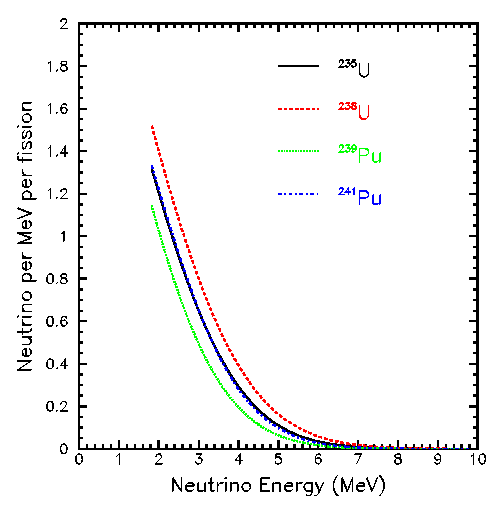
\includegraphics[width=.5\textwidth]{figures/chap2/isotope_antineutrino_spectra.eps}
	\caption{Calculated antineutrinos spectra for each dominant isotope.}
	\label{figure:isotope_antineutrino_spectra}
\end{figure}


\subsection{\texorpdfstring{$\bar{\nu}_e$}{Electron Antineutrino} Detection}
\label{sec:IBD}
Daya Bay utilizes the renowned Cowan–Reines method of prompt-delayed coincidence to detect $\bar{\nu}_e$. The reaction involved in this method is the inverse beta decay (IBD),
\begin{equation}
	\bar{\nu}_e+p\longrightarrow e^++n
\end{equation}
The positron is quickly annihilated by an electron, and photons are released which constitute the prompt signal. The neutron propagates in the target medium, slows down mainly by collisions with protons, and finally gets captured by some nucleus which in turn de-excites and releases photons constituting the delayed signal. Such prompt-delayed coincidence forms a very definitive $\bar{\nu}_e$ signature and greatly suppresses backgrounds.

The antineutrino event rate is given by
\begin{equation}
	R=\int \epsilon(E)P_{\bar{\nu}_e\rightarrow\bar{\nu}_e}(L,E)\frac{N_p\sigma(E)}{4\pi L^2}\phi(E)dE
\end{equation}
where $\epsilon$ is the antineutrino detection efficiency, $P_{\bar{\nu}_e\rightarrow\bar{\nu}_e}$ is the antineutrino survival probability, $N_p$ is the number of free protons in the form of hydrogen in the detector, $\sigma$ is the IBD total cross section, $L$ is the distance from the reactor core to the detector, and $\phi$ is the number of released antineutrinos per unit time given in Eq.~\ref{eq:neutrino_flux}.

$P_{\bar{\nu}_e\rightarrow\bar{\nu}_e}$ depends on $\sin^22\theta_{13}$ which we want to infer from the measured IBD rates. $\epsilon$, $N_p$ and $L$ are measured by auxiliary methods and instruments which will be detailed later. The total cross section of the IBD reaction in the limit of infinite nucleon mass can be written as~\cite{Vogel1999}
\begin{equation}
	\sigma^{(0)}_{tot}=0.0952\times 10^{-42} \left( \frac{E^{(0)}_ep^{(0)}_e}{1 MeV^2}\right) cm^2
\end{equation}
where $E^{(0)}_e$ and $p^{(0)}_e$ are the energy and momentum of the positron, respectively. The next-to-leading order term in $1/M$, the inverse nucleon mass, is nonnegligible. The total cross section to first order in $1/M$ is shown in Figure~\ref{fig:IBD_total_cross_section} and is adopted in Daya Bay's $\theta_{13}$ analysis.
\begin{figure}
	\centering
	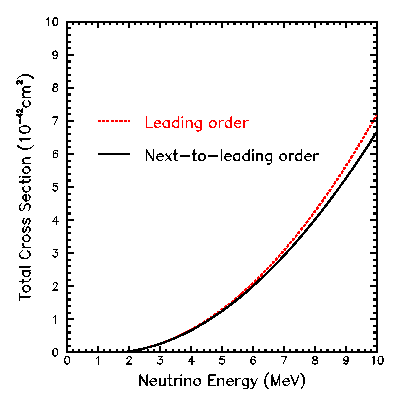
\includegraphics[width=.4\textwidth]{figures/chap2/IBD_total_cross_section.eps}
	\caption{The IBD total cross section calculated to the leading order and next-to-leading order terms.}
	\label{fig:IBD_total_cross_section}
\end{figure}
Combining the average neutrino flux with the IBD total cross section, the expected measured neutrino energy spectrum is shown in Figure~\ref{fig:IBD_rate}.
\begin{figure}
	\centering
	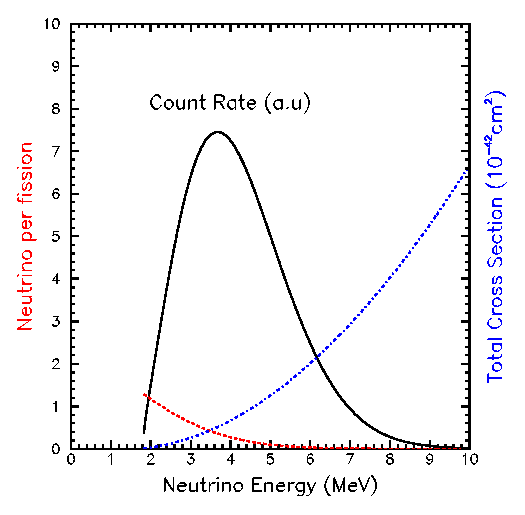
\includegraphics[width=.4\textwidth]{figures/chap2/IBD_rate.eps}
	\caption{The average neutrino flux, the IBD total cross section and the measured neutrino energy spectrum}
	\label{fig:IBD_rate}
\end{figure}


%\subsection{\texorpdfstring{$\theta_{13}$}{Theta13} Analysis and Results}
%The Daya Bay experiment completed 6 antineutrino detector installation in December 2011 and started physics data taking since December 24, 2011. With only barely 2 months of data, Daya Bay showed that $\theta_{13}$ is nonzero with a significance of 5.2 standard deviation and measured $\sin^2{2\theta_{13}}=0.092 \pm 0.016(\text{stat.}) \pm 0.005(\text{syst.})$~\cite{dyb2012_01}. In the following sections details in rate only analysis will be presented as well as the results.
%
%
%\subsubsection{Antineutrino Candidate Selection}
%A Daya Bay antineutrino signal is identified as a pair of prompt-delayed coincidence of triggers. The prompt signal is from the gammas emitted in the electron-positron annihilation process. The energy spectrum of the prompt signal therefore carries the neutrino energy information. Suppose $m_x$, $K_x$, $E_x$ represent the mass, kinetic energy and total energy of particle $x$. From energy conservation of the IBD reaction, we have
%\begin{equation}
%	E_{\bar{\nu}_e}+E_p=E_{e^+}+E_n
%\end{equation}
%The target protons are non-relativistic, $E_p\approx m_p$. Since the positron has a mass much smaller than the neutron, the neutron typically carries only 10-100 keV kinetic energy, which is negligible in the IBD energy scale. The equation becomes
%\begin{equation}
%	E_{\bar{\nu}_e}\approx K_{e^+}+\underbrace{(m_n-m_p)+m_{e^+}}_\text{1.8 MeV}
%\end{equation}
%The equation clearly shows the IBD energy threshold of 1.8 MeV. The measured prompt energy $E_{prompt}$ is the positron kinetic energy plus the annihilation energy $2\times0.511\approx 1.0$ MeV, therefore
%\begin{equation}\label{eq:nu_prompt_relation}
%	E_{\bar{\nu}_e}\approx E_{prompt}+0.8\text{ MeV}
%\end{equation}
%By referring to Figure~\ref{fig:IBD_rate} and Equation~\ref{eq:nu_prompt_relation} and take into account the smearing due to the detector energy resolution, the prompt energy cut is determined to be
%\paragraph{prompt energy cut:}
%\begin{equation}
%	0.7\text{ MeV} < E_{prompt} < 12\text{ MeV}
%\end{equation}
%
%The delayed signal comes from the de-excitation gammas from the neutron capture on $Gd$. Two $Gd$ isotopes contribute to the neutron capture process. $^{155}Gd$ has an energy of 8.536 MeV while $^{157}Gd$ is 7.937 MeV. The delayed energy cut is thus
%\paragraph{delayed energy cut:}
%\begin{equation}
%	6\text{ MeV} < E_{delayed} < 12\text{ MeV}
%\end{equation}
%
%The capture probability of a neutron on Gd between $t$ and $t+dt$ can be written as
%\begin{equation}
%  P_{cap}(E)dt=\sigma(E) n v(E)dt
%\end{equation}
%where $E$ is the neutron energy, $\sigma(E)$ is the total neutron capture cross section, $n$ is the number density of Gd and $v(E)$ is the velocity of the neutron. Figure~\ref{fig:capture_cross_section} shows the capture cross sections for $^{155}$Gd, $^{157}$Gd, $^6$Li, $^1$H, $^{10}$B and $^{113}$Cd~\cite{Bowden2012}.
%\begin{figure}
%  \centering
%  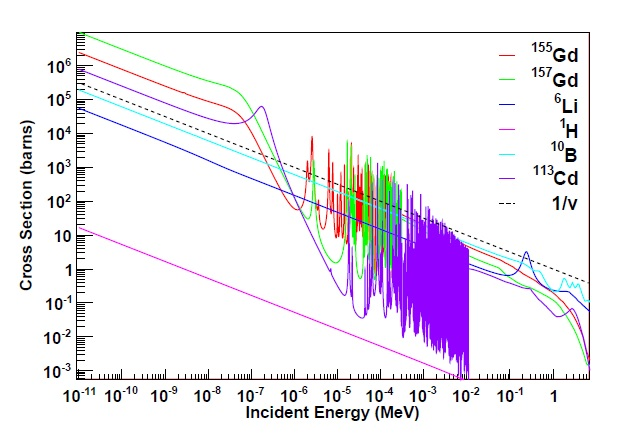
\includegraphics[width=.6\textwidth]{figures/chap2/capture_cross_section.jpg}
%  \caption{Solid lines are the capture cross sections of commonly used capture agents. The dashed line shows the $1/v$ dependence of the capture cross section.}
%  \label{fig:capture_cross_section}
%\end{figure}
%First note that the capture cross section of Gd is 5 orders of magnitude larger than the H. Besides, most elements have a cross section following $1/v$ dependence very well in the entire energy range. If we use the $\sigma(E)\sim 1/v$, $P_{cap}(E)$ is independent of energy and is a constant $\lambda$. If at time $t$, $N(t)$ neutrons survive, then $N(t+dt)=N(t)-P_{cap}dt\cdot N(t)=N(t)-\lambda dtN(t)\Rightarrow N(t)\sim e^{-\lambda t}$. In the case of $^{155}$Gd and $^{157}$Gd, however, when the energy is larger than 0.1 eV, the capture cross sections don't follow a simple $1/v$ dependence and are smaller than a $1/v$ extrapolation from below 0.1 eV. In this case $N(t)\sim e^{-\int P_{cap}dt}$ and the corresponding capture time distribution is
%\begin{equation}
%	-\frac{dN}{dt}\sim P_{cap}(t)e^{-\int P_{cap}(t)dt}
%\end{equation}
%Qualitatively speaking, the capture time distribution is greatly suppressed when $t$ is small since at the moment the neutron has a large energy which implies a small capture probability. The time for a neutron to slow down to thermal energy is called thermalization time. Figure~\ref{fig:capture_time} shows the time between the prompt and the delayed signals in antineutrino candidates.
%\begin{figure}
%	\centering
%	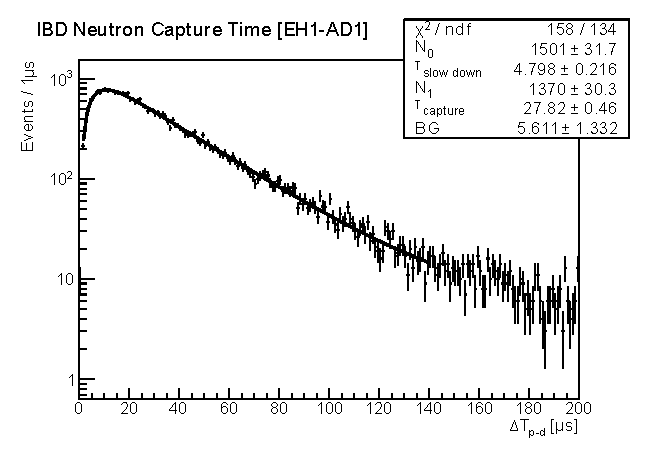
\includegraphics[width=0.6\textwidth]{figures/chap2/capture_time.eps}
%	\caption{Time between the prompt and the delayed events in antineutrino candidates.}
%	\label{fig:capture_time}
%\end{figure}
%The distribution is modeled by
%\begin{equation}
%	C(t)=-C_0e^{-t/t_0}+C_1e^{-t/t_1}+C_{bg}
%\end{equation}
%, where the first term accounts for the the thermalization process, the second term for thermal neutron capture and the third term for background. Here we conclude,
%\paragraph{capture time cut:}
%\begin{equation}
%	1\text{ }\mu\text{s}<\Delta T_{p-d}<200\text{ }\mu\text{s}
%\end{equation}
%
%
%It was found that when photomultiplier tubes are in operation, there could be electronic discharge in the PMT's base. These background events are called flasher events. At Daya Bay, about 5\% of triggers in the antineutrino detector are flasher events. The energy range of the flasher events is from the detector threshold to 100 MeV, and in the delayed signal energy range (6 MeV to 12 MeV) the flasher event rate is 0.7 Hz which is a serious background. Since the flasher events have a different timing and charge patter from physical events, a cut was easily devised to remove such background. The flasher cut is applied to every event before further selection.
%
%If a cosmic muon goes through the AD, many spallation products can be formed. Among them, the spallation neutrons and spallation $^9$Li/$^8$He can lead to prompt-delayed coincidence signal. In order to remove such backgrounds, a muon veto cut is applied which vetos the AD for 1000 $\mu s$ if the muon goes through the AD or 200 $\mu s$ if the muon goes through the water pool but not the AD.
%
%To summarize, the antineutrino candidates must pass:
%\begin{itemize}
%	\item prompt energy cut
%	\item delayed energy cut
%	\item capture time cut
%	\item flasher cut
%	\item muon veto cut
%\end{itemize}
%
%
%\subsubsection{Backgrounds}
%As mentioned in section~\ref{sec:IBD}, the signal of the Daya Bay experiment has a distinct prompt-delayed coincidence in time. However there are still background signals that can mimic such time correlation. The backgrounds of the Daya Bay neutrino experiment are:
%\paragraph{Accidental signals:} Two singles events happening to be in the correlation time window constitute the accidental background. To estimate the accidental rate, first a muon veto cut is applied to remove the non-signal time regions. Then a flasher cut is applied to assure events are physical. To obtain a true singles spectrum, the IBD events now should be removed from it. From the singles spectrum, one can estimate the prompt singles rate $R_p$ (0.7 MeV < E < 12 MeV) and the delayed singles rate $R_d$ (6 MeV < E < 12 MeV). Since the capture time window is (1 $\mu$s, 200 $\mu$s), the accidental background can then be calculated by the rates and the time interval.
%\paragraph{$^9$Li/$^8$He:} Among the various isotopes of the muon spallation products, the long lived $^9$Li/$^8$He can give events faking the IBD signal. Both $^9$Li and $^8$He have a $\beta^-$-n decay channel with a half life of 178.3 ms and 118.5 ms, respectively. To estimate the absolute number of the $^9$Li/$^8$He background, we first look for showering muons (muons deposited a large amount of energy, $>2.5$ GeV). After the showering muons, we look for the prompt-delayed coincidence. Then the timing distribution of the prompt event since the last muon can be used to estimate the number of $^9$Li/$^8$He. In KamLAND, the distribution is then fitted to the function~\cite{KamLAND_01}
%\begin{equation}
%	r(t)=\sum_i \frac{N_i}{\tau_i}e^{-(t-t_\mu)/\tau_i}+r_B
%\end{equation}
%where $i$ runs through those isotopes with similar mean lifetime, $t_\mu$ is the muon time and $N_i$, $\tau_i$ and $r_B$ are the overall number, the mean lifetime and the background, respectively. However for Daya Bay, such a simple formula is not appropriate since Daya Bay is much shallower (1200 m.w.e. at far site) than KanLAND (2700 m.w.e.). With much thicker overburden, the mean time interval between muons is 5 s, which is much larger than the mean lifetime of the isotopes considered. Daya Bay's muon rate can reach 20 Hz, i.e. 50 ms between muons. The isotopes generated by different muons "stacks" before then decay. Therefore a more sophisticated formula too account for the overlapping is required. It is shown that for shallow underground labs, the distribution can be fitted with the function~\cite{Wen2006}
%\begin{equation}
%	ttt
%\end{equation}
%
%
%
%
%
%\section{\texorpdfstring{$\theta_{13}$}{Theta13} Estimation by Rate Analysis}
%Daya Bay set out to do a precise measurement on $\theta_{13}$. More specifically, Daya Bay's physics goal is to reach a sensitivity of $0.01$ in $\sin^22\theta_{13}$ at $90\%$ confidence level. In this section the basic ideas of estimating $\theta_{13}$ from the first 8 weeks of data is presented and more details will be found in the corresponding subsection.
%
%$\theta_{13}$ can be estimated by either the inverse beta decay rate, or by the spectral shape of the neutrino energy spectrum, or in combination. The advantage of the spectral analysis is that it is sensitive to $\Delta m^2$. However since each energy bin can be seen as an independent measurement, it is computationally heavy. Here we will talk about using rate analysis to estimate the value of $\theta_{13}$.
%
%The procedures of estimating $\theta_{13}$ is as follows. First the number of IBD candidate events in a fixed amount of dataset is selected with energy, timing and muon veto cuts. Then the true number of IBD candidates is estimate by correcting for various selection cut efficiency. Besides, all backgrounds that mimic the IBD events are carefully studied and their rates are estimated. The expected number of IBD events is calculated with the knowledge of reactor flux, the IBD total cross section, the detector target mass, the baseline, and the DAQ live time.
%
%\subsection{Expected Number of Inverse Beta Decay Events}
%In the data taking period from Dec. 24 2011 to Feb. 17 2012, Daya Bay has 6 ADs installed and 6 reactor cores in operation. There are 6 measurements from the 6 ADs. Meanwhile the are 6 expected number of IBD events for each AD which are a function of $\sin^22\theta_{13}$. By measuring the number of IBD events and writing the expected number of IBD events as a function of $\theta_{13}$ one can construct a $\chi^2$ function and through minimization $\theta_{13}$ can be estimated.
%
%We will adapt a convention that the subscript $c$ runs through reactor cores and $d$ runs through antineutrino detectors. We want to know the expected number of IBD events for each AD, $T_d$. First we calculate the expected number of IBD events \emph{without} oscillation $N_d$,
%\begin{equation}\label{eq:no_osc_rate}
%	N_d=\sum\limits_{c=1}^6 \epsilon_d N^p_d \int \sigma(E)\frac{\phi_c(E)}{4\pi L_{cd}^2}dE
%\end{equation}
%where $N^p_d$ is the target number density of the $d$th detector, $E$ is the neutrino energy, $\sigma(E)$ is the inverse beta decay total cross section, $\phi_c(E)$ is the neutrino flux from core $c$ and $L_{cd}$ is the baseline from core $c$ to detector $d$. The IBD total cross section is given in \cite{Vogel1999}. The flux from core $c$ is given by Equation~\ref{eq:neutrino_flux} and depends on the instantaneous total thermal power of the reactor core which in general has a core to core difference. The detailed total thermal power is supplied by the nuclear power plant on a daily basis. The baselines are measured by GPS with a precision of 28 mm. The target masses are measure by load cells with a precision of 0.015$\%$. By putting all the information together, the expected IBD events without oscillation can be obtained. Now if we assume the fluxes from all cores have the same energy functional form and only differ in magnitude, $\phi_c=f_c\phi$, then Equation~\ref{eq:no_osc_rate} simplifies to
%\begin{equation}\label{eq:no_osc_rate_simple}
%	N_d=\sum\limits_{c=1}^6 \epsilon_d N^p_d f_c \int \sigma(E)\frac{\phi(E)}{4\pi L_{cd}^2}dE
%\end{equation}
%
%The expected number of IBD events \emph{with} oscillation $T_d$ is
%\begin{equation}\label{eq:with_osc_rate}
%	T_d=\sum\limits_{c=1}^6 \epsilon_d N^p_d f_c \int \sigma(E)P(\theta_{13},L_{cd},E)\frac{\phi(E)}{4\pi L_{cd}^2}dE
%\end{equation}
%The only difference from Equation~\ref{eq:no_osc_rate_simple} is the insertion of the neutrino survival probability, which is given by
%\begin{equation}\label{eq:sur_prob_approx}
%	P(\theta_{13},L_{cd},E)=1-\sin^22\theta_{13}\sin^2(1.267\Delta m_{32}^2L_{cd}/E)
%\end{equation}
%Here we have used $\Delta m_{31}^2=2.32^{+0.12}_{-0.08}\times 10^{-3} eV^2\approx \Delta m_{32}^2$ and kept only the leading term at Daya Bay's baseline. Substituting Equation~\ref{eq:sur_prob_approx} back to Equation~\ref{eq:with_osc_rate}, we have
%\begin{equation}\label{eq:with_osc_rate_2}
%	T_d=N_d-\sin^22\theta_{13}\frac{N^p_d}{4\pi}\sum\limits_{c}\frac{f_c}{L_{cd}^2}\int\sigma\sin^2\left(\frac{1.267\Delta m_{32}^2L_{cd}}{E}\right)\phi dE
%\end{equation}
%If we define weight by
%\begin{equation}\label{eq:omega}
%	\omega_{cd}=\frac{f_c/L_{cd}^2}{\sum\limits_{c} f_c/L_{cd}^2}
%\end{equation}
%and oscillation factor by
%\begin{equation}\label{eq:Delta}
%	\Delta_{cd}=\frac{\int\sigma\sin^2\left(\frac{1.267\Delta m_{32}^2L_{cd}}{E}\right)\phi dE}{\int\sigma\phi dE}
%\end{equation}
%and divide Equation~\ref{eq:with_osc_rate_2} by $N_d$, we arrive at the result
%\begin{equation}\label{eq:with_osc_rate_final}
%	\frac{T_d}{N_d}=1-\sin^22\theta_{13}\sum\limits_{c}\omega_{cd}\Delta_{cd}
%\end{equation}
%$N_d$ was calculated previously, and $\omega_{cd}$ and $\Delta_{cd}$ can also be calculated from available data, so $T_d$ can be expressed as a function of the one parameter to be estimated, namely $\sin^22\theta_{13}$. If we call the second term in Equation~\ref{eq:with_osc_rate_final} oscillation deficit, the result in this data taking period is shown in Table~\ref{table:ocs_deficit}.
%\begin{table}
%  \centering
%	\begin{tabular}{|c|c|c|c|c|c|}
%		\hline
%		AD1 & AD2 & AD3 & AD4 & AD5 & AD6 \\
%		\hline
%		0.148$\sin^22\theta_{13}$ & 0.145$\sin^22\theta_{13}$ & 0.20$\sin^22\theta_{13}$ & 0.77$\sin^22\theta_{13}$ & 0.77$\sin^22\theta_{13}$ & 0.77$\sin^22\theta_{13}$ \\
%		\hline
%	\end{tabular}
%	\caption{Oscillation deficit for six ADs}
%	\label{table:ocs_deficit}
%\end{table}
%
%
%\begin{table}
%	\centering
%	\begin{tabular}{|c|c|c|c|c|c|c|}
%		\hline
%		detector & AD1 & AD2 & AD3 & AD4 & AD5 & AD6 \\
%		\hline
%		\hline
%		IBD candidates & 28935 & 28975 & 22466 & 3528 & 3436 & 3452 \\
%		\hline
%		total backgrounds & 556.19 & 441 & 358 & 145 & 148 & 139 \\
%		\hline
%	\end{tabular}
%	\caption{IBD analysis results}
%	\label{table:IBD}
%\end{table}
%
%\begin{table}
%	\centering
%	\begin{tabular}{|c|c|c|c|c|c|c|}
%	\hline
%	detector & AD1 & AD2 & AD3 & AD4 & AD5 & AD6 \\
%	\hline
%	\hline
%	measured IBD number & 28379 & 28418 & 22034 & 3354.3 & 3260.4 & 3286.1 \\
%	\hline
%	predicted IBD number & 28083 & 28522 & 21895 & 3496.3 & 3502.6 & 3466.3 \\
%	\hline
%	measured/predicted & 101.0$\%$ & 99.6$\%$ & 100.6$\%$ & 95.9$\%$ & 93.9$\%$ & 94.8$\%$ \\
%	\hline
%	\end{tabular}
%	\caption{ratio of number of measured and predicted IBD events.}
%	\label{table:IBD_ratio}
%\end{table}
%
%Table~\ref{table:IBD} shows the analysis results of number of IBD candidates and total backgrounds. Table~\ref{table:IBD_ratio} shows the number of measured IBD events with background subtracted, the number of predicted IBD events \emph{without} oscillation, and the ratio of the two numbers. A heuristic way to estimate $\sin^22\theta_{13}$ is to take the ratios from any 2 ADs, form the difference, and compare with the same difference with numbers taken from Table~\ref{table:ocs_deficit}. For example if we take AD1 and AD6, we have $(0.77-0.148)\sin^22\theta_{13}=101\%-94.8\%$, or $\sin^22\theta_{13}=0.099$.
%
%Another way to estimate $\sin^22\theta_{13}$ is to use the so called "relative measurement", i.e. by forming the ratio of two IBD rates registered by two different detectors. By this way we don't have to rely on the absolute calculation of $N_d$ and the systematic uncertainties concerning to the absolute reactor flux will cancel when forming the ratio. To start with, we take one of the far site AD and denote quantities concerning to the AD by subscript $d=F$. Meanwhile we take a near site AD and denote quantities with subscript $d=N$. The ratio of the two estimated rates is
%\begin{equation}\label{eq:relative1}
%	\frac{T_F}{T_N}=\frac{\epsilon_F}{\epsilon_N}\frac{\sum\limits_c \frac{N^p_df_c}{4\pi L^2_{cF}}\int\sigma\phi P_{cF}dE}{\sum\limits_c \frac{N^p_df_c}{4\pi L^2_{cN}}\int\sigma\phi P_{cN}dE}
%\end{equation}
%If we further assume that the target mass $N^p_d$ is the same across detectors, Equation~\ref{eq:relative1} simplfies to
%\begin{equation}
%	\frac{T_F}{T_N}=\frac{\epsilon_F}{\epsilon_N}\frac{\sum\limits_c \frac{f_c}{L^2_{cF}}\int\sigma\phi P_{cF}dE}{\sum\limits_c \frac{f_c}{L^2_{cN}}\int\sigma\phi P_{cN}dE}
%\end{equation}
%Now by employing Equation~\ref{eq:sur_prob_approx},~\ref{eq:omega} and~\ref{eq:Delta}, we have
%\begin{eqnarray}
%	\frac{T_F}{T_N}&=&\frac{\epsilon_F}{\epsilon_N}\frac{\frac{1}{\bar{L}^2_F}\sum\limits_c \omega_{cF}\left( 1-\sin^22\theta_{13}\Delta_{cF} \right)}{\frac{1}{\bar{L}^2_N}\sum\limits_c \omega_{cN}\left( 1-\sin^22\theta_{13}\Delta_{cN} \right)} \\
%	&=&\frac{\epsilon_F}{\epsilon_N}\frac{\bar{L}^2_N}{\bar{L}^2_F}\frac{1-\sin^22\theta_{13}\sum\limits_c\omega_{cF}\Delta_{cF}}{1-\sin^22\theta_{13}\sum\limits_c\omega_{cN}\Delta_{cN}}
%\end{eqnarray}
%where we have defined the flux-weighted baseline $\bar{L}_d$ as
%\begin{equation}
%	\frac{1}{\bar{L}^2_d}=\sum\limits_c \frac{f_c}{L_{cd}^2}
%\end{equation}
%and used the identity $\sum\limits_c\omega_{cd}=1$ for all $d$.
%The unblinded baselines $L_{cd}$ from core $c$ to detector $d$ is tabulated in Table~\ref{table:baseline}.
%\begin{table}
%	\centering
%	\begin{tabular}{|c|c|c|c|c|c|c|}
%		\hline
%		(m) & D1 & D2 & L1 & L2 & L3 & L4 \\
%		\hline
%		AD1 & 362.3773 & 371.759 & 903.4704 & 817.1618 & 1353.622 & 1265.319 \\
%		AD2 & 357.9373 & 368.4106 & 903.3506 & 816.9001 & 1354.233 & 1265.89 \\
%		AD3 & 1332.475 & 1358.144 & 467.5708 & 489.5737 & 557.5798 & 499.2072 \\
%		AD4 & 1919.63 & 1894.335 & 1533.177 & 1533.625 & 1551.381 & 1524.937 \\
%		AD5 & 1917.516 & 1891.974 & 1534.916 & 1535.029 & 1554.764 & 1528.043 \\
%		AD6 & 1925.253 & 1899.859 & 1538.927 & 1539.465 & 1556.341 & 1530.076 \\
%		\hline
%	\end{tabular}
%	\caption{Baselines between reactor cores and ADs. D means Daya Bay power plant and L means Ling Ao power plant.}
%	\label{table:baseline}
%\end{table}
%The reactor thermal power for each reactor core is provided by the nuclear power plant in the form of daily average and is stored and readily accessed in Daya Bay's offline database. Therefore $\bar{L}_d$, $\omega_{cd}$ and $\Delta_{cd}$ can be calculated and are listed in Table~\ref{table:weighted_baseline}, Table~\ref{table:weight} and Table~\ref{table:osc_factor}.
%\begin{table}
%	\centering
%	\begin{tabular}{|c|c|c|c|c|c|c|}
%		\hline
%		detector & AD1 & AD2 & AD3 & AD4 & AD5 & AD6 \\
%		\hline
%		flux-weighted baseline (m) & 497 & 491 & 554 & 1627 & 1628 & 1632 \\
%		\hline
%	\end{tabular}
%	\caption{Flux-weighted baselines for 6 ADs.}
%	\label{table:weighted_baseline}
%\end{table}
%\begin{table}
%	\centering
%	\begin{tabular}{|c|c|c|c|c|c|c|}
%		\hline
%		 & D1 & D2 & L1 & L2 & L3 & L4 \\
%		\hline
%		AD1 & 0.417562 &0.426367 &0.0383572 &0.0539022 &0.0300287 &0.0337836 \\
%		AD2 & 0.420337 &0.426393 &0.0376817 &0.0529728 &0.0294655 &0.0331499 \\
%		AD3 & 0.0411601 &0.0425759 &0.190634 &0.20044 &0.235894 &0.289297 \\
%		AD4 & 0.140358 &0.154889 &0.125564 &0.143849 &0.215749 &0.219591 \\
%		AD5 & 0.140904 &0.155538 &0.12549 &0.143828 &0.215173 &0.219068 \\
%		AD6 & 0.140465 &0.155011 &0.125454 &0.143706 &0.215798 &0.219566 \\
%		\hline
%	\end{tabular}
%	\caption{Weight table}
%	\label{table:weight}
%\end{table}
%\begin{table}
%	\centering
%	\begin{tabular}{|c|c|c|c|c|c|c|}
%		\hline
%		 & D1 & D2 & L1 & L2 & L3 & L4 \\
%		\hline
%		AD1 & 0.0826245 &0.0855193 &0.415679 &0.352319 &0.683062 &0.639695 \\
%		AD2 & 0.0806925 &0.0840498 &0.415596 &0.35214 &0.683346 & 0.639996 \\
%		AD3 & 0.676348 &0.682713 &0.133883 &0.144174 &0.183527 &0.150169 \\
%		AD4 & 0.812616 &0.811365 &0.756031 &0.752377 &0.758721 &0.750827 \\
%		AD5 & 0.812625 &0.811305 &0.75657 &0.75282 &0.759727 &0.751819 \\
%		AD6 & 0.812577 &0.811492 &0.757804 &0.754208 &0.760193 &0.752464 \\
%		\hline
%	\end{tabular}
%	\caption{Oscillation factor}
%	\label{table:osc_factor}
%\end{table}
%\begin{table}
%	\scriptsize
%	\centering
%	\begin{tabular}{|c|c|c|c|c|c|c|}
%		\hline
%		 & AD1 & AD2 & AD3 & AD4 & AD5 & AD6 \\
%		\hline
%		IBD candidates & 28935 & 28975 & 22466 & 3528 & 3436 & 3452 \\
%		veto cut efficiency & 0.8019 & 0.7989 & 0.8363 & 0.9547 & 0.9543 & 0.9538 \\
%		Accidentals (per day) & 9.82±0.06 & 9.88±0.06 & 7.67±0.05 & 3.29±0.03 & 3.33±0.03 & 3.12±0.03 \\
%		Fast-neutron (per day) & 0.84±0.28 & 0.84±0.28 & 0.74±0.44 & 0.04±0.04 & 0.04±0.04 & 0.04±0.04 \\
%		$^9$Li/$^8$He (per AD per day) & 3.1±1.6 & 3.1±1.6 & 1.8±1.1 & 1.8±1.1 & 0.16±0.11 & 0.16±0.11 \\
%		Am-C correlated (per AD per day) & 0.2±0.2 & 0.2±0.2 & 0.2±0.2 & 0.2±0.2 & 0.2±0.2 & 0.2±0.2 \\
%		$^{13}$C($\alpha$,n)$^{16}$O background (per day) & 0.04±0.02 & 0.04±0.02 & 0.035±0.02 & 0.03±0.02 & 0.03±0.02 & 0.03±0.02 \\
%		\hline
%	\end{tabular}
%	\caption{Signal and background summary}
%	\label{table:bkg_sig}
%\end{table}





\section{\texorpdfstring{$\theta_{13}$}{Theta13} Estimation by Rate Analysis}
Daya Bay set out to do a precise measurement on $\theta_{13}$. More specifically, Daya Bay's physics goal is to reach a sensitivity of $0.01$ in $\sin^22\theta_{13}$ at $90\%$ confidence level. In this section the basic ideas of estimating $\theta_{13}$ from the first 8 weeks of data is presented and more details will be found in the corresponding subsection.

$\theta_{13}$ can be estimated by either the inverse beta decay rate, or by the spectral shape of the neutrino energy spectrum, or in combination. The advantage of the spectral analysis is that it is sensitive to $\Delta m^2$. However, since each energy bin can be seen as an independent measurement, the analysis is much more involved. Here we will talk about using rate only analysis to estimate the value of $\theta_{13}$.

The procedures of estimating $\theta_{13}$ is as follows. First the IBD candidate events in a certain fixed amount of dataset is selected with energy, timing and muon veto cuts. Then the true number of IBD candidates is estimate by correcting for various selection cut efficiency. Besides, all backgrounds that mimic the IBD events are carefully studied and their rates are estimated. The expected number of IBD events is calculated with the knowledge of reactor flux, the IBD total cross section, the detector target mass, the baseline, and the DAQ live time.

\subsection{Expected and Measured Number of Inverse Beta Decay Events}
The Daya Bay experiment started data taking on 24 December 2011 with 6 antineutrino detectors (ADs). Data taking was paused on 28 July 2012 and two new ADs were installed. Operation of the full experiment with all 8 ADs started on 19 October 2012. In this discussion we use 404 days of data acquired in the 8-AD period combined with all 217 days of data acquired in the 6-AD period. Each AD has one measurement of number of IBD events. Meanwhile for each AD, one expected, i.e., no oscillation, the number of IBD events which is a function of $\sin^22\theta_{13}$ can be calculated. By measuring the number of IBD events and writing the expected number of IBD events as a function of $\theta_{13}$, one can construct a $\chi^2$ function, and through minimization $\theta_{13}$ can be estimated.

We will adopt a convention that the subscript $c$ runs through reactor cores and $d$ runs through antineutrino detectors. We want to know the expected number of IBD events for each AD, $T_d$. First we calculate the expected number of IBD events \emph{without} oscillation $N_d$,
\begin{equation}\label{eq:no_osc_rate}
	N_d=\sum\limits_{c=1}^6 \epsilon_d N^p_d \int \sigma(E)\frac{\phi_c(E)}{4\pi L_{cd}^2}dE
\end{equation}
where $N^p_d$ is the target number density of the $d$th detector, $E$ is the neutrino energy, $\sigma(E)$ is the inverse beta decay total cross section, $\phi_c(E)$ is the neutrino flux from core $c$, and $L_{cd}$ is the baseline from core $c$ to detector $d$. The IBD total cross section is given in \cite{Vogel1999}. The flux from core $c$ is given by Equation~\ref{eq:neutrino_flux} and depends on the instantaneous total thermal power of the reactor core which in general has a core to core difference. The detailed total thermal power is supplied by the nuclear power plant on a daily basis~\cite{docdb7610}. The baselines are measured by GPS with a precision of 28 mm~\cite{dayabay2013}. The target masses are measure by load cells with a precision of 0.015$\%$. By putting all the information together, the expected IBD events without oscillation can be obtained. Now if we assume the fluxes from all cores have the same energy functional form and only differ in magnitude, $\phi_c=f_c\phi$, then Equation~\ref{eq:no_osc_rate} simplifies to
\begin{equation}\label{eq:no_osc_rate_simple}
	N_d=\sum\limits_{c=1}^6 \epsilon_d N^p_d f_c \int \sigma(E)\frac{\phi(E)}{4\pi L_{cd}^2}dE
\end{equation}

The expected number of IBD events \emph{with} oscillation $T_d$ is
\begin{equation}\label{eq:with_osc_rate}
	T_d=\sum\limits_{c=1}^6 \epsilon_d N^p_d f_c \int \sigma(E)P(\theta_{13},L_{cd},E)\frac{\phi(E)}{4\pi L_{cd}^2}dE
\end{equation}
The only difference from Equation~\ref{eq:no_osc_rate_simple} is the insertion of the neutrino survival probability, which is given by
\begin{equation}\label{eq:sur_prob_approx}
	P(\theta_{13},L_{cd},E)=1-\sin^22\theta_{13}\sin^2(1.267\Delta m_{32}^2L_{cd}/E)
\end{equation}
Here we have used $\Delta m_{31}^2=2.32^{+0.12}_{-0.08}\times 10^{-3} eV^2\approx \Delta m_{32}^2$ and kept only the leading term at Daya Bay's baseline. Substituting Equation~\ref{eq:sur_prob_approx} back to Equation~\ref{eq:with_osc_rate}, we have
\begin{equation}\label{eq:with_osc_rate_2}
	T_d=N_d-\sin^22\theta_{13}\frac{N^p_d}{4\pi}\sum\limits_{c}\frac{f_c}{L_{cd}^2}\int\sigma\sin^2\left(\frac{1.267\Delta m_{32}^2L_{cd}}{E}\right)\phi dE
\end{equation}
If we define weight by
\begin{equation}\label{eq:omega}
	\omega_{cd}=\frac{f_c/L_{cd}^2}{\sum\limits_{c} f_c/L_{cd}^2}
\end{equation}
and oscillation factor by
\begin{equation}\label{eq:Delta}
	\Delta_{cd}=\frac{\int\sigma\sin^2\left(\frac{1.267\Delta m_{32}^2L_{cd}}{E}\right)\phi dE}{\int\sigma\phi dE}
\end{equation}
and divide Equation~\ref{eq:with_osc_rate_2} by $N_d$, we arrive at the result
\begin{equation}\label{eq:with_osc_rate_final}
	\frac{T_d}{N_d}=1-\sin^22\theta_{13}\sum\limits_{c}\omega_{cd}\Delta_{cd}
\end{equation}
$N_d$ was calculated previously, and $\omega_{cd}$ and $\Delta_{cd}$ can also be calculated from available data, so $T_d$ can be expressed as a function of the one parameter to be estimated, namely $\sin^22\theta_{13}$. If we call the second term in Equation~\ref{eq:with_osc_rate_final} oscillation deficit, the result in these data taking period is shown in Table~\ref{table:ocs_deficit}.
\begin{table}
  \centering
	\begin{tabular}{|c|c|c|c|c|c|}
		\hline
		AD1 & AD2 & AD3 & AD4 & AD5 & AD6 \\
		\hline
		0.148$\sin^22\theta_{13}$ & 0.145$\sin^22\theta_{13}$ & 0.20$\sin^22\theta_{13}$ & 0.77$\sin^22\theta_{13}$ & 0.77$\sin^22\theta_{13}$ & 0.77$\sin^22\theta_{13}$ \\
		\hline
	\end{tabular}
	\caption{Oscillation deficit for six ADs}
	\label{table:ocs_deficit}
\end{table}


\begin{table}
	\centering
	\begin{tabular}{|c|c|c|c|c|c|c|}
		\hline
		detector & AD1 & AD2 & AD3 & AD4 & AD5 & AD6 \\
		\hline
		\hline
		IBD candidates & 28935 & 28975 & 22466 & 3528 & 3436 & 3452 \\
		\hline
		total backgrounds & 556.19 & 441 & 358 & 145 & 148 & 139 \\
		\hline
	\end{tabular}
	\caption{IBD analysis results}
	\label{table:IBD}
\end{table}

\begin{table}
	\centering
	\begin{tabular}{|c|c|c|c|c|c|c|}
	\hline
	detector & AD1 & AD2 & AD3 & AD4 & AD5 & AD6 \\
	\hline
	\hline
	measured IBD number & 28379 & 28418 & 22034 & 3354.3 & 3260.4 & 3286.1 \\
	\hline
	predicted IBD number & 28083 & 28522 & 21895 & 3496.3 & 3502.6 & 3466.3 \\
	\hline
	measured/predicted & 101.0$\%$ & 99.6$\%$ & 100.6$\%$ & 95.9$\%$ & 93.9$\%$ & 94.8$\%$ \\
	\hline
	\end{tabular}
	\caption{ratio of number of measured and predicted IBD events.}
	\label{table:IBD_ratio}
\end{table}

Table~\ref{table:IBD} shows the analysis results of number of IBD candidates and total backgrounds. Table~\ref{table:IBD_ratio} shows the number of measured IBD events with background subtracted, the number of predicted IBD events \emph{without} oscillation, and the ratio of the two numbers. A heuristic way to estimate $\sin^22\theta_{13}$ is to take the ratios from any 2 ADs, form the difference, and compare with the same difference with numbers taken from Table~\ref{table:ocs_deficit}. For example if we take AD1 and AD6, we have $(0.77-0.148)\sin^22\theta_{13}=101\%-94.8\%$, or $\sin^22\theta_{13}=0.099$.

Another way to estimate $\sin^22\theta_{13}$ is to use the so called ``relative measurement"~\cite{Mikaelyan2000}, i.e. by forming the ratio of two IBD rates registered by two different detectors. By this way we don't have to rely on the absolute calculation of $N_d$ and the systematic uncertainties concerning to the absolute reactor flux will cancel when forming the ratio. To start with, we take one of the far site AD and denote quantities concerning to the AD by subscript $d=F$. Meanwhile we take a near site AD and denote quantities with subscript $d=N$. The ratio of the two estimated rates is
\begin{equation}\label{eq:relative1}
	\frac{T_F}{T_N}=\frac{\epsilon_F}{\epsilon_N}\frac{\sum\limits_c \frac{N^p_df_c}{4\pi L^2_{cF}}\int\sigma\phi P_{cF}dE}{\sum\limits_c \frac{N^p_df_c}{4\pi L^2_{cN}}\int\sigma\phi P_{cN}dE}
\end{equation}
If we further assume that the target mass $N^p_d$ and the reactor flux $f_c\phi$ are the same across detectors, Equation~\ref{eq:relative1} simplfies to
\begin{equation}
	\frac{T_F}{T_N}=\frac{\epsilon_F}{\epsilon_N}\frac{\sum\limits_c \frac{1}{L^2_{cF}}\int\sigma\phi P_{cF}dE}{\sum\limits_c \frac{1}{L^2_{cN}}\int\sigma\phi P_{cN}dE}
\end{equation}
Now by employing Equation~\ref{eq:sur_prob_approx},~\ref{eq:omega} and~\ref{eq:Delta} and set $f_c=1$, we have
\begin{eqnarray}
	\frac{T_F}{T_N}&=&\frac{\epsilon_F}{\epsilon_N}\frac{\frac{1}{\bar{L}^2_F}\sum\limits_c \omega_{cF}\left( 1-\sin^22\theta_{13}\Delta_{cF} \right)}{\frac{1}{\bar{L}^2_N}\sum\limits_c \omega_{cN}\left( 1-\sin^22\theta_{13}\Delta_{cN} \right)} \\
	&=&\frac{\epsilon_F}{\epsilon_N}\frac{\bar{L}^2_N}{\bar{L}^2_F}\frac{1-\sin^22\theta_{13}\sum\limits_c\omega_{cF}\Delta_{cF}}{1-\sin^22\theta_{13}\sum\limits_c\omega_{cN}\Delta_{cN}}
\end{eqnarray}
where we have defined the flux-weighted baseline $\bar{L}_d$ as
\begin{equation}
	\frac{1}{\bar{L}^2_d}=\sum\limits_c \frac{1}{L_{cd}^2}
\end{equation}
and used the identity $\sum\limits_c\omega_{cd}=1$ for all $d$.
The unblinded baselines $L_{cd}$ from core $c$ to detector $d$ is tabulated in Table~\ref{table:baseline}.
\begin{table}
	\centering
	\begin{tabular}{|c|c|c|c|c|c|c|}
		\hline
		(m) & D1 & D2 & L1 & L2 & L3 & L4 \\
		\hline
		AD1 & 362.3773 & 371.759 & 903.4704 & 817.1618 & 1353.622 & 1265.319 \\
		AD2 & 357.9373 & 368.4106 & 903.3506 & 816.9001 & 1354.233 & 1265.89 \\
		AD3 & 1332.475 & 1358.144 & 467.5708 & 489.5737 & 557.5798 & 499.2072 \\
		AD4 & 1919.63 & 1894.335 & 1533.177 & 1533.625 & 1551.381 & 1524.937 \\
		AD5 & 1917.516 & 1891.974 & 1534.916 & 1535.029 & 1554.764 & 1528.043 \\
		AD6 & 1925.253 & 1899.859 & 1538.927 & 1539.465 & 1556.341 & 1530.076 \\
		\hline
	\end{tabular}
	\caption{Baselines between reactor cores and ADs. D means Daya Bay power plant and L means Ling Ao power plant.}
	\label{table:baseline}
\end{table}
If we let $\sum\limits_c\omega_{cd}\Delta_{cd}=\Omega_d$ and $\frac{T_F}{T_N}\frac{\epsilon_N}{\epsilon_F}\frac{\bar{L}^2_F}{\bar{L}^2_N}=\Delta$ and rearrange, we have
\begin{equation}\label{eq:theta13_relative}
	\sin^22\theta_{13}=\frac{1-\Delta}{\Omega_F-\Delta\Omega_N}
\end{equation}
The most recent results of eight antineutrino detectors are summarized in Table~\ref{table:IBD_summary}
\begin{table}
	\centering
	\begin{tabular}{c|cc|cc}
		\hline
		\hline
    & AD1 & AD2 & AD3 & AD8 \\
    \hline
		IBD candidates & 202461 & 206217 & 193356 & 190046 \\
		DAQ live time(day) & \multicolumn{2}{c|}{374.447} & \multicolumn{2}{c}{378.407} \\
		$\epsilon_\mu$ & 0.8255 & 0.8223 & 0.8574 & 0.8577 \\
		$\epsilon_m$ & 0.9746 & 0.9749 & 0.9759 & 0.9756 \\
		Accidentals(/day) & 8.62$\pm$0.09 & 8.76$\pm$0.09 & 6.43$\pm$0.07 & 6.86$\pm$0.07 \\
		Fast neutron(/day) & \multicolumn{2}{c|}{0.78$\pm$0.12} & \multicolumn{2}{c}{0.54$\pm$0.19} \\
		$^9$Li/$^8$He(/day) & \multicolumn{2}{c|}{2.8$\pm$1.5} & \multicolumn{2}{c}{1.7$\pm$0.9} \\
		AmC correlated(/day) & 0.20$\pm$0.09 & 0.21$\pm$0.10 & 0.18$\pm$0.08 & 0.22$\pm$0.10 \\
		$^{13}$C($\alpha$,n)$^{16}$O(/day) & 0.08$\pm$0.04 & 0.07$\pm$0.04 & 0.05$\pm$0.03 & 0.07$\pm$0.04 \\
		\hline
		IBD rate(/day) & 659.58$\pm$2.12 & 674.36$\pm$2.14 & 601.77$\pm$1.67 & 590.87$\pm$1.66 \\
		\hline
		side-by-side IBD rate ratio & \multicolumn{2}{c|}{0.978$\pm$0.004} & \multicolumn{2}{c}{1.019$\pm$0.004} \\
		\hline
		\hline
	\end{tabular}\\
	\begin{tabular}{c|cccc}
		\hline
		\hline
		& AD4 & AD5 & AD6 & AD7 \\
    \hline
		IBD candidates & 27067 & 27389 & 27032 & 27419 \\
		DAQ live time(day) & \multicolumn{4}{c}{372.685} \\
		$\epsilon_\mu$ & 0.9811 & 0.9811 & 0.9808 & 0.9811 \\
		$\epsilon_m$ & 0.9762 & 0.976 & 0.9757 & 0.9758 \\
		Accidentals(/day) & 1.07$\pm$0.01 & 0.94$\pm$0.01 & 0.94$\pm$0.01 & 1.26$\pm$0.01 \\
		Fast neutron(/day) & \multicolumn{4}{c}{0.05$\pm$0.01} \\
		$^9$Li/$^8$He(/day) & \multicolumn{4}{c}{0.27$\pm$0.14} \\
		AmC correlated(/day) & 0.06$\pm$0.03 & 0.04$\pm$0.02 & 0.04$\pm$0.02 & 0.07$\pm$0.02 \\
		$^{13}$C($\alpha$,n)$^{16}$O(/day) & 0.05$\pm$0.03 & 0.05$\pm$0.03 & 0.05$\pm$0.03 & 0.05$\pm$0.03 \\
		\hline
		IBD rate(/day) & 74.33$\pm$0.48 & 75.40$\pm$0.49 & 74.44$\pm$0.48 & 75.15$\pm$0.49 \\
		\hline
		side-by-side IBD rate ratio & \multicolumn{4}{c}{} \\
		\hline
		\hline
	\end{tabular}
	\caption{Signal and background summary for eight AD period. Note that the backgrounds are efficiency corrected.}
	\label{table:IBD_summary}
\end{table}
If we take $F=AD4$ and $N=AD3$, we have
\begin{equation}
	\frac{\bar{L}^2_F}{\bar{L}^2_N}=\frac{170.81}{22.462}
\end{equation}
Now we want to estimate $\Delta$.
\begin{equation}
	\Delta=\left( \frac{T_F}{\epsilon_F} \right) \Big/ \left( \frac{T_N}{\epsilon_N} \right)\cdot \left(\frac{\bar{L}^2_F}{\bar{L}^2_N} \right)
\end{equation}
Since the ratio of the number of IBD events is the same as the ratio of the IBD rates, $\Delta$ can also be written as
\begin{equation}
	\Delta=\left(\frac{R_{IBD,F}}{R_{IBD,N}}\right) \cdot \left(\frac{\bar{L}^2_F}{\bar{L}^2_N} \right)
\end{equation}
Here $R_{IBD,d}$ is the true IBD rate for detector $d$ \emph{after} efficiency correction. To obtain $R_{IBD,d}$ from Table~\ref{table:IBD_summary}, note that the background numbers are efficiency corrected. Therefore for a detector $d$,
\begin{equation}
	R_{IBD}=\frac{N_{IBDc}}{\epsilon_\mu\epsilon_m T_{life}}-R_{acc}-R_{fn}-R_{iso}-R_{AmC}-R_{^{13}C}
\end{equation}
where $N_{IBDc}$ is the number of IBD candidates, $\epsilon_\mu$ is the muon veto cut efficiency, $\epsilon_m$ is the multiplicity cut efficiency, $T_{life}$ is the DAQ life time, $R_{acc}$ is the accidentals rate, $R_{fn}$ is the fast neutron rate, $R_{iso}$ is the $^9$Li/$^8$He rate, $R_{AmC}$ is the AmC correlated background rate, and $R_{^{13}C}$ is the $^{13}$C($\alpha$,n)$^{16}$O rate. This is how the numbers in the row ``IBD rate(/day)'' are obtained. Take the IBD rate numbers from AD3 for near detector and AD4 for far detector, we can obtain $\Delta$,
\begin{equation}\label{eq:Delta_value}
	\Delta=\left(\frac{74.33}{601.77}\right)\left(\frac{170.81}{22.462}\right)=0.939
\end{equation}
It is known that
\begin{equation}\label{eq:Omega_value}
	\Omega_{AD4}-\Delta\Omega_{AD3}\approx \Omega_{AD4}-\Omega_{AD3}\approx 0.6
\end{equation}
By Equations~\ref{eq:theta13_relative},~\ref{eq:Delta_value} and~\ref{eq:Omega_value}, we have
\begin{equation}
	\boxed{\sin^22\theta_{13}=0.102}
\end{equation}
%The IBD rate is estimated by the following formula,
%\begin{equation}
%	R_{IBD}=\frac{N_{IBDc}}{\epsilon_\mu\epsilon_m T_{life}}-R_{acc}-R_{fn}-R_{iso}-R_{AmC}-R_{^{13}C}
%\end{equation}
% If we suppose the backgrounds are uncorrelated, the error in the IBD rate can be obtained by quadrature,
%\begin{equation}
%	\delta R_{IBD}=\sqrt{\left(\frac{\sqrt{N_{IBDc}}}{\epsilon_\mu\epsilon_m T_{life}}\right)^2+\delta R_{acc}^2+\delta R_{fn}^2+\delta R_{iso}^2+\delta R_{AmC}^2+\delta R_{^{13}C}^2}
%\end{equation}


\section{Uncertainty Analysis}
Now we want to estimate the error in $\sin^22\theta_{13}$. Start with Equation~\ref{eq:theta13_relative}, the leading term in the uncertainty in $\sin^22\theta_{13}$ is
\begin{equation}
	\delta(\sin^22\theta_{13})\approx\frac{\delta\Delta}{\Omega_F-\Delta\Omega_N}
\end{equation}
Write out $\delta\Delta$ with the error propagation formula and assume it is dominated by the uncertainty due to the far site detector and therefore the near site and the correlation between near and far sites can all be neglected, we have
\begin{equation}
	\frac{\delta\Delta}{\Delta}=\frac{\delta R_{IBD,F}}{R_{IBD,F}}
\end{equation}
From now on the subscript ``$F$'' is omitted and we know the rates involved refer to the far detector rates. Since statistic uncertainties improve over time, if we want to know the final sensitivity of the experiment, we can decompose the total uncertainty into the contributions from systematic and statistical uncertainties. The statistical uncertainty in $\delta R_{IBD}$ is
\begin{equation}
	\frac{\delta R_{IBD}^{stat}}{R_{IBD}}\approx\frac{\delta N_{IBDc}}{N_{IBDc}}=\frac{1}{\sqrt{N_{IBDc}}}
\end{equation}
If we utilize IBD data from all four far site ADs, we have
\begin{equation}
	\frac{\delta R_{IBD}^{stat}}{R_{IBD}}\approx\frac{1}{\sqrt{27000\times 4}}\approx 0.003
\end{equation}
Thus
\begin{equation}
	\delta(\sin^22\theta_{13})^{stat}=\frac{\delta\Delta^{stat}}{\Omega_F-\Delta\Omega_N}=\frac{\Delta\left(\frac{\delta R_{IBD}^{stat}}{R_{IBD}}\right)}{\Omega_F-\Delta\Omega_N}=\frac{0.939\times 0.003}{0.6}=0.005
\end{equation}

The systematic uncertainty right now is dominated by $^9$Li/$^8$He background. When summed in quadrature, this term dominates,
\begin{equation}
	\frac{R_{IBD}^{syst}}{R_{IBD}}\approx\frac{\delta R_{iso}}{R_{IBD}}\approx \frac{0.14}{74}\approx 0.002
\end{equation}
Thus
\begin{equation}
	\delta(\sin^22\theta_{13})^{syst}=\frac{\delta\Delta^{syst}}{\Omega_F-\Delta\Omega_N}=\frac{\Delta\left(\frac{\delta R_{IBD}^{syst}}{R_{IBD}}\right)}{\Omega_F-\Delta\Omega_N}=\frac{0.939\times 0.002}{0.6}=0.003
\end{equation}
If Daya Bay keeps taking data, the statistical uncertainty will eventually go down to the same level as the systematic uncertainty. To reach a more precise value of $\theta_{13}$, efforts have to be put into reducing the systematic uncertainties. Now the relative uncertainty in the fast neutron background is about $20\%$, which still has room for improvements. This study, interesting in its own right, may shed some light on reducing the systematic uncertainty in the fast neutron background.





\section{Muon Induced Backgrounds}

The Earth is constantly bombarded by high energy particles known as cosmic rays. The primary source of cosmic ray is protons. When protons interact with the air molecules, secondary particles originate which in turn decay and generate muons, neutrinos, electrons and photons. Figure~\ref{figure:atmospheric_cosmic_rays} shows the vertical fluxes of the dominant cosmic ray components estimated from the intensity of primary nucleons incident on top of the atmosphere. At sea level (altitude = 0) there are still high fluxes of cosmic rays ranging from about 0.1 to 100 $m^{-2}s^{-1}sr^{-1}$~\cite{Olive2014}. Fortunately rocks are very good natural shielding from the particles and when one goes deep enough underground only muons and neutrinos can survive. Therefore sensitive experiments go underground and the main sources of background would be the natural radioactivity from rocks as well as muons and particles or isotopes induced by muons.
\begin{figure}
	\centering
	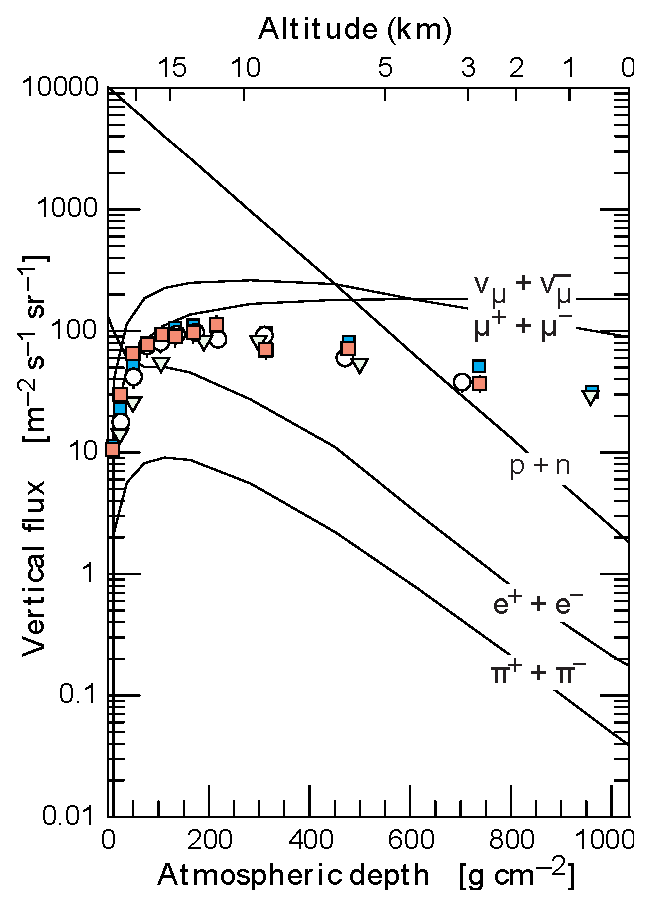
\includegraphics[width=.5\textwidth]{figures/chap2/atmospheric_cosmic_rays.eps}
	\caption[Estimated vertical fluxes of major cosmic ray components. Points are measurements of negative muons with energy larger than 1 GeV.]{Estimated vertical fluxes of major cosmic ray components. Points are measurements of negative muons with energy larger than 1 GeV.~\cite{Olive2014}}
	\label{figure:atmospheric_cosmic_rays}
\end{figure}

Daya Bay's experimental halls are also underground, and the muon-induced neutrons and isotopes constitute one of the major background sources. For Daya Bay, the sea-level muon energy and angular distribution is important because in order to get the energy and angular distribution in each hall with Monte Carlo simulation, the sea-level data, together with the mountain overburden profile and the rock composition, is input into the simulation and the muons are then propagated through the rock to get the propagated energy and angular distribution for those survived to the ceiling of the halls. Conventionally the sea-level muon flux is described by the Geisser formula~\cite{Beringer2012},
\begin{equation}
\frac{dN_\mu}{dE_\mu d\Omega}=\frac{0.14E_\mu^{-2.7}}{cm^2\cdot s \cdot sr \cdot GeV}\left\lbrace \frac{1}{1+\frac{1.1E_\mu\cos\theta}{115GeV}}+\frac{0.054}{1+\frac{1.1E_\mu\cos\theta}{850GeV}} \right\rbrace
\end{equation}
where the two terms in the braces give the contribution of pions and kaons, respectively.
  \chapter{The Daya Bay Experiment}

\section{The Daya Bay Site}
To measure $\theta_{13}$, an experimental site with reactors of high thermal power to supply large antineutrino flux and with mountains nearby to serve as cosmic ray shielding is required. Daya Bay is an appropriate site meeting the requirements.

The Daya Bay reactor complex is located on the southeast coast of China, 55 km northeast of Hong Kong. The reactor complex is composed of 3 nuclear power plants, namely the Daya Bay (DYB) nuclear power plant, the Ling Ao (LA) nuclear power plant, and the Ling Ao-II (LA II) nuclear power plant. Each nuclear power plant is equipped with a pair of functionally identical pressurized water reactors (PWR) separated by 90 m. Each reactor core supplies 2.9 GW thermal power. The last core going online started commercial operation in August, 2011. The Ling Ao nuclear power plant is \textasciitilde 1100 m from the Daya Bay nuclear power plant, and the Ling Ao-II is \textasciitilde 500 m from the Ling Ao.

The Daya Bay experimental facility is composed of 3 underground experimental halls, a surface assembly building, a liquid scintillator (LS) hall, and a water hall (EH4). The underground halls are connected by horizontal tunnels. The 3 experimental halls are where the antineutrino detectors and the muon detectors are installed. The experimental hall closest to the Daya Bay/Ling Ao nuclear power plant is called the Daya Bay/Ling Ao near site, or experimental hall 1/2 (EH1/EH2). The experimental hall farthest from all the reactor cores is called the Far site, or experimental hall 3 (EH3). The near sites are designed to hold two antineutrino detectors (ADs) each while the far site is designed to hold four ADs. The surface assembly building is the place where experimenters assemble the ADs, do the dry run tests, and other detector related work before transporting the equipment underground. The LS hall is where Daya Bay's liquid scintillator and Gd-doped liquid scintillator are produced, and is where the ADs are filled. The water hall is where the ultra-pure water system is placed which supplies ultra-pure water to the 3 water pools in EH1, EH2, and EH3. Figure~\ref{fig:dybsite} shows the experimental facility and the 6 reactor cores. The distances from the centroid of the reactor pairs to the sites are shown in Table~\ref{tab:sitecoredist}. The Global Positioning System (GPS) and modern theodolites are utilized to survey all distances. The uncertainty of the baselines from the geometric center of the reactor cores to the AD centers was determined to be about 28 mm~\cite{dayabay2012_1}.

\begin{figure}
	\centering
	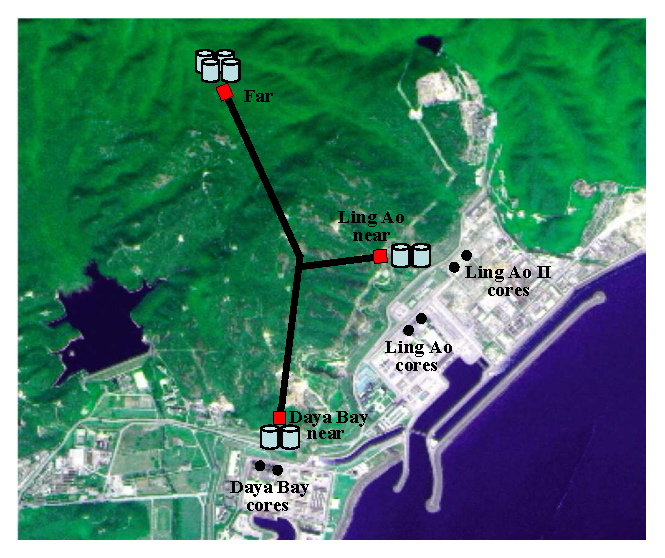
\includegraphics[width=0.45\textwidth]{figures/chap3/dayabay_site.eps}
	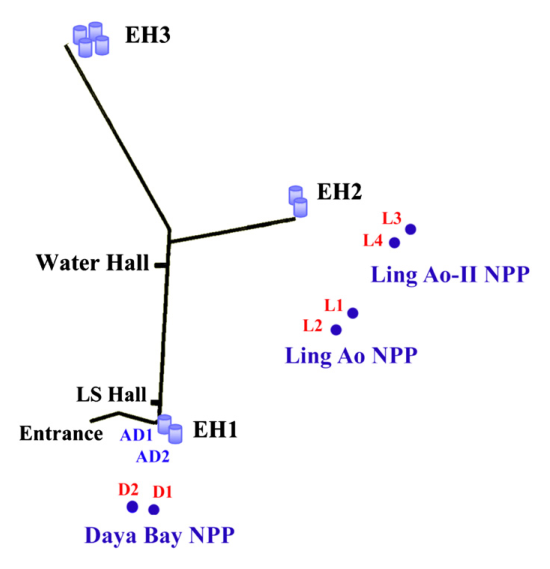
\includegraphics[width=0.35\textwidth]{figures/chap3/dayabay_site_illustration.eps}
	\caption{The Daya Bay site.}
	\label{fig:dybsite}
\end{figure}

\begin{table}
	\centering
	\begin{tabular}{|c|c|c|c|}
	\hline
	& DYB & LA & FAR \\
	\hline
	DYB cores & 363 & 1347 & 1985 \\
	\hline
	LA cores & 857 & 481 & 1618 \\
	\hline
	LA II cores & 1307 & 526 & 1613 \\
	\hline
	\end{tabular}
	\caption{Distances from the centroids of each reactor pair to the sites.}
	\label{tab:sitecoredist}
\end{table}
The overburden in equivalent meters of water (m.w.e.), simulated muon rate and average muon energy are listed in Table~\ref{table:muon_rate}.
\begin{table}
	\centering
	\begin{tabular}{cccc}
		\toprule
		& Overburden (m.w.e.) & $R_\mu$ (Hz/m$^2$) & $\left\langle E_\mu \right\rangle$ (GeV) \\
		\midrule
		EH1 & 250 & 1.27 & 57 \\
		EH2 & 265 & 0.95 & 58 \\
		EH3 & 860 & 0.056 & 137 \\
		\bottomrule
	\end{tabular}
	\caption{Vertical overburden, muon rate $R_\mu$, and average muon energy $\left\langle E_\mu \right\rangle$ of the three EHs.}
	\label{table:muon_rate}
\end{table}


\section{The Antineutrino Detector}

The antineutrino detectors (ADs) are the main detectors used for detecting neutrinos via the inverse beta decay reaction. Figure~\ref{fig:CSAD} shows the cross sectional view of the Daya Bay AD. The AD is separated into 3 different zones by 3 coaxial cylindrical vessels. From outside to inside, they are the stainless steel vessel (SSV), the outer acrylic vessel (OAV) and the inner acrylic vessel (IAV). The SSV is a 5-meter high cylinder with a 5-meter diameter. The OAV is a 4-meter high cylinder with a 4-meter diameter while the IAV is a 3-meter high cylinder with a 3-meter diameter. Inside the IAV is the neutrino target filled with 20 tons liquid scintillator (LS) doped with gadolinium (Gd). The concentration of Gd in the LS is $0.1\%$ by weight. Twenty tons of unloaded liquid scintillator is filled between the IAV and the OAV which serves as the gamma catcher. The outermost region between the IAV and the SSV is filled with 37 t of mineral oil and is call the buffer layer.
\begin{figure}
	\centering
	\includegraphics[width=0.7\textwidth]{figures/chap3/AD_cross_section.eps}
	\caption{Cross sectional view of the Daya Bay antineutrino detector.}
	\label{fig:CSAD}
\end{figure}
The gamma catcher is to capture photons leaving the target area, which relieves Daya Bay's data analysis of a fiducial volume cut which could introduce a large uncertainty. The buffer layer is to shield the target area from radioactivity in the PMTs or the SSV.
Each antineutrino detector is equipped with 192 8-inch Hamamatsu R5912 PMTs~\cite{Hamamatsu} mounted on 8 ladders along the circumference of the SSV and within the mineral oil region. The PMTs are arranged in 24 columns and 8 rings. Two specular reflectors are installed above and below the LS volume to increase the photo-coverage from 6\% to 12\%.

Three Automated Calibration Units (ACU-A, ACU-B, and ACU-C) are mounted on the top of the SSV of each AD as shown in Figure~\ref{fig:dayabay_detectors}. Each ACU contains three sources which are listed in Table~\ref{table:ACU_sources}. The sources can be deployed to better than 0.5 cm along a vertical line down to the bottom of the acrylic vessels.
\begin{figure}
	\centering
	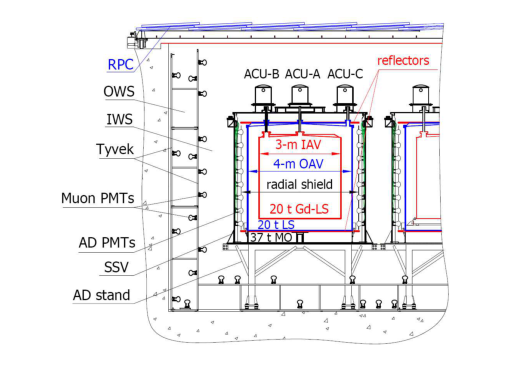
\includegraphics[width=0.7\textwidth]{figures/chap3/dayabay_detectors.eps}
	\caption{Schematic diagram of the Daya Bay detectors.}
	\label{fig:dayabay_detectors}
\end{figure}
\begin{table}
	\centering
	\begin{tabular}{ccc}
		\toprule
		source & particle & frequency (Hz) \\
		\midrule
		$^{68}$Ge & $\beta^+$ & 15 \\
		\hline
		$^{241}$Am-$^{13}$C & n & 0.5 \\
		and $^{60}$Co & $\gamma$ & 100 \\
		\hline
		LED diffuser ball & light & 500 \\
		\bottomrule	
	\end{tabular}
	\caption{Sources in an ACU and their properties.}
	\label{table:ACU_sources}
\end{table}

\subsection{The Liquid Scintillator}
Liquid scintillators (LS) usually serve as a neutrino target, and have advantages such as being cheap, easy to scale up, and easy to dope with elements. Liquid scintillators are commonly composed of two parts, the solvent and the phosphors. Aromatic organics are proven to be good solvents for LS. The electrons in the solvent molecules capture the energy of incident particles. However the solvent molecules usually have little tendency to emit light. Phosphors are added to convert the absorbed energy into light. Two classes of phosphors are usually involved in the LS, the primary scintillators and the wavelength shifters. When the solvent molecules with absorbed energy meet primary scintillator molecules, the energy gets transferred to the scintillator and light is emitted. However this light is usually in the short wavelength region, where PMTs usually have low quantum efficiency. Therefore the wavelength shifters are added to absorb and re-emit the light in the longer wavelength, usually visible light region.

Daya Bay uses linear alkylbenzene (LAB), which was also adopted by the SNO experiment, as the LS solvent~\cite{Beriguete2014}. LAB is known to have good optical transparency, in the order of 10 m, high light yield, low radioactive impurities, and high flash point for safe operation. LAB's chemical composition is basically a straight alkyl chain of 10-13 carbons attached to a benzene ring (Figure~\ref{fig:LAB}). The LS also contains 3 g/L PPO and 15 mg/L Bis-MSB as the primary scintillator and the wavelength shifter, respectively (Figure~\ref{fig:PPO} and Figure~\ref{fig:Bis-MSB}).
\begin{figure}
	\centering
	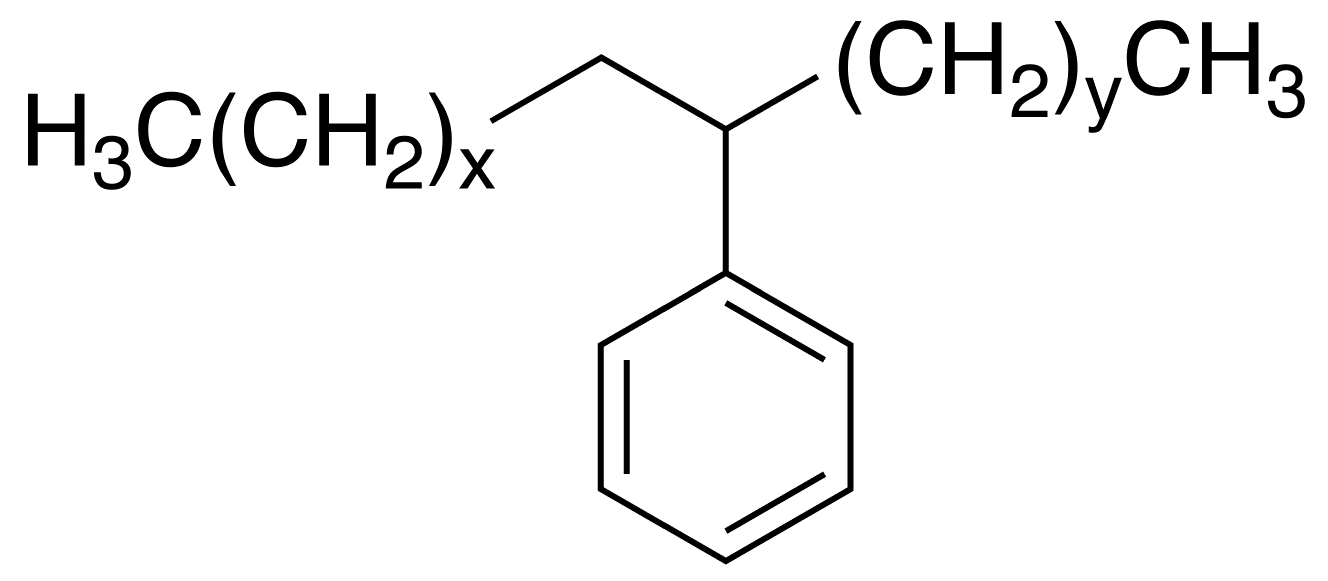
\includegraphics[width=.5\textwidth]{figures/chap3/LAB.png}
	\caption{The Daya Bay liquid scintillator solvent, linear alkylbenzene (LAB).}
	\label{fig:LAB}
\end{figure}
\begin{figure}
	\centering
  \subfloat[Primary scintillator PPO]{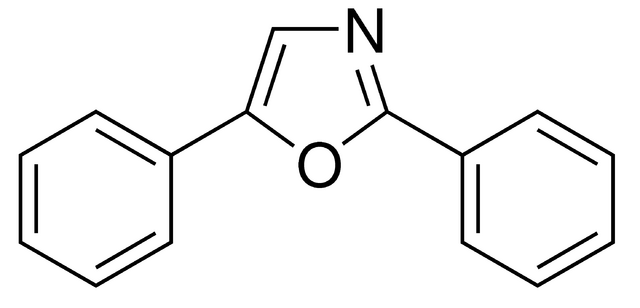
\includegraphics[height=.15\textheight]{figures/chap3/PPO.png}\label{fig:PPO}}
  \qquad
	\subfloat[Wavelength shifter Bis-MSB]{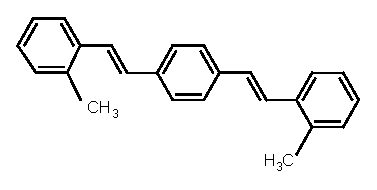
\includegraphics[height=.15\textheight]{figures/chap3/Bis-MSB.eps}\label{fig:Bis-MSB}}
	\caption{The primary scintillator and the wavelength shifter in Daya Bay's LS.}
\end{figure}

Thermalized neutrons in the scintillator can be captured on hydrogen with a mean capture time of $\sim$200 $\mu$s and decay $\gamma$'s of 2.2 MeV. The doping of gadolinium causes neutron capture on Gd with a mean capture time of $\sim$30 $\mu$s and decay $\gamma$'s of 8 MeV. The shorter capture time greatly reduces the rate of accidental coincidence, and the 8 MeV energy is way above the natural radioactivity backgrounds. Besides, the neutron capture cross section on gadolinium is 49,000 barn, more than $10^5$ times larger than the capture cross section on hydrogen ($\sim$0.3 barn). As a consequence, Daya Bay's target LS is doped with $0.1\%$ Gd.

It is seen from Figure~\ref{fig:PPO} that other than carbon and hydrogen, Daya Bay's scintillator contains other elements. Table~\ref{table:LS_composition} and Table~\ref{table:GdLS_composition} show the mass fraction of the constituent elements of the Daya Bay LS and GdLS, respectively.
\begin{table}
	\centering
	\subfloat[Mass fraction of LS]{
		\begin{tabular}{|cl|}
			\hline
			nucleus & mass fraction \\
			\hline
			C & 0.87924 \\
			H & 0.1201 \\
			O & 0.00034 \\
			N & 0.00027 \\
			S & 0.00005 \\
			\hline
		\end{tabular}
		\label{table:LS_composition}
	}
	\subfloat[Mass fraction of GdLS]{
		\begin{tabular}{|cl|}
			\hline
			nucleus & mass fraction \\
			\hline
			C & 0.87705 \\
			H & 0.12051 \\
			O & 0.00109 \\
			N & 0.00027 \\
			S & 0.00005 \\
			Gd & 0.0010315 \\
			\hline
		\end{tabular}
		\label{table:GdLS_composition}
	}
	\caption{Mass fraction of Daya Bay's LS and GdLS}
\end{table}


\section{The Muon System}

To shield the ADs from backgrounds introduced by cosmic ray muons, the ADs are surrounded by muon detectors. The Daya Bay muon system consists of two detector subsystems. One is the high-purity active water shield serving as a water Cherenkov detector in which ADs are submerged. In this study the term ``water pool'' is used interchangeably with ``water shield''. The other is the Resistive Plate Chamber (RPC) system which covers the water pool.

\subsection{The Water Cherenkov Detector}

When a charged particle passes through a medium at a speed faster than the speed of light in the medium, Cherenkov radiation is generated. Cherenkov light is detected by PMTs mounted inside the detector facing the medium. Charged particles can be detected by the Cherenkov detector with high efficiency through counting the number of PMTs receiving Cherenkov photons.

Each experimental hall has a water pool which is divided into two optically separated regions known as the inner water shield (IWS) and the outer water shield (OWS). PMTs are mounted on a support structure constructed with Unistrut and the optical separation of the inner and outer shields is achieved by a film of Tyvek~\cite{DuPont}. The number of PMTs installed in the inner and outer water shields for all sites is listed in Table~\ref{table:NPMT_water}. The inner and outer water shields operate as two independent Cherenkov detectors. The muon detection efficiency is 99.7\% and 97\% for the IWS and OWS, respectively~\cite{dayabay2012_2}.
\begin{table}
	\centering
	\begin{tabular}{cccc}
		\toprule
		& EH1 & EH2 & EH3 \\
		\midrule
		IWS & 121 & 121 & 160 \\
		OWS & 167 & 167 & 224 \\
		Total & 288 & 288 & 384 \\
		\bottomrule
	\end{tabular}
	\caption{Number of PMTs in the IWS and OWS for each site.}
	\label{table:NPMT_water}
\end{table}
In addition to acting as an active muon tagging detector, the water pool also moderates neutrons and attenuates gamma rays produced in the rock or surrounding materials in the experimental hall~\cite{dayabay2014}. Each AD is surrounded by at least 2.5 m of water in every direction. Each pool is made light-tight by covering it with a light-tight cover. The space between the cover and the water is filled with dry-nitrogen.

\subsection{The Resistive Plate Chambers}

Each water pool is outfitted with an array of RPC modules~\cite{Xu2011}. Inside the RPC modules there are RPC bare chambers which are basically parallel plate gas detectors for charged particle detection. Details of the RPC bare chmbers and the RPC modules are discussed in Chapter~\ref{chap:RPC}. In each hall the 2 m $\times$ 2 m RPC modules are laid on a support structure with edges overlapping with neighboring modules to minimize dead areas. The support structure is placed on rails, and can be retracted to provide access to the water pool. There are four layers of RPC bare chambers in each module, and each layer is associated with a readout sheet on the outside. The readout sheet is divided into strips with a width of $\sim$25 cm. The readout sheets are stacked in alternating orientation so as to reconstruct the vertex of the incident particles. The resolution of the reconstructed position is about 7 cm~\cite{Ning2013}.



%\section{The Electronics, Data Acquisition and Offline Software}
%
%For the ADs, each AD PMT raw signals are connected to the Front End Electronics boards (FEEs). Every FEE board has up to 16 channels and can do a charge integration and count for the number of PMT channels over the threshold. The system trigger can be issued by the total energy or total number of fired PMTs.
%
%Daya Bay's offline software, NuWa, is a software framework based on Gaudi which is developed at LHCb. By definition a software framework is software which provides generic functionality and in which users can add additional user's own codes to do specific jobs.
  \chapter{The Daya Bay Data Acquisition}

In this chapter the Daya Bay data processing from acquisition to analysis is introduced. First, the Daya Bay electronics is described, followed by the data acquisition and data transfer to the United States. Then Daya Bay's data quality, in particular the background due to the flasher PMTs, is discussed. After data quality the Daya Bay offline software, ``NuWa", is introduced, and the official production data are described.

\section{Trigger and Readout}
Each detector subsystem (AD, IWS, OWS, RPC) has its own readout electronics and is housed in different VME (Versa Module Europa) crates~\cite{VME1985}. VME bus is a bus system which makes use of the Eurocard standard, and is widely adopted in high energy physics experiments\footnote{For example, see \href{http://www.caen.it/csite/Product.jsp?parent=11}{the CAEN website}.}. PMT-based detectors have physically identical readout crates with the only difference in the number of PMT channels. The raw signals from PMTs are sent to the front-end electronic boards (FEEs) which sum the charge from all sixteen input channels, identify over-threshold channels, and record their timing and charge in a buffer on the board with a 40 MHz sampling rate. The FEE sends the number of channels above threshold and the sum of charges from all the channels to the trigger system. If a trigger is issued, the FEE reads out the charge and timing within 1 $\mu$s for every over-threshold channel. In the mean time the charge and timing within 100 ns just before the over-threshold instant are also read out for the electronics baseline study. There are primarily two kinds of trigger modes, the so-called NHIT mode, which counts the number of over-threshold PMTs, and the E-Sum mode, which sums the total charge of all the channels of a FEE~\cite{Gong2011}. Triggers can be issued by either mode or by requiring both. The trigger system can also accept external triggers such as those from the calibration system. The trigger system blocks triggers when either the trigger data buffer or the FEE data buffer is almost full. The blocked triggers are recorded for calculating the dead time offline.

\section{Flasher PMTs}
Daya Bay observed that a small number of PMTs emit light spontaneously, probably caused by the discharge in the PMT base~\cite{dayabay2012_2}. These are known as flasher events. For Daya Bay, the reconstructed energy of a flasher event spans a broad range, from sub-MeV up to 100 MeV. The flasher events have very distinctive signatures which can be used to reject them effectively. For one thing, the flashing PMT has a high fraction of total charge. For the other, the PMTs to the opposite side of the flashing PMT see excessive light. The charge pattern in an AD of a typical flasher event is shown in Figure~\ref{fig:flasher_charge_pattern}.
\begin{figure}
	\centering
	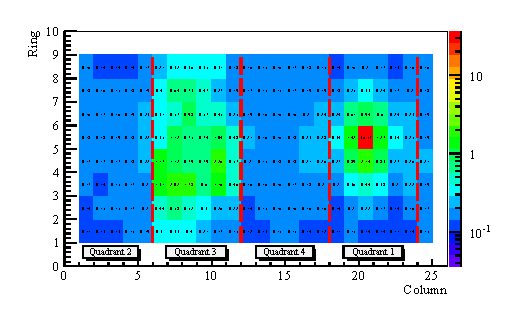
\includegraphics[width=.7\textwidth]{figures/chap4/flasher_charge_patter.eps}
	\caption{A typical flasher event with the flashing PMT in column 20 row 5 and the PMTs across the AD with high charge.}
	\label{fig:flasher_charge_pattern}
\end{figure}
To reject the flasher events, two variables are constructed, namely $MaxQ$ and $Quad$. $MaxQ$ is the largest fraction of the total detected charge seen by a single PMT. After the identification of the $MaxQ$ and the PMT corresponding to $MaxQ$, the 24 columns of PMTs are divided into four even quadrants, with the PMT with the largest charge fraction sitting in the center of the quadrant which is called Quadrant 1. Then viewed from top, the remaining quadrants are named Quadrant 2, Quadrant 3, and Quadrant 4 clockwise. The variable $Quad$ is defined as $Q_3/(Q_2+Q_4)$, where $Q_i$ is the total charge in the $i$th quadrant. It is found that the flasher events satisfy the inequality
\begin{equation}
	\left(\frac{MaxQ}{0.45}\right)^2+\left(Quad\right)^2>1
\end{equation}
The discrimination power of this cut decreases with energy. For events with values very close to $1$, careful studies are conducted, and it is found that the IBD inefficiency due to this flasher cut is $(0.02\pm 0.01)\%$~\cite{dayabay2013}. The flasher contamination in the IBD selection is estimated to be $<10^{-4}$. In addition, flasher events which survived the flasher cut would eventually be removed by the accidental background cut. Due to the high efficiency of this flasher cut, all PMTs are in operation during data taking including the flashing PMTs. In this study, all events are required to pass the flasher cut before further analysis.

\section{Data Storage and Transfer}
The raw data recorded by the DAQ system are first transferred to the Daya Bay onsite storage disks. The Performance Quality Monitoring (PQM) system~\cite{Liu2013} then uses these onsite data combined with the onsite database to produce data for online data quality check. The raw data are then transferred to the lxslc5 cluster of the Institute of High Energy Physics (IHEP) in Beijing, which in turn are transferred to the PDSF cluster of the Lawrence Berkeley National Laboratory (LBNL) for storage in the U.S.. The data route from the onsite storage to the data warehouses is shown in Figure~\ref{fig:data_transfer}.
\begin{figure}
	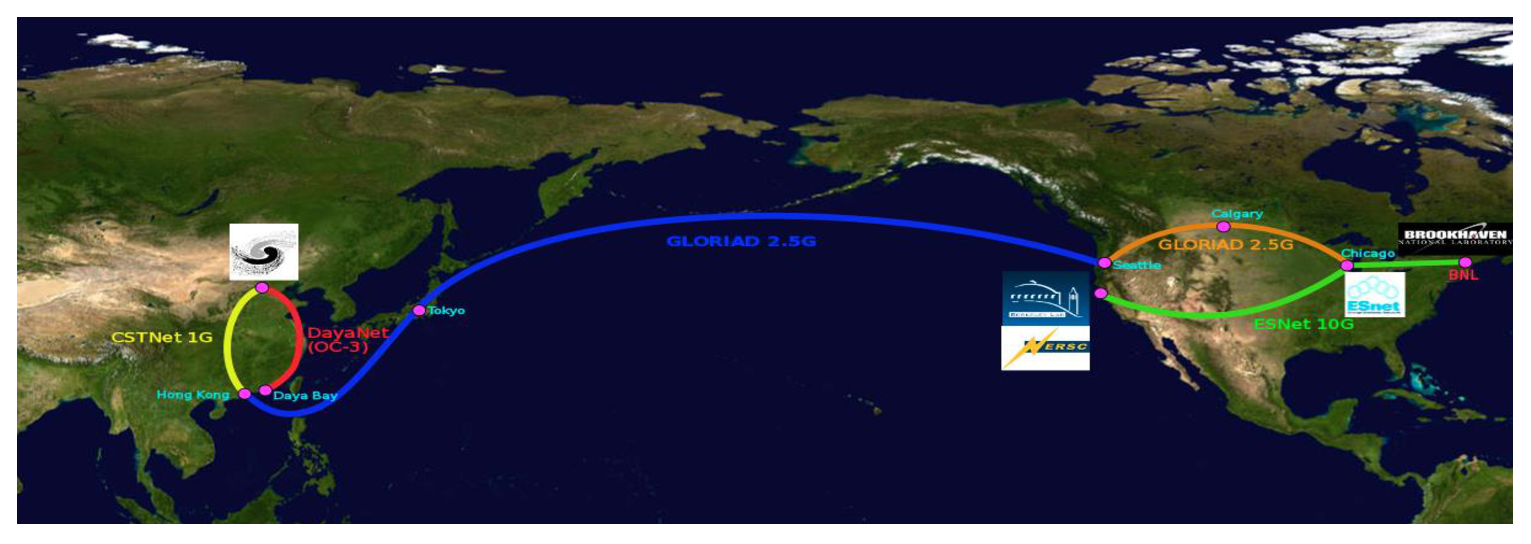
\includegraphics[width=\textwidth]{figures/chap4/data_transfer.eps}
	\caption{Data transfer from Daya Bay onsite to IHEP and from IHEP to LBNL.}
	\label{fig:data_transfer}
\end{figure}
The raw data at IHEP and LBNL are processed to produce the so called ``Keep Up Production" (KUP) data to be used by the Offline Data Monitor (ODM) system, providing offline data quality check\footnote{\href{https://portal-auth.nersc.gov/dayabay/odm}{https://portal-auth.nersc.gov/dayabay/odm}}. A Data Quality (DQ) database is constructed based on the KUP data to mark datasets with good or bad data quality.

The data transfer between the onsite and the IHEP and LBNL clusters is done with a piece of management software called SPADE. SPADE stands for South Pole Archival and Data Exchange, originally developed by IceCube and adopted by Daya Bay~\cite{docdb2696}. The design goal of SPADE is to reliably transfer data from an experiment to its data warehouse. What SPADE does is that it scans the local clusters for new files, transfers a copy to the data warehouse, and deletes the local copy. There are several advantages of employing SPADE. SPADE handles network downtime and includes bookkeeping of data movement. The adoption of SPADE by Daya Bay required only slight modifications, and SPADE has transferred Daya Bay raw data stably for years of operation.

\section{The Daya Bay Offline Software NuWa}
Daya Bay's offline software, NuWa (\textbf{N}e\textbf{u}trino at Daya \textbf{Wa}n), is a software framework~\cite{oum}. A software framework is an abstraction in which software providing specific functionality can be changed by user-written code, therefore providing application-specific software. Several key features distinguish software frameworks from libraries. The most prominent one is that the flow of control of the application is dictated by the framework instead of the user. The framework is also extensible in the sense that users can add their own code to provide specific functionality. Also the code of the framework itself is not supposed to be modified by users.

NuWa is an adaption of the LHCb/ATLAS Gaudi framework~\cite{gaudi} providing a fully developed component system for simulation, reconstruction and analysis. One important modification to Gaudi is the extension of Gaudi's Transient Event Store (TES) to Daya Bay's Archive Event Store (AES). TES is a tree (linked list) that stores all the data pertinent to the current event loop. However in the IBD analysis, not only the current event is analyzed but also the previous ones so as to form the prompt-delayed IBD coincidence. AES stores data within a user-specified time interval to resolve the problem of look-back.

Users make their own applications by writing a piece of C++ code called an ``algorithm" conforming to the requirements of the NuWa framework. Different algorithms from different authors can be cascaded to exploit the existing code. Most importantly, the adoption of software framework enables users to analyze the simulation data and the physics data with the same code.

For each data production cycle NuWa is frozen in some particular version. Before NuWa is frozen analyzers are free to add their own analysis code. After version freezing, the raw data are processed by NuWa to generate production data. The production data can be seen as ROOT trees grouped in directories. For example, the calibrated PMT hits in charge unit, the time of each PMT hit, and the RPC hit channels are all stored in the \texttt{CalibReadoutHeader} tree. The energy and vertex of each AD event, the vertex of each water pool event, and the vertex of each RPC event are reconstructed and stored in the trees in the \texttt{Rec} folder. User tagged events such as accidentals, coincidence events and muons are stored in the trees in the \texttt{Physics} folder. Table~\ref{table:production_data} lists the trees in the latest production data (P14A).
\begin{table}
	\centering
	\begin{tabularx}{\textwidth}{llX}
	\hline
	directory & tree name & use \\
	\hline
	\hline
	\texttt{\relsize{-1}/Event/CalibReadout} & \texttt{\relsize{-1}CalibReadoutHeader} & Calibrated PMT and RPC readout strip data \\
	\hline
	\texttt{\relsize{-1}/Event/Data} & \texttt{\relsize{-1}CalibStats} & Additional information for each trigger \\
	\hline
	\multirow{8}{*}{\texttt{\relsize{-1}/Event/Data/Physics}} & \texttt{\relsize{-1}ADSingles} & AD singles events outside of the muon veto window \\
	& \texttt{\relsize{-1}CoincidenceLoose} & IBD candidates with looser criteria \\
	& \texttt{\relsize{-1}CoincidenceTight} & IBD candidates with tighter criteria \\
	& \texttt{\relsize{-1}MuonData} & Muon tags \\
	& \texttt{\relsize{-1}MuonRecSimple} & Reconstructed muon track by PoolSimple and RpcSimple \\
	& \texttt{\relsize{-1}NeutronSpLoose} & Spallation neutron tags with looser criteria \\
	& \texttt{\relsize{-1}NeutronSpTight} & Spallation neutron tags with tighter criteria \\
	& \texttt{\relsize{-1}Spallation} & Muon and associated spallation neutron tags \\
	\hline
	\multirow{2}{*}{\texttt{\relsize{-1}/Event/Data/Calib}} & \texttt{\relsize{-1}Co60} & AD energy calibration data with $^{60}$Co \\
	& \texttt{\relsize{-1}Ge68} & AD energy calibration data with $^{68}$Ge \\
	\hline
	\multirow{7}{*}{\texttt{\relsize{-1}/Event/Data/Rec}} & \texttt{\relsize{-1}AdScaled} & AD energy and vertex reconstruction with $^{60}$Co \\
	& \texttt{\relsize{-1}AdSimple} & AD energy and vertex reconstruction with spallation neutrons \\
	& \texttt{\relsize{-1}AdTime} & AD vertex reconstruction with PMT timing \\
	& \texttt{\relsize{-1}AdUnfold} & AD muon track reconstruction with unfolding technique \\
	& \texttt{\relsize{-1}MuonCombined} & AD muon track reconstruction with AD PMT time and charge and RPC \\
	& \texttt{\relsize{-1}PoolSimple} & water pool vertex reconstruction with PMT charge \\
	& \texttt{\relsize{-1}RpcSimple} & RPC vertex reconstruction \\
	\hline
	\hline
	\end{tabularx}
	\caption{List of trees and uses in the production data version P14A.}
	\label{table:production_data}
\end{table}

The analysis of this study was done by writing an algorithm which fetches the geometric information of each detector and sensor (i.e. PMTs and RPC readout strips) stored in NuWa's geometric service, and uses the production data as the input data. The detailed methodology and results are presented in Chapter~\ref{chap:results}. The data analysis was done both remotely on the computing cluster at national labs and desktop computers at the University of Houston.


\subsection{Analysis on Computing Clusters}
Daya Bay has a share of the PDSF computing cluster at the National Energy Research Scientific Computing Center (NERSC)\footnote{\href{https://www.nersc.gov/}{https://www.nersc.gov/}}. PDSF is a networked distributed computing cluster designed primarily to meet the detector simulation and data analysis for large data processing projects. There are currently 2632 compute nodes available on PDSF. There is also The High Performance Storage System (HPSS)\footnote{\href{https://www.nersc.gov/users/data-and-file-systems/hpss/about/}{https://www.nersc.gov/users/data-and-file-systems/hpss/about/}} where Daya Bay stores raw and production data. The processing of the production data is done on PDSF. Any official Daya Bay collaborator has access to the CPU nodes and disk storage on PDSF.

%PDSF uses the Sun Grid Engine (SGE) as its batch system. The main instruction is \texttt{qsub}, which submits user scripts to the compute nodes in a queue until resources are granted. \texttt{qsub} can be used in array mode with a \texttt{-t} option to send a batch of similar jobs with different input at the same time. The status of a user's jobs can be checked with command \texttt{qstat}. For detailed instructions, see~\cite{SubmittingPDSFJobs}.

For a day of uninterrupted data taking, Daya Bay produces about 300 datasets of raw data. This analysis was done by sending a batch of NuWa jobs to PDSF. After processed by the user algorithm, the size of each output dataset greatly reduces from $\sim$1 GB to tens of MB. The resulting output files are then ready to undergo further analysis or generate plots.


\subsection{Analysis on Local Desktops}

High Energy Physics group at the University of Houston also has computing capacity with desktop computers with $\sim$20 cores and $\sim$20 TB storage. Since each day Daya Bay produces $\sim$300 GB of data, it is difficult to maintain a local copy of Daya Bay data more than a few days for testing analysis code. However, after data reduction on PDSF, data size is greatly reduced, and processed data can be transferred to the local computers for further analysis. The interactive jobs are much more responsive locally than remotely, and results and plots can be generated with ease locally. By this two-stage analysis method, analysis can be done efficiently, and the turnaround time between analysis iterations is shortened.
  \chapter{The RPC Muon Detector}\label{chap:RPC}

%The development of Resistive Plate Chamber (RPC) was first motivated by the need to improve detectors' timing characteristic. The first improvement was Pestov spark counter developed by Yu.N. Pestov and G.V. Fedotovich. Later on the great simplification of the realization of the concepts of Pestov counter introduced in 1981 by R. Santonico and R. Cardarelli~\cite{Santonico1981} leads to RPC. RPCs are simple in structure and cheap to manufacture, operate and scale up. RPCs have played an important role in many particle physics experiments like BaBar and LHC. The Daya Bay project also adopts the RPC as a part of the muon system.
Resistive Plate Chambers (RPCs) are planar gas detectors which have good timing resolution~\cite{Santonico1981}. RPCs are simple in structure and cheap to manufacture, easy to operate and scale up. RPCs have played an important role in many particle physics experiments BaBar, LHC, and BESIII~\cite{Han2008}. The Daya Bay project adopts the BESIII RPC as the muon top tracker.


\section{RPC bare chambers}
A RPC, called bare chamber in Daya Bay, is a parallel plate gas detector for detecting charged particles. The structure of a Daya Bay RPC bare chamber is shown in Figure~\ref{fig:rpcstruct}. A Daya Bay RPC bare chamber is formed by two 2 mm bakelite sheets~\cite{Zhang2007} separated by spacers in a 10 cm $\times$ 10 cm grid to form a 2 mm gas gap. The spacer has a disk-shaped mid-section of 12 mm to decrease the surface current.
\begin{figure}
	\centering
	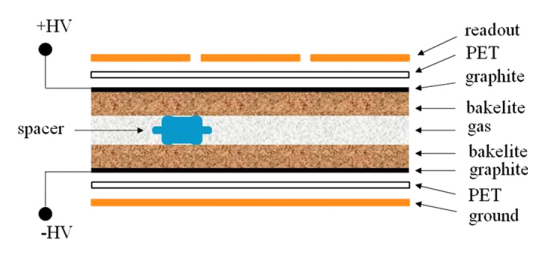
\includegraphics[width=.6\textwidth]{figures/chap5/RPC_Structure.eps}
	\caption{The structure of a Daya Bay RPC bare chamber.}
	\label{fig:rpcstruct}
\end{figure}
The total area of the button-shaped spacers occupy no more than $1\%$ of the area of a RPC bare chamber to minimize the dead area. Each bakelite sheet is coated with graphite~\cite{Ma2010} on the outside to serve as the electrode. A high voltage is applied between the two electrodes. The signal is read from readout strips from the outside. On top of the graphite there is a layer of Mylar film whose composition is polyethylene terephthalate (PET) to insulate the readout strips against the electrode and protect the graphite coating from scratching. The readout strips and ground plane are made from sheets of copper-clad FR-4. The signals are read out from the positive high voltage side.

\subsection{RPC Quality Control and Quality Assurance}
The bakelite sheets are made by Li Shen Wood Product Inc. factory in Xinji City~\cite{Ma2011}. The bakelite is made from paper soaked in phenolic and melaminic resins. The top layer is made with finer paper and melaminic coating. The error in the thickness of the sheets is within $1\%$. The length and width are about 230 cm and 120 cm. After production, the sheets were sent to IHEP, and the bulk resistivity of the sheets was measured. Four kV voltage was applied across 2 circular electrodes of 5 cm diameter, and the current was recorded to determine the resistivity. Since the measurement was done in a room without temperature control, the resistivity at 20\degree C is obtained by the following formula
\begin{equation}
	\rho_{20}=\rho_T\times 10^{0.06(T-20)}
\end{equation}
where $\rho_T$ is the resistivity measure at temperature $T$ in degrees Celsius, and 0.06 is an empirical parameter. Only bakelite sheets with resistivity in the range of 0.5-2.5 $\Omega$cm at 20 degrees Celsius are accepted and used in the module assembly. The bulk resistivity is related to the RPC performance. Higher resistivity leads to lower current and singles rate. However, when the RPC is hit by a charged particle, charges accumulate in the electrodes and then dissipate like the discharge of a capacitor. The charge in the dielectric electrodes, i.e. bakelite, follows an exponential decay $Q(t)=Q_0e^{-t/\tau}$ with a time constant $\tau=RC=\left(\rho\frac{d}{A}\right)\left(\epsilon\frac{A}{d}\right)=\rho\epsilon$, where $R$ is the resistance, $C$ is the capacitance, $d$ is the thickness, $A$ is the area, $\rho$ is the bulk resistivity, and $\epsilon$ is the permittivity of the bakelite. Therefore a larger resistivity means a longer charge relaxation time, leading to a lower detector efficiency because the area is dead. However, higher resistivity also leads to lower dark current. Since the counting rate at Daya Bay is relatively low, a higher resistivity is reasonable, but not so high as to reduce the efficiency significantly.

Bakelite sheets that passed the test were sent to Gaonengkedi Ltd. Co. (GNKD)~\cite{Ma2011} in Beijing for RPC chamber assembly. First, they were cut into 1$\times$2.1 m$^2$ and 1.1$\times$2.1 m$^2$ sheets for small and big RPCs, respectively. The size of the RPC is assured to be within $0.1\%$. A thin layer of graphite was coated on the surface of bakelite sheets, leaving 1 cm of space from the four edges. The graphite surface resistivity is required to be in the range of 400-1000 $k\Omega/\Box$. A piece of copper tape was attached to one of its corners for high voltage connection. Then a 100 $\mu m$-thick PET film covered the side of graphite coating for protection and insulation.

After the bakelite sheets were properly prepared, they were assembled into RPC chambers. First segmented edge spacers, made of the thermoplastic ABS, of size 10 mm wide and 2 mm thick, were glued along the perimeter of the bakelite sheet on the side without graphite coating. Two gas feedthroughs, also made of ABS, were embedded in the two short sides around the corners, diagonally across the sheet adjacent to the copper tape. After that the disk-shaped polycarbonate spacers were glued to the same side without graphite coating in a 10 cm $\times$ 10 cm grid, another bakelite sheet was glued on top of the spacers to form a chamber. In the first 2 hours after the chamber was sealed, the pressure in the chamber was lowered to about $8\%$ atmospheric pressure to ensure good glue cure. A $<0.1\%$ leak rate was required, and failed RPCs were glued again along the perimeter and tested again. Finally for each gas feedthrough a high voltage pin was soldered inside and made contact with the copper tape. The exposed copper tape and solder were then covered by insulating epoxy.

Newly made RPCs usually have a noise rate so high that it lowers the efficiency. It is known~\cite{ZhangJiawen2007} that a so-called training process can bring the noise down to a stable and acceptable rate. The training is done by applying the high voltage on RPC up to 10 kV for at least 48 hours, and flowing pure argon without other quenching gas so that the current can reach 2-3 orders of magnitude higher than that of normal operation condition. The training process burns off dust and ``polishes'' the surfaces. Figure~\ref{fig:training_current} shows the training current of a sample of 7 RPCs.
\begin{figure}[ht]
	\centering
	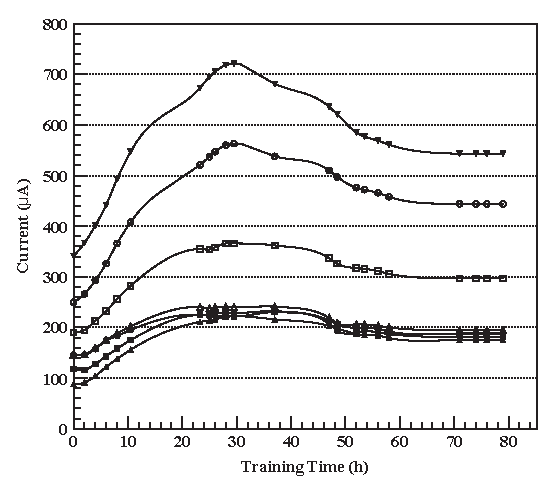
\includegraphics[width=.7\textwidth]{figures/chap5/training_current.eps}
	\caption{Training current of 7 RPCs.}
	\label{fig:training_current}
\end{figure}
We see that the current rises in the beginning and then drops off to a steady value. After training, when the RPC is put to use and operated in normal condition, the current is usually reduced by a factor of 10 compared with RPCs which are not trained.

%A gas combination of Ar, isobutane and R-134A flows in the gap. When charged particles pass through the gas gap, Ar molecules are ionized and the released electrons then undergo acceleration by the applied electric field. This primary electron then ionizes other Ar molecules and generates an electron avalanche. When the avalanche electrons drift the the anode, they induce electric signals which can then be readout. The isobutane can absorb ultraviolet photons and prevents a secondary streamer. The R-134A has high electron affinity and can restrict the size of the streamer.


\section{RPC Modules}
The RPC arrays in EH1 and EH2 are composed of 6 rows $\times$ 9 columns of RPC modules while that in EH3 is composed of 9 rows $\times$ 9 columns of RPC modules. Each module is an aluminum box of dimensions 2.17m $\times$ 2.20m $\times$ 0.08m containing bare chambers, insulating materials, support panels, readout strips, and ground planes. The RPC modules sit on the support structure which can be moved to an ``RPC hall'' next to the water pool during the AD and water pool installation. At each site, two additional RPC modules are installed at two opposing sides of the water pool, around two meters above the RPC array. Figure~\ref{fig:support_structure} shows the arrangement of the RPC modules on the support structure and the axes for defining the rows and columns of a RPC module.
\begin{figure}
	\centering
	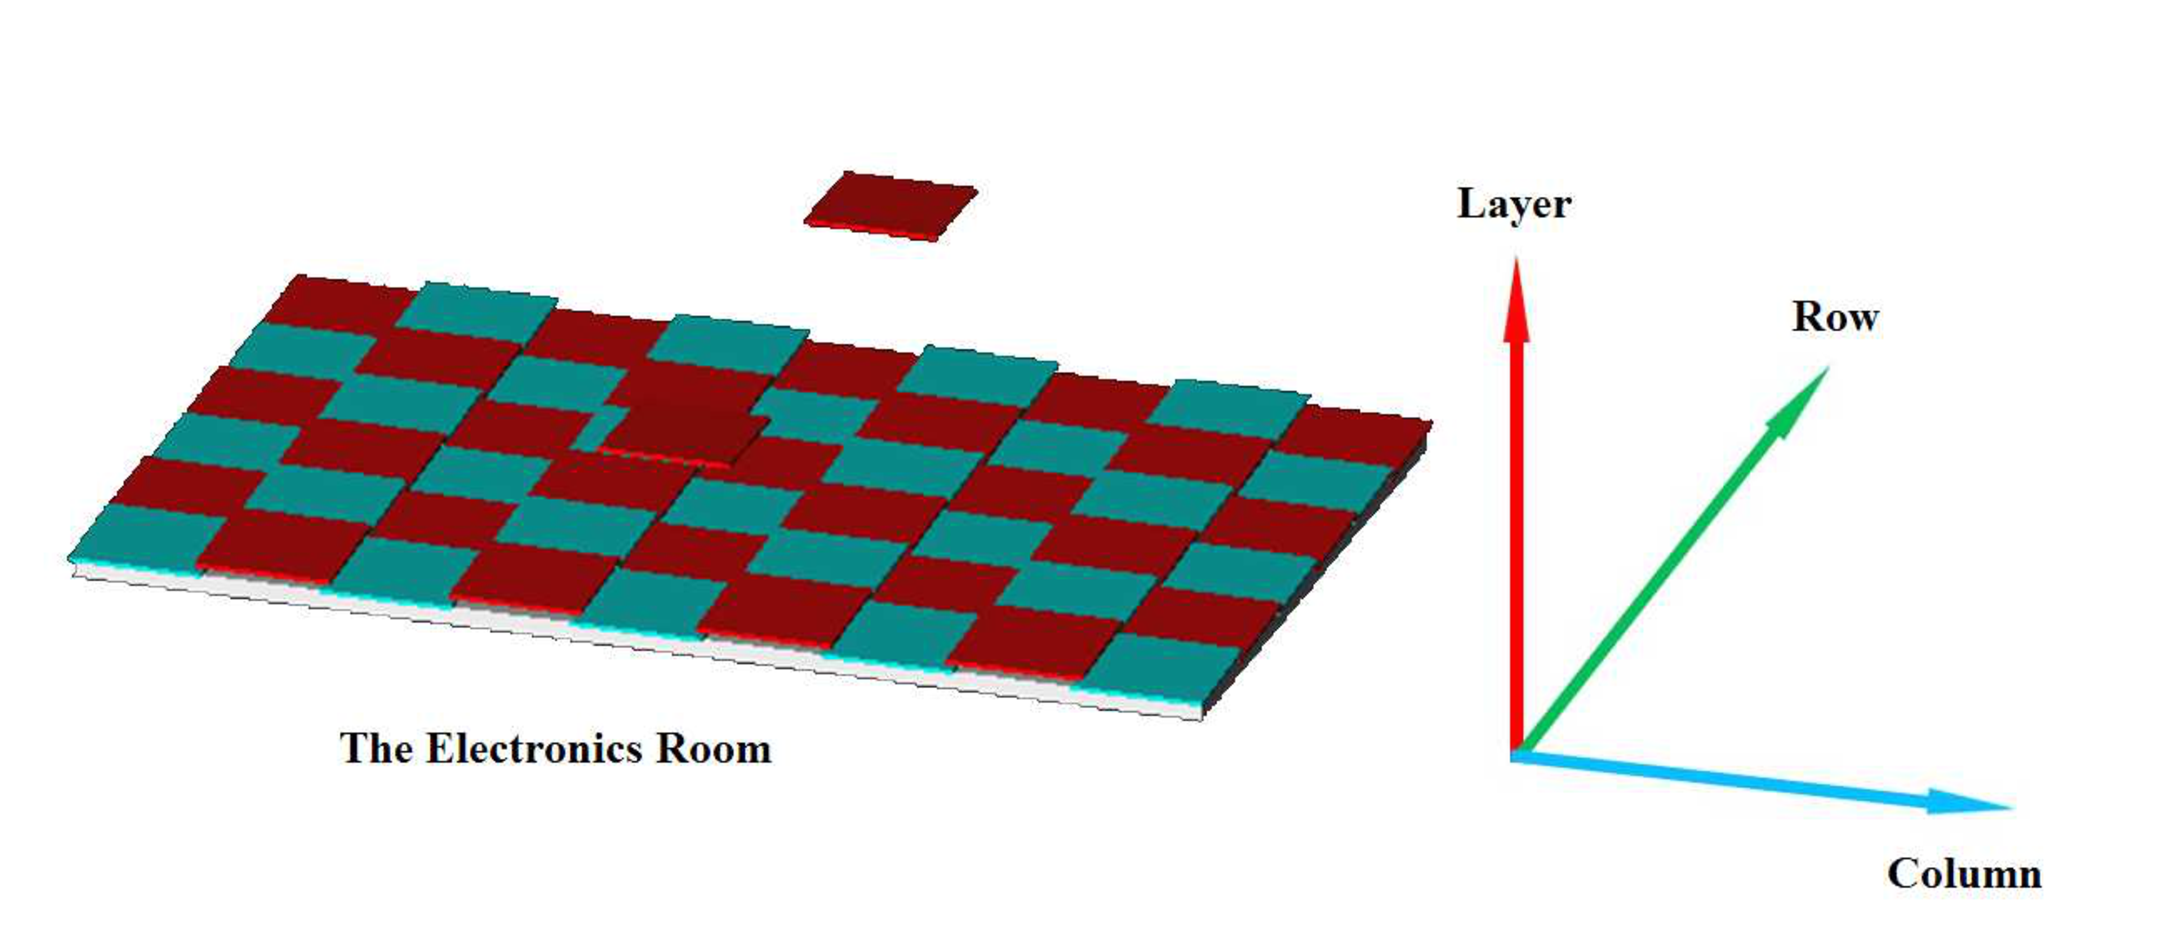
\includegraphics[width=0.7\textwidth]{figures/chap5/support_structure.eps}
	\caption{The arrangement of the RPC modules on the support structure and the convention used for locating a RPC module.}
	\label{fig:support_structure}
\end{figure}
Note that there is a 10 cm overlap on all sides of adjacent modules aiming at minimizing the dead regions. The inner structure of a Daya Bay RPC module is shown in Figure~\ref{fig:module_inner_structure}.
\begin{figure}
	\centering
	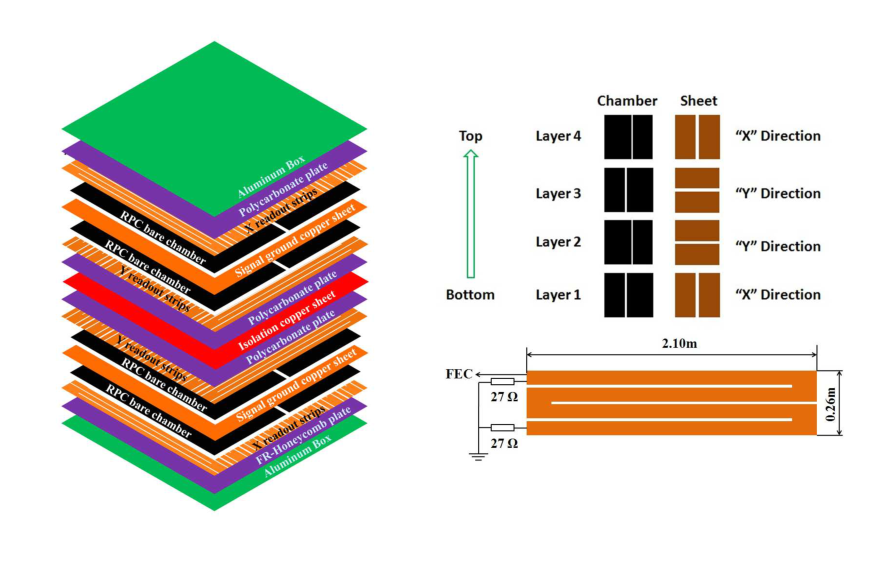
\includegraphics[width=0.9\textwidth]{figures/chap5/RPC_inner_structure.eps}
	\caption{Left: the inner structure of a RPC module. Right: the arrangement of RPC bare chambers for each layer and the zigzag structure of a readout strip.}
	\label{fig:module_inner_structure}
\end{figure}
A RPC module is composed of 4 layers of RPC bare chambers. Each layer is formed by 2 RPC bare chambers with the same length but different width. The larger RPC bare chamber has a dimension of 2.1 m $\times$ 1.1 m. The smaller one has a dimension of 2.1 m $\times$ 1.0 m. From bottom to top, the sizes of the RPC bare chambers alternates so as to offset the dead region due to the edges of the bare chambers. Each RPC layer is equipped with a 2.1 m $\times$ 2.1 m copper-clad FR-4 readout plane consisting of 8 readout strips resulting in a strip dimension of 26 cm $\times$ 210 cm. The strips are of a zigzag design which is equivalent to a strip 6.5 cm wide and 8.4 m long (see bottom right of Figure~\ref{fig:module_inner_structure}). The zigzag design in effect changes the impedance so as to give a larger and narrower pulse because of the change in the impedance of the transmission line~\cite{Riegler2002}. One end of the strip is connected to the RPC Front End Card (FEC, see Section~\ref{sec:RPC_electronics}) while the other end is connected to a ground by two 27 $\Omega$ resistors, a value determined in bench tests (see Figure~\ref{fig:RPC_signal}(a)). Figure~\ref{fig:RPC_signal}(b) shows some signals read out by the oscilloscope in bench tests. The signal threshold in Daya Bay's physics data taking is set at 30 mV.
\begin{figure}
  \centering
  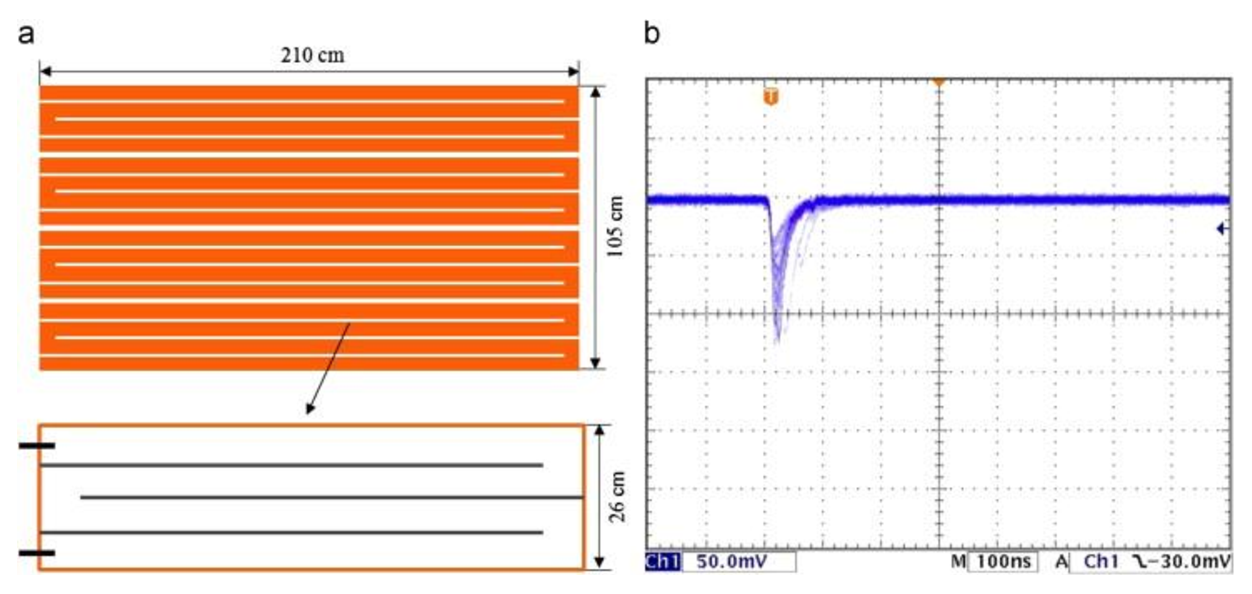
\includegraphics[width=0.8\textwidth]{figures/chap5/RPC_signal.eps}
  \caption{(a) Readout zigzag structure and the signal termination. (b) Readout signals on the oscilloscope.}
  \label{fig:RPC_signal}
\end{figure}
The 4 readout layers are oriented, from bottom to top, in the $x$, $y$, $y$, $x$ directions as shown in Figure~\ref{fig:module_inner_structure}. With this readout arrangement, the position of the incident muon can be determined by identifying the intersection of the $x$ and $y$ strips.


\section{Gas and High Voltage System}
The RPCs operate in streamer mode with a gas mixture of Ar:C$_2$H$_2$F$_4$:i-C$_4$H$_{10}$:SF$_6$=65.5:30:4:0.5. Each site has a gas system which consists of gas cylinders, gas mixing and distribution systems, fire safety monitoring systems, and gas chromatography (GC) systems. The flow rate of each site is about 1 RPC volume exchange per day, and is controlled by an electronic mass flow control system.

The high voltage (HV) system includes a CAEN HV mainframe for supplying the operating 7600 V HV, the fanout boxes for HV channel multiplication, and the HV interface boxes for connecting the HV to the RPC module. The HV channels from the mainframe are controlled and monitored remotely by the Daya Bay Detector Control System (DCS). There is also an interlock functionality to ensure safe operation: if there are alarm signals from the gas system, the HV DCS sends out warnings to the monitors in the control room, and allows 30 minutes for troubleshooting before the HV gets automatically shut down.


\section{RPC Readout Electronics}\label{sec:RPC_electronics}
Figure~\ref{fig:RPC_electronics} shows the architecture of the RPC readout electronics. The readout system consists of four boards and modules, namely the Front-End Card (FEC), the ReadOut Transceiver (ROT), the ReadOutModule (ROM), and the RpcTroggerModule (RTM). The number of each kind of board or module installed in each hall is summarized in Table~\ref{table:num_installed}.
\begin{figure}
	\centering
	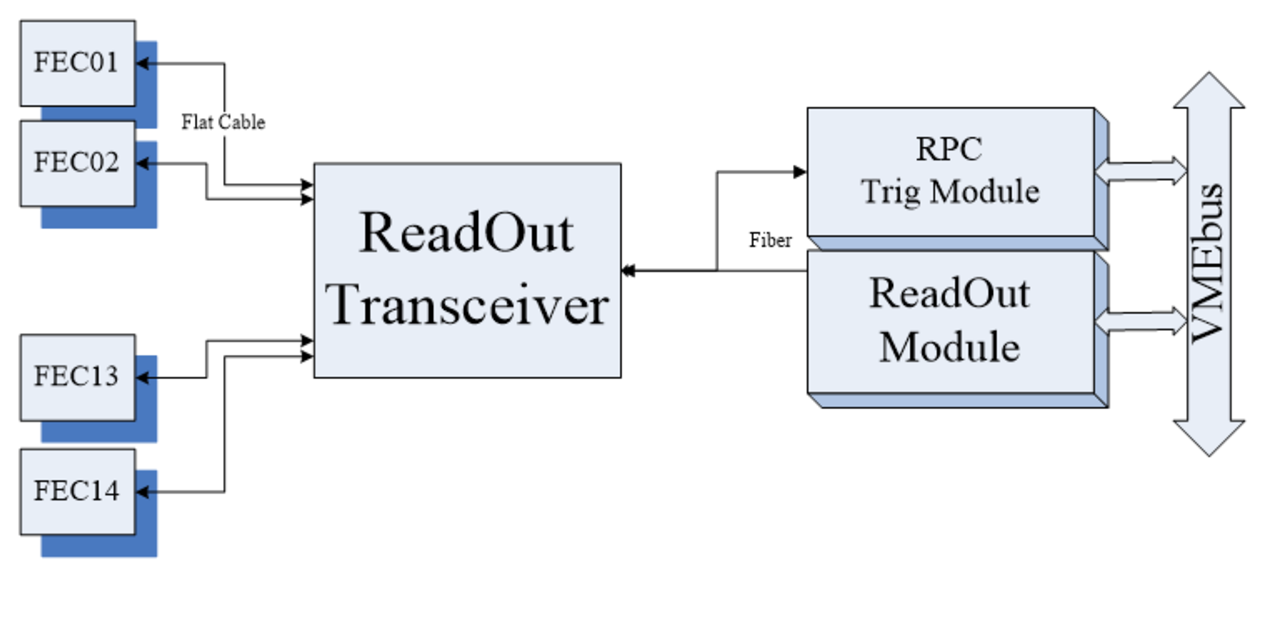
\includegraphics[width=.75\textwidth]{figures/chap5/RPC_Readout.eps}
	\caption{Architecture of the RPC readout electronics.}
	\label{fig:RPC_electronics}
\end{figure}
\begin{table}
	\centering
	\begin{tabular}{ccc}
		\hline
		board or module & near hall & far hall \\
		\hline
		FEC & 54 & 81 \\
		ROT & 4 & 6 \\
		ROM & 1 & 1 \\
		RTM & 1 & 1 \\
		\hline
	\end{tabular}
	\caption{Number of boards/modules installed in each hall.}
	\label{table:num_installed}
\end{table}
Daya Bay's FEC is the signal front end readout card for RPC detectors. Each card collects signals from the 32 channels of a RPC module. The FEC amplifies the signal, and generates a digital signal for signals above 30 mV threshold, and adds timestamp from the system clock. FECs generate local triggers with different modes specified by input signals and pass them to ROT. Signal transmission from FEC to ROT is done with flat cables. There are two kinds of local trigger modes, 2/4 and 3/4. In 2/4 mode, triggers are issued if at least two layers of RPCs are fired. In 3/4 mode, triggers are issued if at least three layers of RPCs are fired. In Daya Bay's physics data taking, since the amount of data generated by 2/4 mode takes too much storage and is mostly due to non-physics events, 3/4 trigger mode is used.
The ROT transmits readout data and configuration data between FEC and ROM. In addition, ROT transmits local trigger signals to RTM. Each ROT accepts up to 15 FEC signals, packs up data from 15 cards, and passes them to ROM and RTM through optical links. The ROM and RTM then process the data and issue triggers.


\section{Event Reconstruction}
In this study the yield of muon-induced neutrons is measured by constructing fiducial volumes around the muon tracks. Only neutrons captured inside the fiducial volume are counted. In this section the event vertices and the muon tracks are discussed.

\subsection{AD Event Reconstruction}
In this study, the energy and vertex of an AD event are obtained by the ``AdSimple'' reconstruction algorithm~\cite{docdb7334}. AdSimple reconstructs the energy and vertex of a point-like event such as the neutron capture on Gd.
\paragraph{Vertex Reconstruction} The vertex reconstruction in AdSimple involves two steps. First the charge-weighted mean from all PMTs is used to obtain the preliminary value. Then a correction scheme obtained from MC simulation is applied to the preliminary value.
The preliminary vertex is obtained by
\begin{equation}
	\vec{r}_{coc}=\frac{\sum\limits_iQ_i\vec{r}_i}{\sum\limits_iQ_i}
\end{equation}
where $\vec{r}_{coc}$ is the center of charge position, $i$ runs over all 192 8" PMTs, $Q_i$ is the charge received by the $i$th PMT, and $\vec{r}_i$ is the position of the PMT.
As a result of reflectors on the top and bottom of the AD, it is found that the the center of charge positions $\vec{r}_{coc}$ are pulled to the center of the AD. This bias can be corrected by the IBD Monte Carlo simulation including both positron and neutron events. The OAV is divided into bins in both the radial $\rho$ and the vertical $z$ directions. Then quantities $\Delta \rho$ and $\Delta z$ are defined\footnote{\begin{eqnarray}
\Delta \rho &=& \vec{\rho}_{true}\cdot \frac{\vec{\rho}_{coc}}{\rho_{coc}}-\rho_{coc} \\
\Delta z &=& z_{true}-z_{coc}
\end{eqnarray}} representing the deviation of $\vec{r}_{coc}$ from the true position $\vec{r}_{true}$. For each bin the average values of $\Delta \rho$ and $\Delta z$ are calculated, and these values are assigned to the center of the bin. To obtain $(\Delta\rho,\Delta z)$ for all $(\rho,z)$, an interpolation is applied. Finally the correction is added to each $\vec{r}_{coc}$ to obtain the reconstructed vertex $\vec{r}_{rec}$. The position resolution of this algorithm for Gd captured neutrons is $\sim$20 cm in both $\rho$ and $z$ directions.

\paragraph{Energy Reconstruction} The AdSimple energy reconstruction involves three steps. The first step is the determination of the total charge deposited in the detector recorded by PMTs. The second step is the conversion of this charge to a physical energy scale. \mbox{Finally}, a correction is applied to account for the detector non-uniformity.
Concerning the total charge determination, for an AD trigger the energies deposited in all PMTs are all counted. For each PMT, the pedestal subtracted ADC value is converted into number of photoelectrons (pe's) using the calibration constants specific to individual channels in the offline database which is updated weekly. Only PMT hits in the time window $[-1650ns,-1250ns]$ with respect to the time the trigger is issued are summed to obtain the PMT charge for each PMT.
%The reason is that if all PMT hits in a readout are used, it will give a worse energy resolution due to the inclusion of too many dark hits or afterpulses.

Once the total charge sum is obtained for an AD trigger in the units of photoelectrons, the charge has to be converted into real physical energy scale. Here the spallation neutrons are used to set the photoelectron to energy scale. The spallation neutrons captured on Gd is uniformly distributed in the GdLS, providing access to the whole detector active volume. The 8 MeV peak is close to the lower bound of the delayed signal energy cut which constitute a dominant systematic uncertainty. The number of photoelectrons divided by 8 MeV then serves as the energy scale constant for the AD. For all ADs, this value is about 170 photoelectrons/MeV. Finally the energy scale as a function of $r$ and $z$ are studied and corrected.

In this study, muon-induced neutrons are selected by an energy cut with energies reconstructed by AdSimple algorithm. Also, the capture sites of neutrons are required to be within a fiducial volume with capture vertices reconstructed by this algorithm as well.

\subsection{Muon Track Reconstruction}
In this study, muon tracks are reconstructed by the muon system. The muon system consists of three independent detectors, the RPC, the IWS, and the OWS. The RPC by design can reconstruct the muon incident position simply by identifying the intersection of the fired strips which gives a point in the muon track. On the other hand, the two PMT-based Cherenkov detectors can each offer an reconstructed point in the muon track by the PMT charge pattern. Thus, from the muon system alone, at most four points can be obtained if the muon passes through the telescope RPC, the RPC array, the IWS, and the OWS. A muon track can be reconstructed utilizing those points reconstructed with the individual muon subsystems.

\subsubsection{RPC Vertex Reconstruction}
RPC readout strips by design are used for muon point reconstruction. Since in the physics data taking the 3/4 trigger scheme is used, there is at least a pair of $x$ and $y$ strips from adjacent layers, cf. Figure~\ref{fig:module_inner_structure}. The eight $x$ strips and the eight $y$ strips divide the surface of a RPC module into 64 ``patches''. One can then assign the coordinate of the center of the patch formed by the fired strips as the reconstructed point. Figure~\ref{fig:RPC_event} is an example of a real RPC event. If in the same readout layer several contiguous strips, which we call clusters, are fired, the centroid of them is used. If two layers with the same strip orientation, say the $x$ layers, contain fired strips, the centroid of the layer centroids is used as the reconstructed coordinate.
\begin{figure}
	\centering
	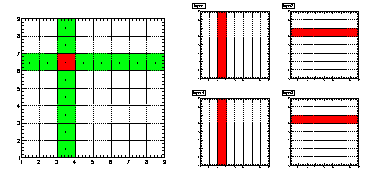
\includegraphics[width=0.9\textwidth]{figures/chap5/RPC_event.pdf}
	\caption{A RPC event. Left: multiplicity of fired patches. Right: fired strips in each layer.}
	\label{fig:RPC_event}
\end{figure}

Some rarer situations have to be considered here. If in the same layer several disjoint clusters exist, ``ghost hits'' are formed, i.e., there are multiple intersection points of $x$ and $y$ clusters. For Daya Bay, it is difficult to discriminate ghost hits from real hits. Fortunately the fraction of events with ghost hits is very small. There are also crosstalk events due to strong signals penetrating the copper ground plane in the center of the module. For such kind of events, most strips ($>4$) in the central two $y$ layers have hits. To remove the crosstalk events, a simple cluster size cut with at most two contiguous strips removes them effectively. Based on one day of data, the approximate distributions of the RPC hit pattern are
\begin{itemize}
	\item 97\% of the clusters are of size 1 strip,
	\item 96\% of the triggers contain only 1 muon per module,
	\item 97\% of the triggers contain only 1 module in the entire hall,
	\item 99\% of the events fire vertical clusters.
\end{itemize}
From these distributions we see that the RPC muon detector in fact serves as a high efficiency ($>95\%$~\cite{Ning2013}), low noise muon tracking detector.

\subsubsection{Water Shield Vertex Reconstruction}
The algorithm for water pool vertex reconstruction is dubbed ``PoolSimple''~\cite{docdb7838}. The water shields detect relativistic charged particles through the emission of Cherenkov radiation when the speed of the charged particle is larger than the speed of light in water. Unlike the uniform emission of scintillation light produced by the AD events, the Cherenkov photons are emitted in a cone relative to the direction of the charged particle. For water, this angle is about 41\textdegree. A complete water Cherenkov reconstruction algorithm should employ the timing information of PMT hits. However, getting the timing calibration done correctly is a rather involved task and the current preliminary results~\cite{docdb7696} still have room to improve. This algorithm uses only the PMT charge and hit pattern to reconstruct the muon track, and it turns out to have a reasonably good resolution.

As in the AD vertex reconstruction, a charge-weighted mean is used as the reconstructed vertex,
\begin{equation}
	\vec{r}_{rec}=\frac{\sum\limits_{i=1}^{n_{max}}Q_i\vec{r}_i}{\sum\limits_{i=1}^{n_{max}}Q_i}
\end{equation}
where $Q_i$ is the charge the $i$th PMT receives, and $\vec{r}_i$ is the position vector of that PMT. $n_{max}$ is the first $n_{max}$ PMTs with the largest received charge, and is determined by simulation. The idea is that the closer the PMT is to the muon track the more light it will receive. Also since the Cherenkov radiation is directional, the PMTs in proximity to the PMT with largest charge receive more light than PMTs far from the muon track. Therefore only selecting a number of PMTs with the largest charge provides better resolution than taking all PMTs in the pool. Since each water pool is regarded as an independent detector, this algorithm gives two reconstructed vertices, one for each pool.

The resolution of this algorithm is obtained by simulation. One can determine the distance from the center of the OWS to the true track. Call this parameter $d_{true}$. The same point to the reconstructed track is $d_{rec}$. One can plot the distribution of $d_{rec}-d_{true}$. The position resolution obtained from the distribution is $\sim$60 cm shown in Figure~\ref{fig:WS_resolution}.
\begin{figure}
	\centering
	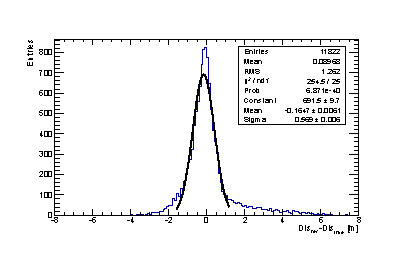
\includegraphics[width=0.7\textwidth]{figures/chap5/WS_resolution.eps}
	\caption{The distribution of $d_{rec}-d_{true}$.}
	\label{fig:WS_resolution}
\end{figure}

\subsubsection{Muon Track Reconstruction}
When a muon passes through the Daya Bay muon system, depending on the geometry of the track and the muon detectors, at most four points can be reconstructed if the telescope RPC is also hit by the muon. Since RPCs have a superior resolution than the water pool, in this study only muons having an RPC trigger and a water pool vertex are considered. Furthermore, since ADs are sitting in the inner water pool, the PMTs on the bottom of the pool are shadowed by the ADs. This situation known as the AD shadowing effect. The result is that the bottom PMTs don't see enough light, pulling the reconstructed vertex towards the wall of the water pool. Contrarily, the outer water pool doesn't suffer from this effect. Consequently, the muon track used in this study is obtained by connecting the RPC and the OWS vertices.
  \chapter{Neutron Production Mechanisms in Liquid Scintillator}\label{chap:yield_theory}

Muons interact with matter through the exchange of virtual photons. The nuclei get excited by the virtual photons, and when they de-excite, neutrons can be released. Neutrons generated by the muon-nucleus interactions are called directly generated neutrons. Electromagnetic fields produced by charged particles can be thought of as a swarm of virtual photons traveling with the particles. When a muon passes by an atomic nucleus, it interacts with the nucleus by exchanging virtual photons with the nucleus. The Feynman diagram for the virtual photon interaction with the nucleus is shown in Figure~\ref{fig:muon_spallation}.
\begin{figure}
	\centering
	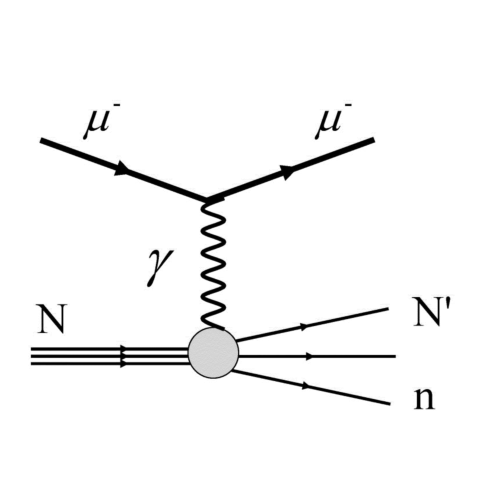
\includegraphics[width=.5\textwidth]{figures/chap6/mu_N_Feynman_diagram.eps}
	\caption{Feynman diagram of muon-nucleus interaction by exchange of a virtual photon.}
	\label{fig:muon_spallation}
\end{figure}
To quantify direct neutron generation, one can first get the virtual photon frequency spectrum with Williams-Weissacker's method of virtual quanta, and then fold it with the photonuclear total cross section of the material under study. The total cross section of the muon-nucleus interaction can then be written as~\cite{Formaggio2004}~\cite{Luu2006}
\begin{equation}\label{eq:mu_N_cross_section}
	\sigma_{\mu N}=\int\frac{n_\gamma(\nu)\sigma_{\gamma N}(\nu)}{\nu}d\nu
\end{equation}
where $n_\gamma(\nu)$ is the virtual photon spectrum associated with the passing muon, $\nu$ is the photon energy, and $\sigma_{\gamma N}(\nu)$ is the real photonuclear cross section. The virtual photon spectrum can be written as~\cite{Delorme1995}
\begin{equation}
	n_\gamma(\nu)=\frac{\alpha}{\pi}\left[\frac{E^2+E'^2}{P^2}\ln\frac{EE'+PP'-m_\mu^2}{m_\mu\nu}-\frac{(E+E')^2}{2P^2}\ln\frac{(P+P')^2}{(E+E')\nu}-\frac{P'}{P}\right]
\end{equation}
where $\alpha$ is the fine structure constant, and $E(E')$ and $P(P')$ are the energy and momentum of the muon before(after) interaction, respectively. The photonuclear cross section was measured by various experiments. Consequently, the cross section of the muon-nucleus interaction can be obtained by Equation~\ref{eq:mu_N_cross_section}. The average number of neutrons $\bar{N}_n$ produced through muon-nucleus interaction by a muon traversing a distance $\ell$ is
\begin{equation}
	\bar{N}_n=n_T\left\langle f\sigma_{\mu N} \right\rangle\ell
\end{equation}
where $n_T$ is the number of target nuclei per unit volume, $f$ is the neutron multiplicity, $\sigma_{\mu N}$ is the muon-nucleus interaction cross section, and $\ell$ is the distance the muon traverses in the medium. The real photon interacts with the nucleus through different mechanisms at different photon energies, and produces a different mean number of neutrons. Thus, when convoluting the virtual photon spectrum with the real photon cross section, different mechanisms have to be considered in accordance with the photon energy. In the order of increasing energy, the dominant processes are giant dipole resonance (GDR) and the $\Delta$ resonance production. Figure~\ref{fig:photo_absorption} shows the photo-absorption cross section of carbon, the dominant element of the liquid scintillator. The peak around 20 MeV corresponds to the GDR and the peak at 300 MeV corresponds to the $\Delta$ production. Figure~\ref{fig:virtual_photon_flux} shows the virtual photon flux $\frac{n_\gamma(\nu)}{\nu}$ for a 100 GeV muon, and Figure~\ref{fig:photonuclear_cross_section} shows the real photonuclear interaction cross section with $^{12}$C from various measurements~\cite{Kossov2002}. Note that $\sigma_{\mu N}$ is the product of the two functions (cf. Figure~\ref{fig:folded_cross_section}), which greatly suppresses the high energy processes due to the deep inelastic scattering.
\begin{figure}
	\centering
	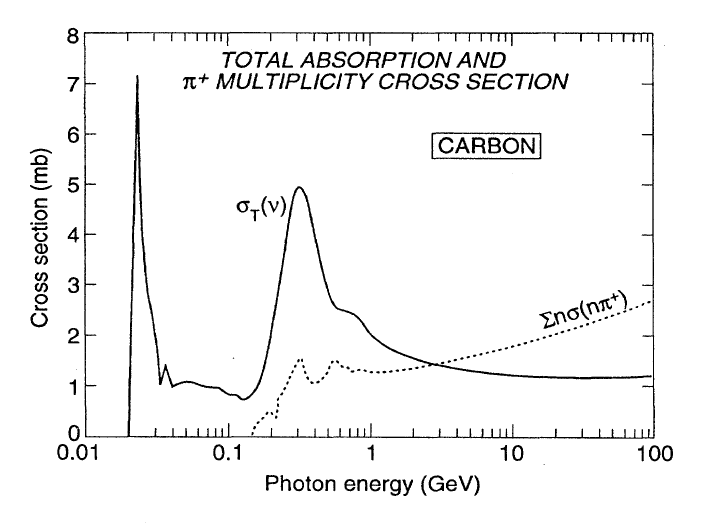
\includegraphics[width=.7\textwidth]{figures/chap6/photo_abroption.png}
	\caption{Solid line shows the photo-absorption cross section of carbon.}
	\label{fig:photo_absorption}
\end{figure}
\begin{figure}
	\centering
  \subfloat[$\frac{n_\gamma(\nu)}{\nu}$]{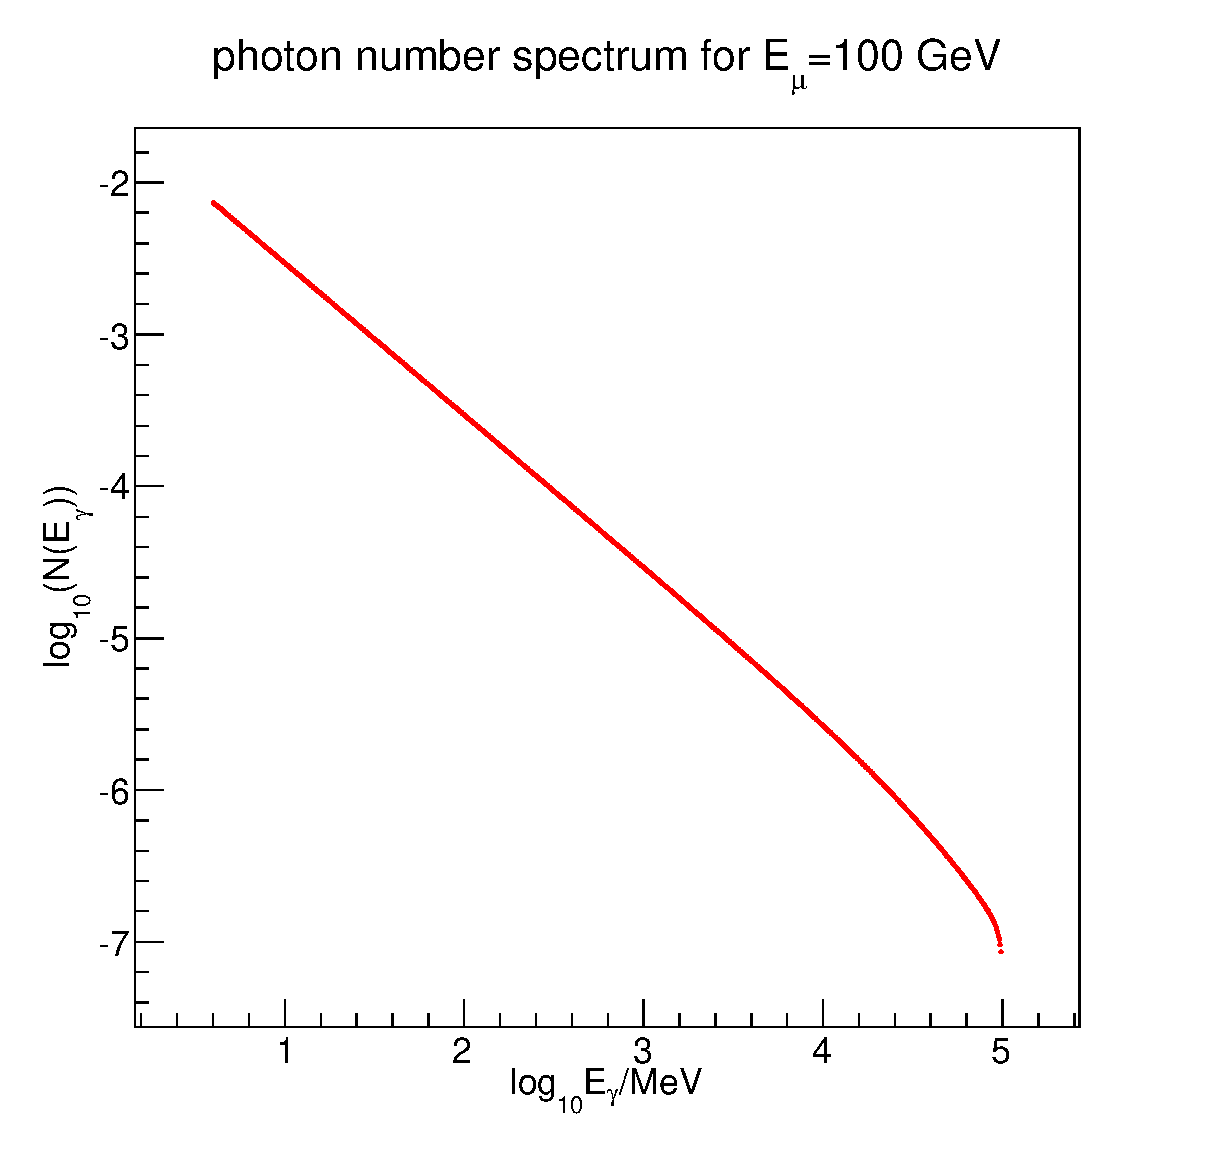
\includegraphics[height=.25\textheight]{figures/chap6/loglog.eps}\label{fig:virtual_photon_flux}}
  \qquad
	\subfloat[photonuclear interaction cross section]{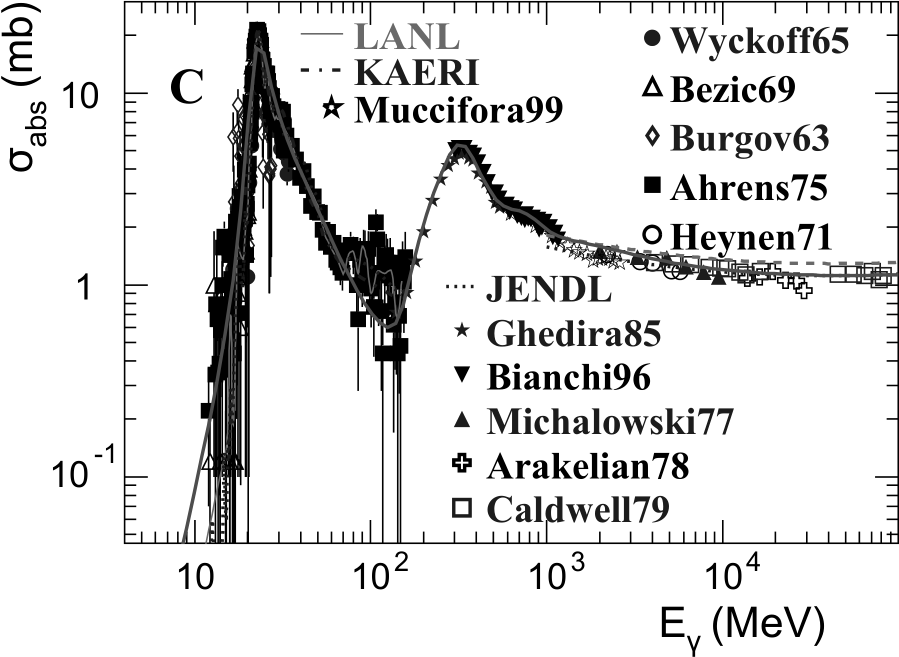
\includegraphics[height=.25\textheight]{figures/chap6/photonuclear.png}\label{fig:photonuclear_cross_section}}
	\caption{The virtual photon flux for a 100 GeV muon and the real photon interaction cross section. The muon nucleus interaction cross section is the product of the two functions.}
\end{figure}

\paragraph{Giant Dipole Resonance}
In the photonuclear interaction cross section, the process taking place with the lowest energy is giant dipole resonance. When photons with wavelength comparable to the size of the nucleus, they see the nucleus as a whole. The oscillating electric field displaces the protons away from their equilibrium position, and an electric dipole is formed. When the giant dipole is formed, the nucleus is in excited state, and when the nucleus de-excites, one or more neutrons can be released. At low photon energies (below $\approx 30$ MeV), photon absorption is dominated by GDR, which decays occasionally by neutron emission~\cite{Bortignon1998}. Table~\ref{table:GDR_carbon}~\cite{IAEALib} shows the threshold energies for different final state particles of the photonuclear reaction with $^{12}$C. This table shows that four decay modes involve at least one neutron in their final states. This indicates the neutron multiplicity of the GDR decay may be larger than one.
\begin{table}
	\centering
	\begin{tabular}{cccccccccc}
	\hline
	Abundance & \multicolumn{9}{c}{Threshold Energies (MeV)} \\
	($\%$) & $\gamma,n$ & $\gamma,p$ & $\gamma,t$ & $\gamma,^3$He & $\gamma,\alpha$ & $\gamma,2n$ & $\gamma,np$ & $\gamma,2p$& $\gamma,3n$ \\
	\hline
	98.89$\%$ & 18.72 & 15.96 & 27.37 & 26.28 & 7.37 & 31.84 & 27.41 & 27.19 & 53.13 \\
	\hline
	\end{tabular}
	\caption{The threshold energies and the released particles for the photonuclear reaction of $^{12}$C.}
	\label{table:GDR_carbon}
\end{table}


%\paragraph{quasideutron}
%With higher photon energy, the photons start to see the proton-neutron pair in the nucleus.


\paragraph{$\Delta$ production}
$\Delta$ resonances are excited states of nucleons. They are a $\pi-N$ state with isospin $I=\frac{3}{2}$ and spin $s=\frac{3}{2}$, where $N$ represents a nucleon. They are the first resonances in $\pi-N$ scatterings. Since resonances decay strongly, they have a typical lifetime of the order of $10^{-23}$ seconds. The properties and decay modes of the $\Delta$ resonances are listed in Table~\ref{table:Delta_resonances}.
\begin{table}
	\centering
	\begin{tabular}{|c|c|c|c|c|c|c|}
	\hline
	particle & quark & \multirow{2}{*}{$I_3$} & \multirow{2}{*}{$J^P$} & \multirow{2}{*}{$Q$} & mean & decay \\
	symbol & content & & & & lifetime (s) & modes \\
	\hline
	$\Delta^{++}(1232)$ & uuu & $\frac{3}{2}$ & $\frac{3}{2}^+$ & +2 & $(5.63\pm 0.14)\times 10^{-24}$ & $\pi^++p$ \\
	\hline
	\multirow{2}{*}{$\Delta^{+}(1232)$} & \multirow{2}{*}{uud} & \multirow{2}{*}{$\frac{1}{2}$} & \multirow{2}{*}{$\frac{3}{2}^+$} & \multirow{2}{*}{+1} & \multirow{2}{*}{$(5.63\pm 0.14)\times 10^{-24}$} & $\pi^0+p$ \\
	& & & & & & $\pi^++n$ \\
	\hline
	\multirow{2}{*}{$\Delta^{0}(1232)$} & \multirow{2}{*}{udd} & \multirow{2}{*}{$-\frac{1}{2}$} & \multirow{2}{*}{$\frac{3}{2}^+$} & \multirow{2}{*}{0} & \multirow{2}{*}{$(5.63\pm 0.14)\times 10^{-24}$} & $\pi^0+n$ \\
	& & & & & & $\pi^-+p$ \\
	\hline
	$\Delta^{-}(1232)$ & ddd & $-\frac{3}{2}$ & $\frac{3}{2}^+$ & -1 & $(5.63\pm 0.14)\times 10^{-24}$ & $\pi^-+n$ \\
	\hline
	\end{tabular}
	\caption{Properties of the $\Delta$ resonances.}
	\label{table:Delta_resonances}
\end{table}
When the photon energy exceeds the pion threshold of 140 MeV, the photons can see individual nucleons. These photons can excite the nucleons and form $\Delta$ resonances. $\Delta$ resonances quickly decay via the strong force into a neutron or a proton and a pion of appropriate charge. The neutrons can leave the nucleus and thus contribute to neutron background. Besides, stopping $\pi^-$'s can form poinic atoms and get captured, producing neutron pairs by the pseudo-deutron capture mechanism $\pi^-+d\rightarrow n+n$.

We can calculate the neutron yield due to this muon-nucleus interaction alone by assuming for each muon-nucleus interaction, one neutron is released. Then the neutron yield can be linked to the total cross section of the muon-nucleus interaction by the following formula,
\begin{equation}
	Y_n=\frac{P}{\ell \rho}=\sigma n=\frac{\sigma N_A}{A}
\end{equation}
where $Y_n$ is the neutron yield, $P$ is the interaction probability, $\ell$ is the track length, $\rho$ is the material density, $n$ is the number density, $N_A$ is the Avogadro's number, and $A$ is the atomic mass of the material. Since muons with different energies have different virtual photon energy spectra, here we use the mean muon energy typical of all Daya Bay's experimental halls as the muon energy, i.e. 100 GeV. The blue curve in Figure~\ref{fig:folded_cross_section} shows the product of the virtual photon energy spectrum and the real photonuclear cross section shown in Figure~\ref{fig:virtual_photon_flux}. The red curve in Figure~\ref{fig:folded_cross_section} is the cumulative integral of the blue curve.
\begin{figure}
	\centering
	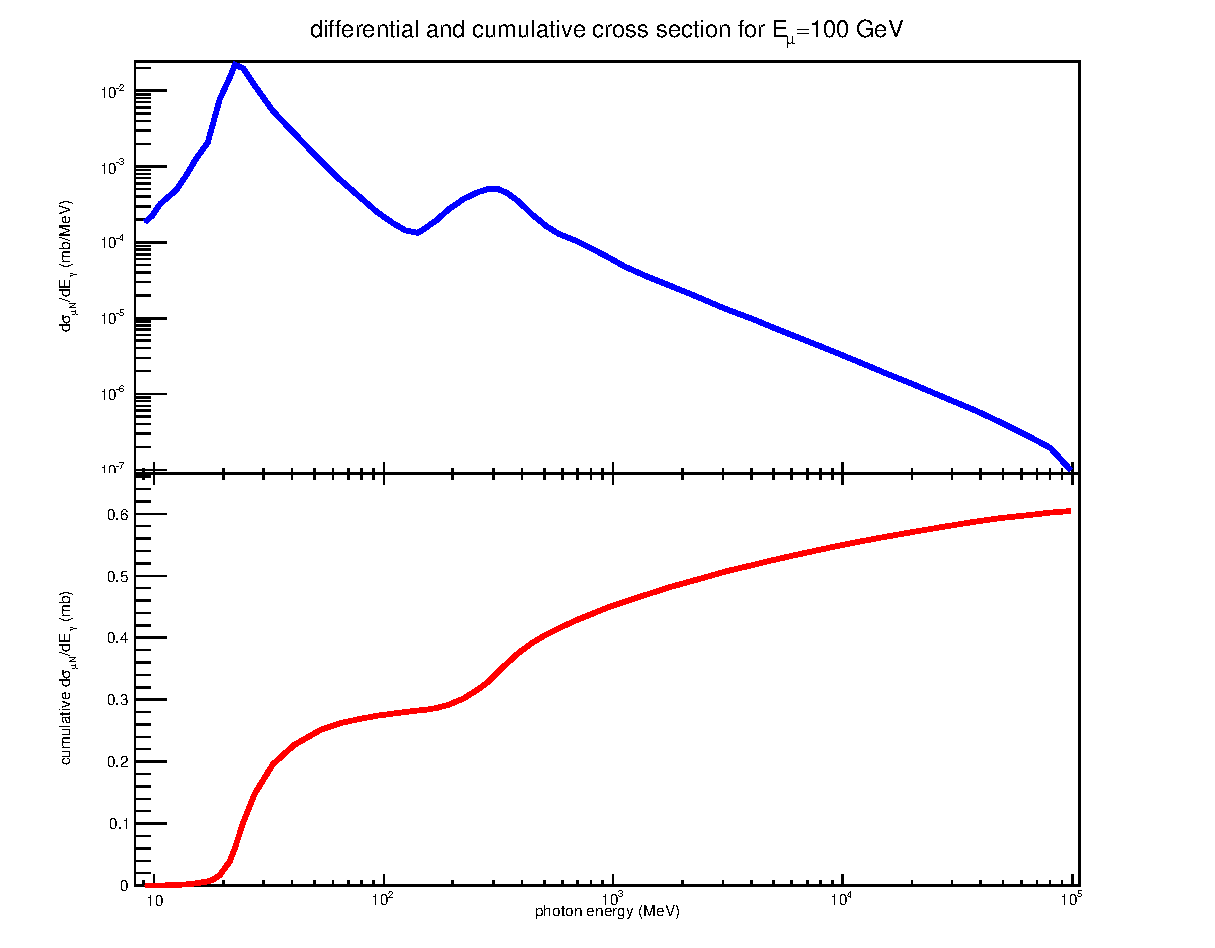
\includegraphics[width=.8\textwidth]{figures/chap6/muN_diff_cumul_cross_section.eps}
	\caption{Top: Muon nucleus differential cross section for 100 GeV muons. Bottom: Cumulative muon nucleus cross section for 100 GeV muons.}
	\label{fig:folded_cross_section}
\end{figure}
The integral of the differential cross section over all photon energy gives the total cross section $\sigma=0.6$ mb. Therefore the neutron yield is
\begin{equation}
	Y_n=\frac{0.6(mb)\times 10^{-27}\left(\frac{cm^2}{mb}\right)\times 6.02\times10^{23}\left(\frac{1}{mol}\right)}{12\left(\frac{g}{mol}\right)}=3\times 10^{-5} (cm^2/g)
\end{equation}
The cumulative cross section shows that the GDR contribution to the total cross section is roughly the same as the contribution from $\Delta$ production and higher energy processes. The yield calculated this way is in rough agreement with the data to be presented in Chapter~\ref{chap:results}. The discrepancy is probably due to higher neutron multiplicity, secondary interactions, and residual high energy interactions.
  \chapter{Neutron Yield Analysis}\label{chap:results}

%\section{Methodology}
%
%Ideally if one wants to measure the neutron yield by muons, one can shoot a monoenergetic muon beam at an infinite-long target and surround the target with a $4\pi$ detector which are able to identify and measure the momentum of all generated particles. This kind of idealization can be achieved closely with Daya Bay experiment.
%
%\begin{figure}
%\centering
%\begin{tikzpicture}
%	\draw (0,0) ellipse (.1cm and .2cm);
%	\draw (0,0) ellipse (1cm and 2cm);
%	\draw (0,.2) -- (3,.2);
%	\draw (0,-.2) -- (3,-.2);
%\end{tikzpicture}
%\caption{An ideal muon induced neutron measurement} \label{fig:IdealMuN}
%\end{figure}
%
%Suppose we know the muon track with some reconstruction algorithm. For those muons passing through the inner acrylic vessel(IAV), we can form a imaginary cylinder coaxial with the track which is fully contained in the IAV. If we fix the radius of the imaginary cylinder, for each track we have to adjust its length so as to make the cylinder fully contained in the IAV. Only neutrons captured in the imaginary cylinder count. If we concatenate the imaginary cylinders one after another, the ideal experiment is approximately realized, with some differences,
%\begin{enumerate}
%	\item Underground muons are not monoenergetic.
%	\item The imaginary cylinders serve as both the target and the detector.
%	\item Generated particles are hard to detect except neutrons.
%\end{enumerate}
%
%Although most underground experiments are not designed for measuring the neutron yield by muons, a in situ measurement of neutron background is still desirable. Since the energy of the underground muons can never be controlled, instead of measuring neutron yield as a function of the incident muon energy, a common practice is to measure neutron yield as a function of the incident \emph{mean} muon energy. And since this measurement is \emph{inclusive}, we don't have to know every detail of each intermediate particle leading to neutron production.

\section{Methodology}
%We propose a track-by-track geometric method to account for the neutron spill-in/spill-out effects which can be compared with a full neutron Monte Carlo simulation once it is available.
We measured the neutron yield on a track-by-track basis by choosing a well-defined fiducial volume for the produced neutrons, and corrected for inefficiencies by simple Monte Carlo simulations.

Neutron yield is the number of neutrons produced by a muon when it traverses a unit length of the material. In this study we are interested in the neutrons produced in the target material, GdLS. The GdLS not only serves as the target, but also serves as the neutron detector. Once a produced neutron is captured on Gd, the neutron position can be reconstructed with a 20 cm resolution~\cite{docdb7334}. In Daya Bay's experimental halls, muons come at all angles and penetrate the inner acrylic vessel (IAV) from all points and angles. Assuming the neutron capture position is axially symmetric around the muon track, a cylindrical fiducial volume can be constructed around the track fully enclosed in the GdLS. We consider the spill-in/spill-out corrections for the longitudinal and lateral directions separately.

\begin{figure}[ht]
	\centering
	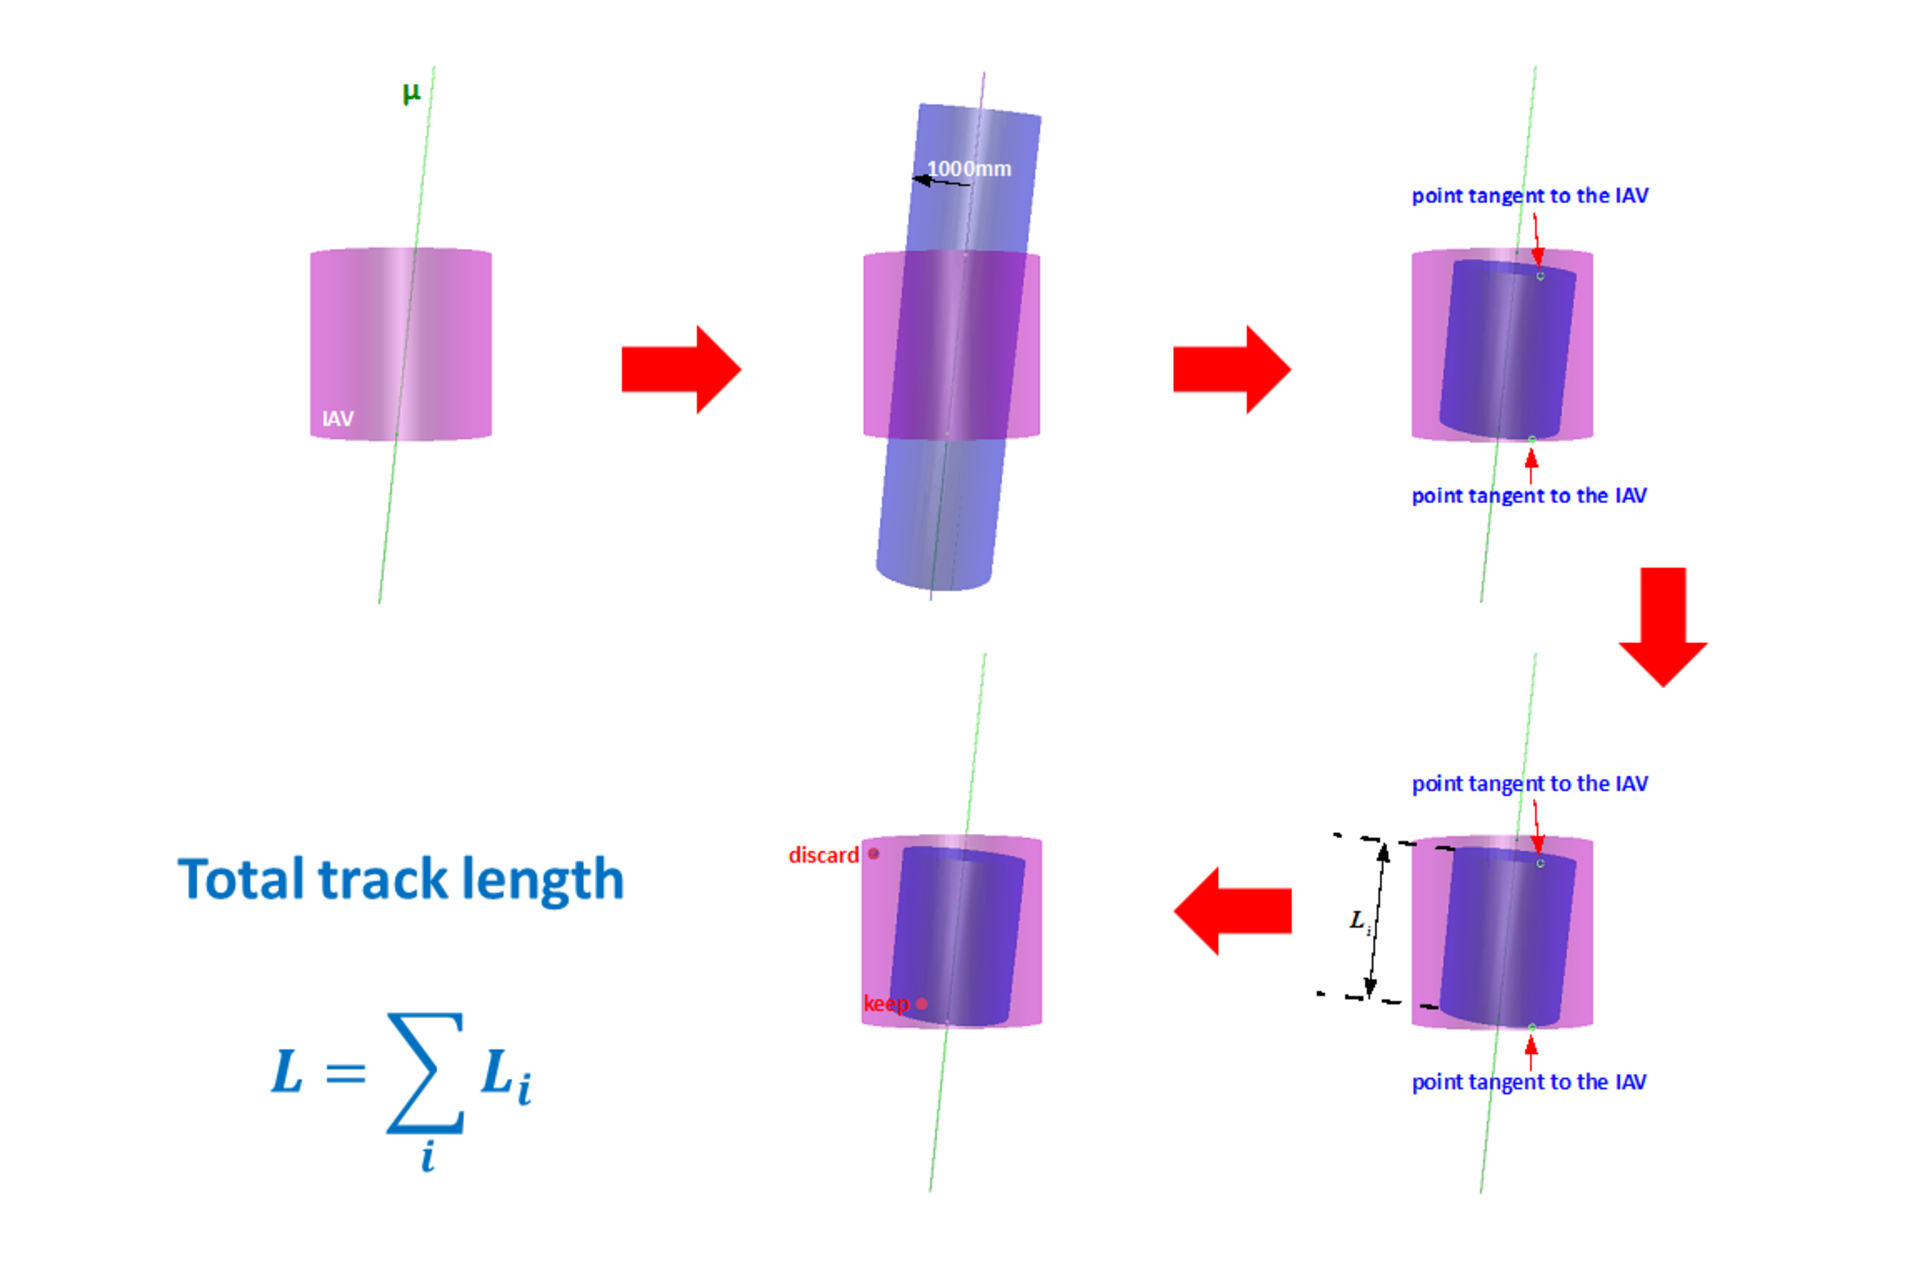
\includegraphics[width=\textwidth]{figures/chap7/fiducial_illustration.eps}
	\caption{A cartoon showing how a symmetric fiducial volume is constructed.}
	\label{fig:fiducial_illustration}
\end{figure}

A longest cylinder of one meter radius is inscribed in the IAV. Figure~\ref{fig:fiducial_illustration} shows how a symmetric fiducial volume can be constructed given a reconstructed muon track. The details of the construction is described in Appendix~\ref{app:a}.
After constructing the fiducial volume, the height of the inscribed fiducial cylinder is taken as the muon track length. Only neutrons captured within the fiducial cylinder are kept.


\section{Event Selection}

\subsection{Muon Selection}

Since a muon can traverse multiple detectors at a time, a muon is actually identified as a group of muon triggers across detectors in data.

The muon selection starts with muon triggers grouped in the directory \scriptsize\path{/Event/Data/Physics/Spallation} \normalsize in production files. The grouping first identifies whether a trigger satisfies the MuonAny criteria. MuonAny is the loosest muon tag which includes all triggers with IWS NHIT $>$ 6 or OWS NHIT $>$ 8 or AD charge $>$ 3000 pe or RPC 3/4 or 4/4 layers being fired (i.e., excluding the RPC random triggers). All MuonAny triggers have to be within 300 ns after the first MuonAny trigger in order to form the so called MuonPrompt triggers which completes the muon grouping process. For more details, see Ref.~\cite{docdb6759} . In order to reconstruct a muon track, a valid OWS reconstructed point with PoolSinple algorithm and a valid RPC reconstructed point with RpcSimple algorithm are required. Note that requiring a valid RPC point will rule out RPC random triggers automatically. Finally, in order to apply the fiducial cut, only tracks around which a fiducial cylinder with radius 1000 mm can fit in the IAV are kept.

\vspace{\baselineskip}
To summarize the muon selection criteria, a muon track has to
\begin{itemize}
  \item satisfy MuonAny criteria:
        \\IWS NHIT $>$ 6 or OWS NHIT $>$ 8 or AD charge $>$ 3000 pe or RPC 3/4 trigger,
  \item all MuonAny triggers within 300 ns since the first MuonAny trigger,
  \item valid points with PoolSinple and RpcSimple so that a track is formed by two point connection, and
  \item tracks around which a cylinder with 1000 mm can fit in the IAV.
\end{itemize}

\subsection{Neutron Selection}\label{sec:n_select}

The neutron has to be Gd captured within the fiducial volume. A Gd captured neutron is identified with its energy and timing. Here we use the IBD neutron energy cut, 6 MeV $< E_n <$ 12 MeV. For the timing cut we first choose the upper bound at 1000 $\mu$s after the muon, which could be fine tuned and optimized. The lower bound is set at 20 $\mu$s after the muon to avoid PMT ringing and AD retriggers. Also the flasher cut is applied to ensure the event is physical.

\vspace{\baselineskip}
To summarize the neutron selection criteria, the neutron has to satisfy the following:
\begin{itemize}
  \item 6 MeV $<$ $E_n$ $<$ 12 MeV,
  \item 20 $\mu$s $<$ $t_n-t_\mu$ $<$ 1000 $\mu$s,
  \item within the fiducial volume constructed in muon selection, and
  \item non-flasher event.
\end{itemize}


\section{Neutron Yield}
Measuring the neutron yield is closely related to measuring the muon-nucleus total interaction cross section since the number of neutrons produced can be written as
\begin{equation} \label{eq:neutron_number}
	\bar{N}_n=n\left\langle\nu\sigma\right\rangle\ell=\frac{\rho N_A}{A}\left\langle\nu\sigma\right\rangle\ell
\end{equation}
where $\bar{N}_n$ is the mean number of neutrons produced per muon, $n$ is the number density of the medium nuclei the muon traverses, $\nu$ is the neutron multiplicity per interaction, $\sigma$ is the inclusive neutron production cross section, $\ell$ is the mean track length of the muon, $\rho$ is the mass density of the medium, $N_A$ is the Avogadro number, and $A$ is the atomic mass of the medium. Because muons could interact with different nuclei in the medium and produce different number of neutrons, the mean value of the product $\left\langle\nu\sigma\right\rangle$ is used.

Experimentally, the neutron yield is given by
\begin{equation} \label{eq:ideal_neutron_yield}
	Y_n=\frac{\bar{N}_n}{\ell\rho}=\frac{N_n}{L\rho}
\end{equation}
where $Y_n$ is the neutron yield, $N_n$ is the total number of neutrons produced by all selected muons and $L$ is the total muon track length traversed by all selected muons.

From Eqs.~\ref{eq:neutron_number} and ~\ref{eq:ideal_neutron_yield} the mean value of the product of the neutron multiplicity and the muon-nucleus total interaction cross section is
\begin{equation}
	\left\langle\nu\sigma\right\rangle=\frac{Y_nA}{N_A}
\end{equation}

However, since 100\% neutron detection efficiency cannot be achieved experimentally due to the neutron selection cuts and finite detector acceptance, the produced number of neutrons is determined by $N_n^s/\epsilon$, the number of observed neutrons corrected by the total detection efficiency which is a product of several efficiency terms. In this study, the total detection efficiency
\begin{equation}
	\epsilon=\epsilon_{Gd}\epsilon_E\epsilon_T\epsilon_{acc}
\end{equation}
where $\epsilon_{Gd}$ is the Gd capture ratio, $\epsilon_E$ is the energy cut efficiency, $\epsilon_T$ is the timing cut efficiency and $\epsilon_{acc}$ is the detector acceptance due to the fiducial volume cut.

The yield formula used in this study is hence
\begin{equation}
	Y_n=\frac{N_n^s}{\epsilon_{Gd}\epsilon_E\epsilon_T\epsilon_{acc}L\rho}
\end{equation}

Since the muon-nucleus total interaction cross section depends on the muon energy, the neutron yield also does. It is standard to parametrize the energy dependence as a power law~\cite{Zatsepin1965},
\begin{equation}
	Y_n(\bar{E}_\mu)=\alpha\bar{E}_\mu^\beta
\end{equation}
where $\bar{E}_\mu$ is the mean muon energy and $\alpha$ and $\beta$ are parameters to be fitted with data. This formula is largely confirmed by FLUKA and GEANT4 simulations~\cite{Wang2001}~\cite{Araujo2005}~\cite{Mei2006}~\cite{Malgin2008} as well as by measurements~\cite{Bezrukov1973}~\cite{Enikeev1987}~\cite{Aglietta1989}. However large tensions in the values of $\alpha$ and $\beta$ still remain. The Daya Bay experiment has three experimental halls each with different overburden. Therefore, Daya Bay, a single experiment, can measure three yield values corresponding to three different mean muon energies.

There are therefore 8 terms to be determined in order to measure the yield as a function of the mean muon energy, namely $N_n^s$, $\epsilon_{Gd}$, $\epsilon_E$, $\epsilon_T$, $\epsilon_{acc}$, $L$, $\rho$, and $\bar{E}_\mu$. In the following sections each term and its uncertainty will be discussed in detail.

The discussion will start with more widely studied quantities and move on to the quantities more specific to this study.

\subsection{Target Density \texorpdfstring{$\rho$}{rho}}
The GdLS density is~\cite{docdb6615}
\begin{equation}
	\rho=0.861\pm 0.001\text{ }g/cm^3
\end{equation}

\subsection{Gd Capture Ratio \texorpdfstring{$\epsilon_{Gd}$}{epsilon Gd}}
Spallation neutrons generated in the target mass, GdLS, may not all be captured on Gd. Some could be captured on H or other nuclei. Some are not captured at all and leave the detector, which we call spill-out neutrons. There are also spill-in neutrons, namely neutrons generated outside and transported into the fiducial volume and get captured on Gd. Since in this study we select only the Gd captured neutrons, we have to determine this efficiency which is often called the Gd capture ratio.

Many studies had been done on the Gd capture ratio with spallation neutrons~\cite{docdb7273}~\cite{docdb7524}~\cite{docdb7525}, calibration sources~\cite{docdb7273}~\cite{docdb7525}, special calibration runs~\cite{docdb8280}~\cite{docdb8473}~\cite{docdb8501}~\cite{docdb9226}~\cite{docdb9273}, and Monte Carlo simulation~\cite{docdb7730}. However, different studies adopt slightly different definitions of this ratio. Here we define the Gd capture ratio as
\begin{equation} \label{eq:gd_capture_ratio}
	\epsilon_{Gd}=\frac{\text{number of neutrons generated in GdLS and captured on Gd}}{\text{number of neutrons generated in GdLS}}
\end{equation}

We use the more up-to-date study~\cite{docdb9273}. In this study a complete comparison between AmC, AmBe, PuC, and Monte Carlo is given and the efficiency due to energy cuts is corrected for resulting in a $\epsilon_{Gd}$ definition which coincides with Eq.~\ref{eq:gd_capture_ratio}. The final result is quoted as,
\begin{equation}
  \epsilon_{Gd}=85.2\%\pm 0.4\%
\end{equation}


\subsection{Energy Cut Efficiency \texorpdfstring{$\epsilon_{E}$}{epsilon E}}

One of the signatures of a neutron captured on Gd is the 8 MeV $\gamma$ energy released from the de-excitation of Gd*. Therefore, we use the 8 MeV energy cut efficiency published in the IBD analysis~\cite{dayabay2012_1}, combining the correlated and uncorrelated uncertainties,
\begin{equation}
	\epsilon_{E}=90.9\%\pm 0.61\%
\end{equation}


\subsection{Capture Time Cut Efficiency \texorpdfstring{$\epsilon_{T}$}{epsilon T}}

The other signature of a neutron captured on Gd is the capture time whose mean value is $\sim 28\mu s$. Figure~\ref{fig:IBD_capture_time} shows the IBD neutron capture time distribution. The distribution is not a simple exponential but has a rising edge in the beginning of the spectrum. A 2-exponential fit to model the whole spectrum~\cite{docdb7299}, one of which accounts for the rising edge due to the thermalization of neutrons.
\begin{figure}
	\centering
	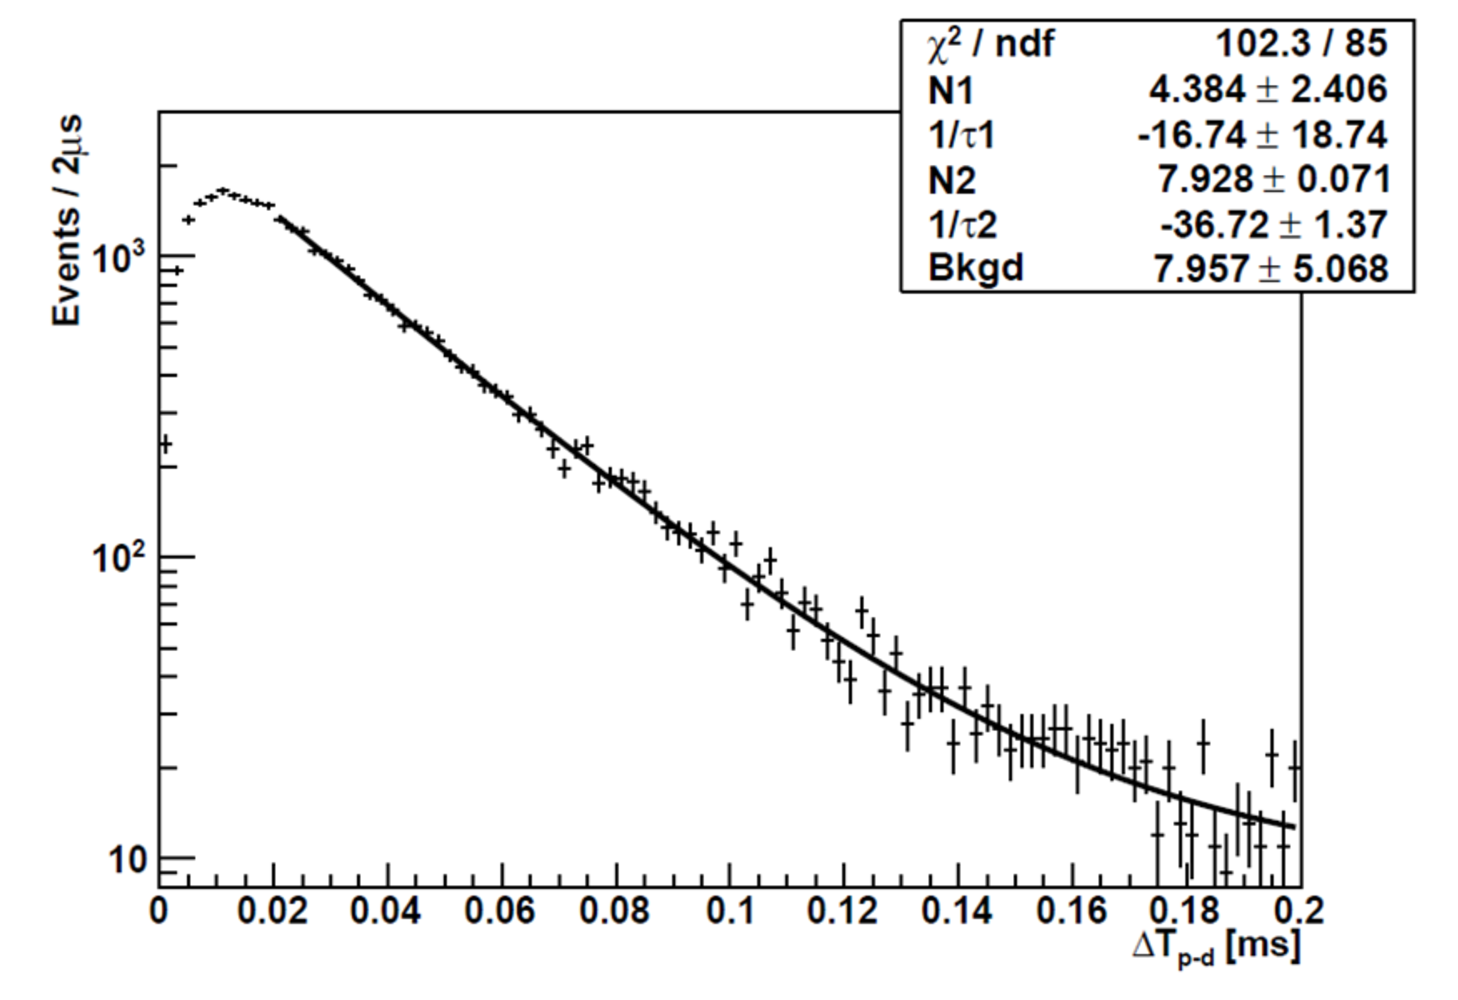
\includegraphics[width=.6\textwidth]{figures/chap7/IBD_capture_time.eps}
	\caption[IBD neutron capture time distribution]{IBD neutron capture time distribution~\cite{docdb7299}}
	\label{fig:IBD_capture_time}
\end{figure}

In the spallation neutron case, there are several differences. First, the initial energy of the spallation neutrons can be higher than the IBD neutrons, leading to a longer thermalization time. Second, after the muon passes through the AD, the huge amount of energy distorts the PMT signal for about 10 $\mu$s and produce retrigger events. Figure~\ref{fig:spallation_capture_time} shows the capture time distribution of EH1 AD1.
\begin{figure}[ht]
	\centering
	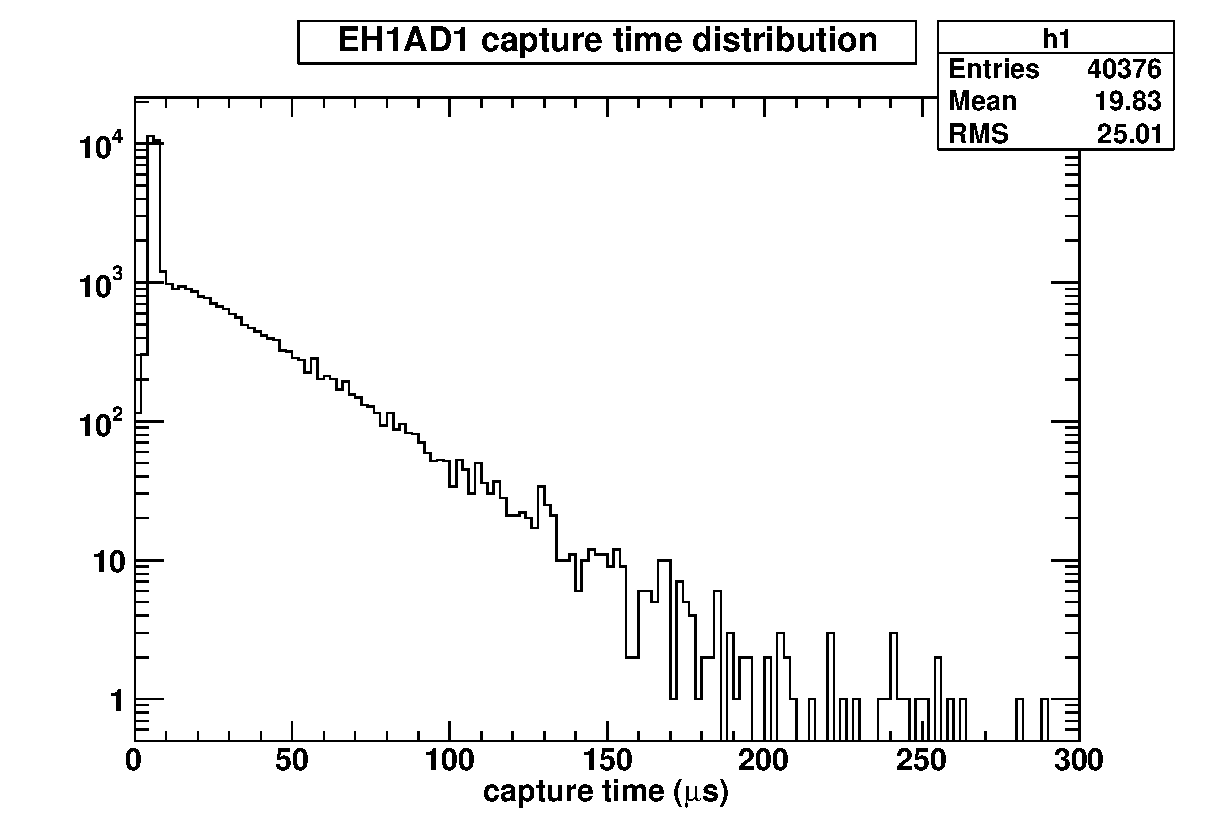
\includegraphics[width=.6\textwidth]{figures/chap7/spallation_neutron_capture_time.eps}
	\caption{Spallation neutron capture time distribution}
	\label{fig:spallation_capture_time}
\end{figure}
Clearly there is a retrigger peak between 4 and 10 $\mu$s. In the 2-exponential function model, we can do a linear interpolation between the time with the left and right bins. Then we fit the distribution to a 2-exponential function, and use the fitted function to estimate the capture time cut efficiency. Figure~\ref{fig:fit_capture_time} shows the fit result of EH1 AD1.
\begin{figure}[ht]
	\centering
	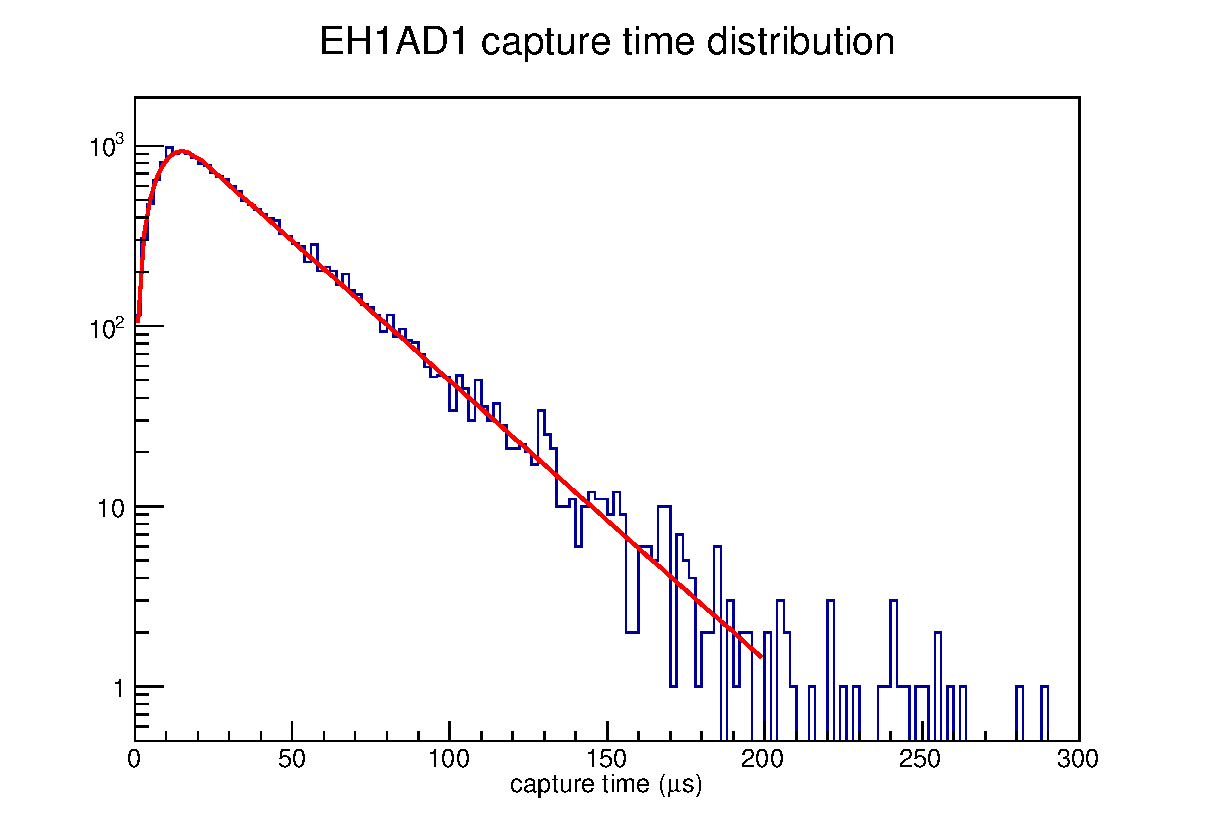
\includegraphics[width=.6\textwidth]{figures/chap7/fit_capture_time.eps}
	\caption{2-exponential fit to the interpolated capture time distribution}
	\label{fig:fit_capture_time}
\end{figure}
The efficiency is then obtained by the formula
\begin{equation}
	\epsilon_T=\frac{\int_{20}^{\infty}f(t)dt}{\int_{0}^{\infty}f(t)dt}
\end{equation}
The systematic uncertainty of this number is obtained by varying the counts in the 4 to 10 $\mu$s window, fitting the distribution with the 2-exponential function, and calculating the efficiency with the new fitted function. A $5\%$ relative uncertainty is found for all ADs. The results of capture time cut efficiency are summarized in Table~\ref{tab:timing_efficiency}.
\begin{table}[ht]
	\centering
	\begin{tabular}{|c|c|}
		\hline
		detector & $\epsilon_T$ (\%) \\
		\hline
		EH1 AD1 & 0.64$\pm$0.03 \\
		\hline
		EH1 AD2 & 0.64$\pm$0.03 \\
		\hline
		EH2 AD1 & 0.63$\pm$0.03 \\
		\hline
		EH3 AD1 & 0.66$\pm$0.03 \\
		\hline
		EH3 AD2 & 0.66$\pm$0.03 \\
		\hline
		EH3 AD3 & 0.67$\pm$0.03 \\
		\hline
	\end{tabular}
	\caption{Capture time cut efficiency for each AD.}
	\label{tab:timing_efficiency}
\end{table}


\subsection{Number of Selected Neutrons \texorpdfstring{$N_n^s$}{N} and Total Track Length \texorpdfstring{$L$}{L}}
There are uncertainties in the vertex in the RPC and OWS reconstruction. Thus, the RPC-OWS connection is also subject to these uncertainties and deviates from the true track, which in turn leads to a different fiducial cylinder from the real one. Not only the total track length, which is the sum of the heights of all fiducial cylinders, but also the number of neutrons included in the fiducial volume will change. So we discuss the number of selected neutrons together with the total track length, and estimate the uncertainties with a toy Monte Carlo which takes into account the geometry effects concerning the two numbers at the same time.

Neutron selection criteria were stated in Section~\ref{sec:n_select}. A side band time window between [1020, 2000] $\mu$s is used for the background spectrum. Figure~\ref{fig:energy_spectrum} shows the results for each AD.
\begin{figure}[ht]
	\centering
	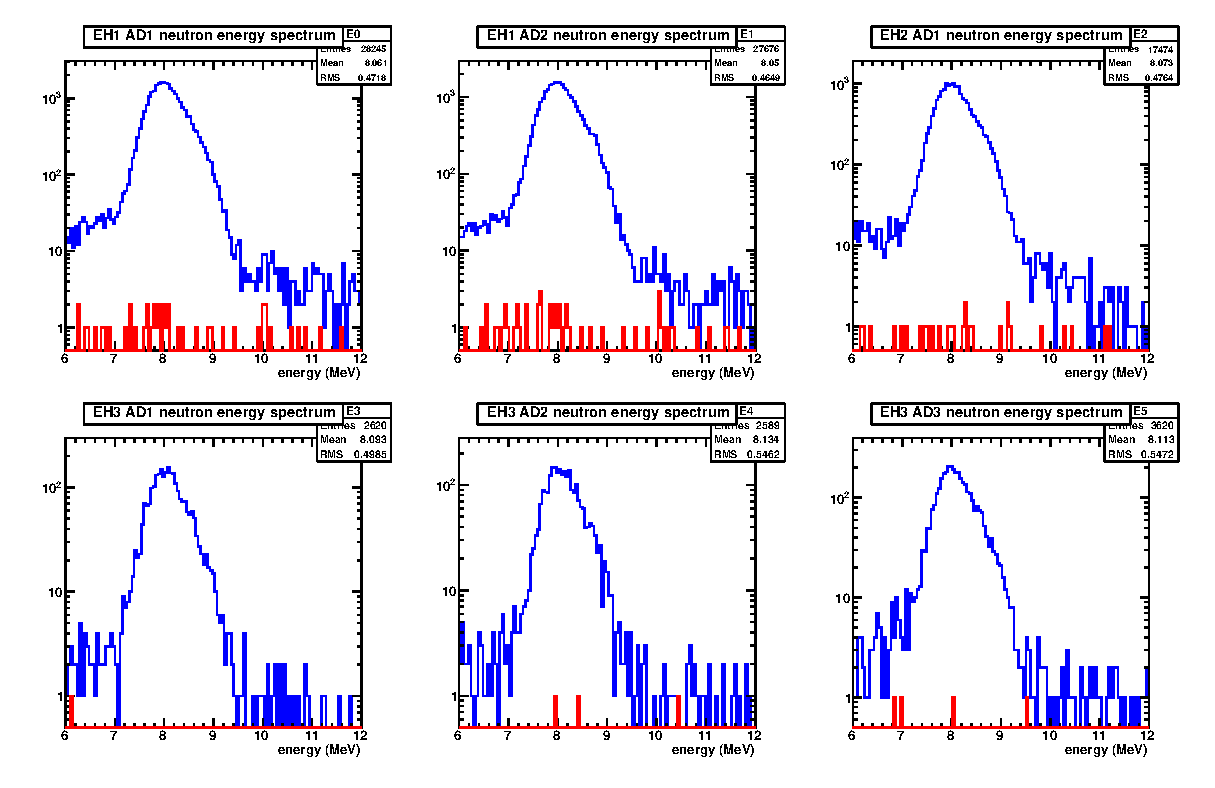
\includegraphics[width=\textwidth]{figures/chap7/neutron_energy_spectrum.eps}
	\caption{Neutron and background energy spectrum.}
	\label{fig:energy_spectrum}
\end{figure}
The number of selected neutron is $N_n^s=N_{sig}-N_{bkg}$, where $N_{sig}$ and $N_{bkg}$ are the numbers of events in the signal and the background windows, respectively. The statistical uncertainty is computed according to $\sqrt{N_{sig}+N_{bkg}}$. Table~\ref{tab:number_of_neutrons} lists the results for $N_{sig}$ and $N_{bkg}$.
\begin{table}[ht]
	\centering
	\begin{tabular}{|c|c|c|}
		\hline
		detector & $N_{sig}$ & $N_{bkg}$ \\
		\hline
		EH1 AD1 & 28245 & 44 \\
		\hline
		EH1 AD2 & 27676 & 51 \\
		\hline
		EH2 AD1 & 17474 & 28 \\
		\hline
		EH3 AD1 & 2620 & 1 \\
		\hline
		EH3 AD2 & 2589 & 3 \\
		\hline
		EH3 AD3 & 3620 & 4 \\
		\hline
	\end{tabular}
	\caption{Results of events in the signal and the background windows.}
	\label{tab:number_of_neutrons}
\end{table}

The total track length is obtained by summing the lengths of the fiducial cylinders. The results are listed in Table~\ref{tab:total_track_length}.
\begin{table}[ht]
	\centering
	\begin{tabular}{|c|c|}
		\hline
		detector & total track length (cm) \\
		\hline
		EH1 AD1 & $1.17\times 10^9$ \\
		\hline
		EH1 AD2 & $1.13\times 10^9$ \\
		\hline
		EH2 AD1 & $6.90\times 10^8$ \\
		\hline
		EH3 AD1 & $7.78\times 10^7$ \\
		\hline
		EH3 AD2 & $7.26\times 10^7$ \\
		\hline
		EH3 AD3 & $9.69\times 10^7$ \\
		\hline
	\end{tabular}
	\caption{Total track length for each AD.}
	\label{tab:total_track_length}
\end{table}

The systematic uncertainties for $N_n^s$ and $L$ are estimated by a toy Monte Carlo which takes into account the uncertainties due to the vertex reconstructions. A deviation in track will change the construction of the fiducial cylinder, which might in turn change the inclusion or exclusion of a neutron. Therefore this toy Monte Carlo will estimate the two systematic uncertainties at the same time. The procedure of the toy Monte Carlo is:
\begin{itemize}
	\item Take the small muon Monte Carlo sample.
	\item Without loss of generality, take the RPC and OWS reconstructed vertices as true vertices.
	\item Generate a true neutron vertex according to a uniform distribution along the track direction and a lateral distance according to the 2D gaussian function $re^{-\frac{r^2}{2\sigma^2}}$ where $\sigma=$ 40 cm. From data we know when $r$ is small this is a good approximation and 40 cm is obtained from data. The vertex could be anywhere in the IAV in order to study the inclusion/exclusion of neutrons due to the uncertainties in RPC, OWS and neutron vertices.
	\item Randomly select a point within the 25 cm $\times$ 25 cm square due to RPC resolution.
	\item Randomly generate a point around the OWS vertex with a random direction and a radial distance following the 3D gaussian function $r^2e^{-\frac{r^2}{2\sigma^2}}$, where $\sigma=$ 50 cm.
	\item Randomly generate a point around the neutron vertex with a random direction and a radial distance following the 3D gaussian function $r^2e^{-\frac{r^2}{2\sigma^2}}$, where $\sigma=$ 20 cm by Yasu's AdSimple resolution.
	\item Form the ``smeared'' track and construct the fiducial volume.
	\item For each neutron, record its selection status before and after the smearing process.
	\item For the true and smeared case, sum up the fiducial cylinder lengths and the number of neutrons in the fiducial cylinder.
\end{itemize}
The results show a $1\%$ uncertainty in the total track length and a $10\%$ uncertainty in the number of selected neutrons. Since the total uncertainty is dominated by the neutron selection uncertainty, the full covariance matrix is not calculated\footnote{
For a two variable differentiable function $f(a,b)$ the uncertainty in $f$ is
\begin{equation}
	\left(\frac{\sigma_f}{f}\right)^2\approx\left(\frac{\sigma_a}{a}\right)^2+\left(\frac{\sigma_b}{b}\right)^2+2\left(\frac{\sigma_a}{a}\right)\left(\frac{\sigma_b}{b}\right)\rho_{ab}
\end{equation}
where $\sigma_f$, $\sigma_a$, and $\sigma_b$ are uncertainties in $f$, $a$, and $b$, respectively, and $\rho_{ab}$ is the correlation coefficient of $a$ and $b$. Since $-1 \leq \rho_{ab} \leq 1$, if $\frac{\sigma_a}{a}\gg\frac{\sigma_b}{b}$, $\frac{\sigma_f}{f}\approx\frac{\sigma_a}{a}$.
}.


\subsection{Lateral Acceptance \texorpdfstring{$\epsilon_{acc}$}{epsilon}}
The neutrons are expected to be boosted forward. There is space before the fiducial cylinder. If neutrons are produced upstream, they enter the cylinder even if they are not produced inside. As a result, the neutron flux entering the fiducial cylinder from upstream of the track equals the neutron flux leaving the fiducial cylinder. We only need the lateral distribution to determine the detector acceptance. Figure~\ref{fig:z_distribution} shows the distribution of the relative longitudinal position of the capture point relative to the cylinder center. It clearly shows a uniform distribution, which shows spill-in equals spill-out in the longitudinal direction.
\begin{figure}[ht]
	\centering
	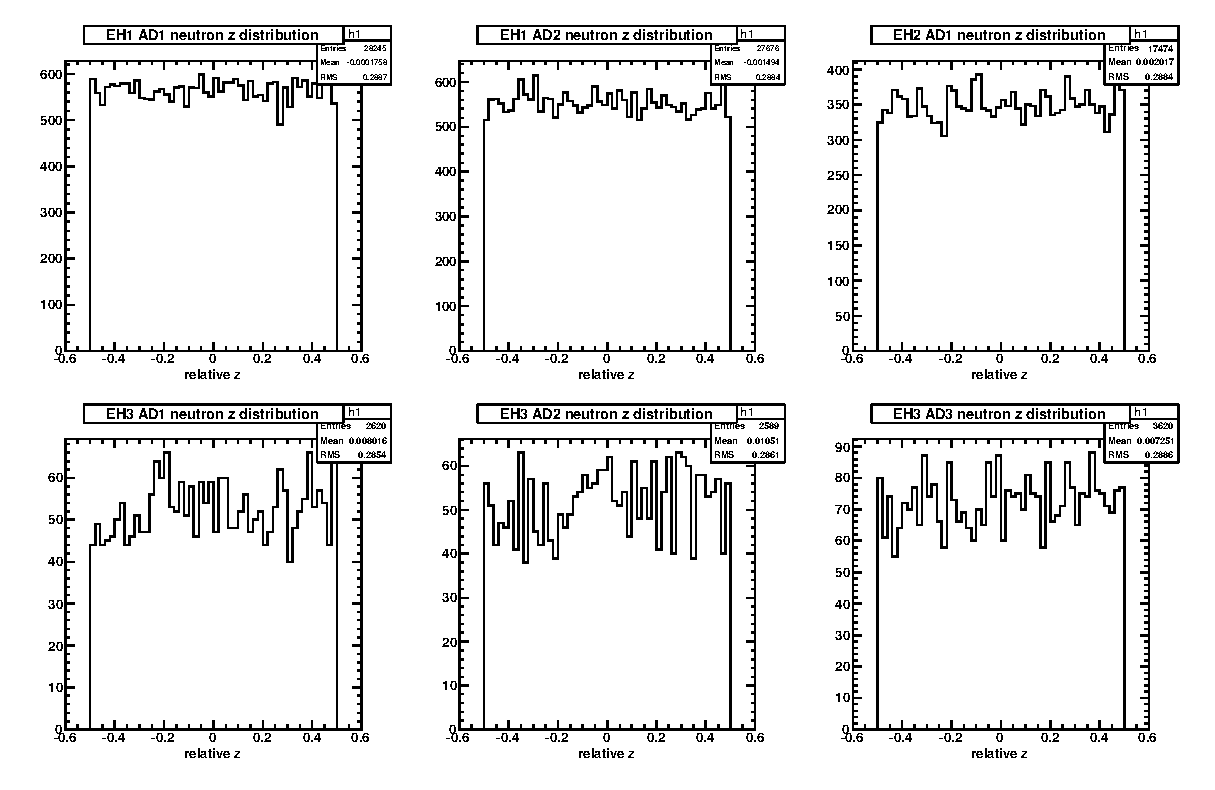
\includegraphics[width=\textwidth]{figures/chap7/z_distribution.eps}
	\caption{Relative longitudinal capture position with respect to the fiducial cylinder center.}
	\label{fig:z_distribution}
\end{figure}

To estimate the lateral acceptance due to the finite volume of the fiducial cylinders, we lift the muon selection criteria that a fiducial cylinder is able to be constructed. This mean we practically use every muons which have a track reconstructible by RPC-OWS connection. After the track reconstruction, we search for Gd captured neutrons and register the lateral distances to the track. Figure~\ref{fig:lateral_distance_no_cylinder} shows the lateral distance distribution for each AD.
\begin{figure}[ht]
	\centering
	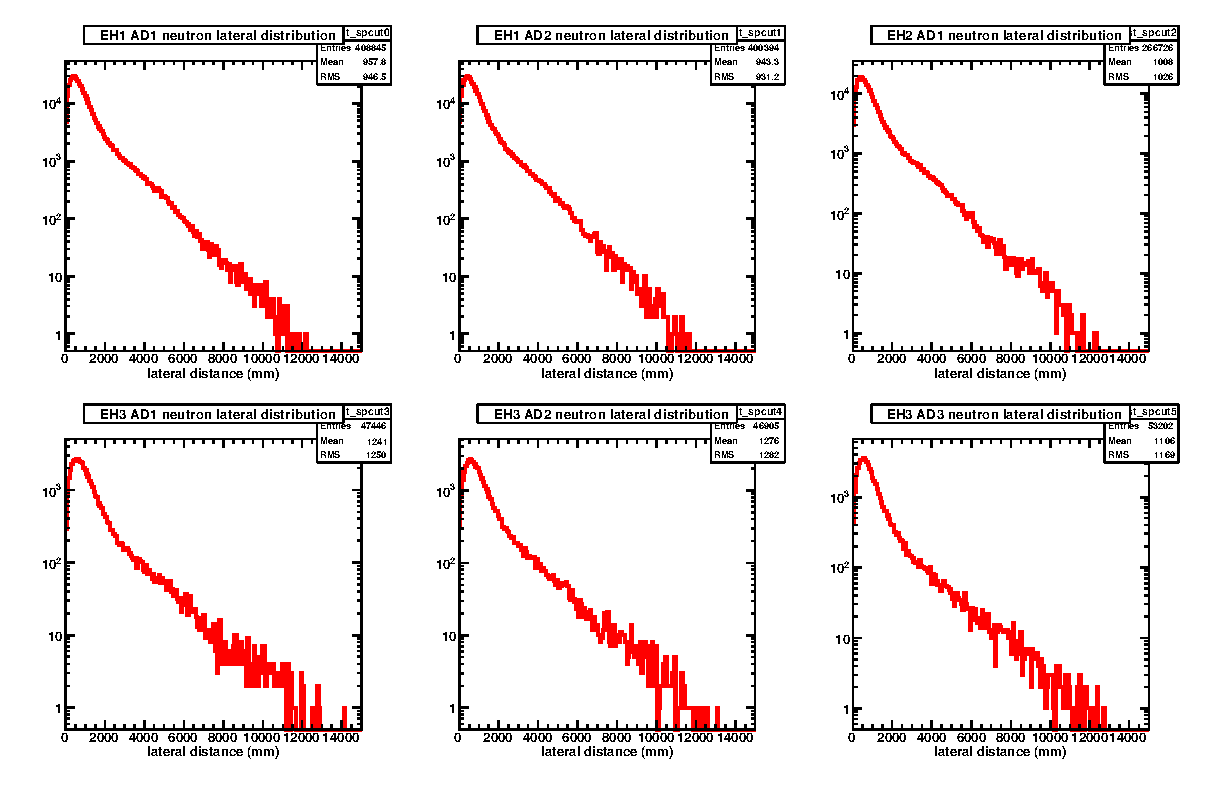
\includegraphics[width=\textwidth]{figures/chap7/lateral_distance_no_cylinder.eps}
	\caption{Neutron lateral distribution for muons with a valid RPC-OWS track.}
	\label{fig:lateral_distance_no_cylinder}
\end{figure}
Table~\ref{tab:lateral_acceptance} shows the lateral acceptance estimated by the fraction of the number of events with lateral distances smaller than 1000 mm.
\begin{table}
	\centering
	\begin{tabular}{|c|c|}
		\hline
		detector & lateral acceptance ($\%$) \\
		\hline
		EH1 AD1 & $0.60\pm 0.06$ \\
		\hline
		EH1 AD2 & $0.60\pm 0.06$ \\
		\hline
		EH2 AD1 & $0.61\pm 0.06$ \\
		\hline
		EH3 AD1 & $0.57\pm 0.06$ \\
		\hline
		EH3 AD2 & $0.56\pm 0.06$ \\
		\hline
		EH3 AD3 & $0.64\pm 0.06$ \\
		\hline
	\end{tabular}
	\caption{Lateral acceptance estimated by the method described in the text.}
	\label{tab:lateral_acceptance}
\end{table}


\subsection{Mean Muon Energy \texorpdfstring{$\bar{E}_\mu$}{E}}
Daya Bay cannot measure muon energy; Daya Bay only measures muon \emph{deposited} energy. Therefore, the mean muon energy is obtained by Monte Carlo simulation. A sample of muons for each hall was generated by the MUSIC package which has been incorporated in NuWa. Each MUSIC sample file contains a million muons with energies, angles (polar and azimuthal) on the sea level and energies and angles in the hall after propagation through the rocks. Therefore, for each hall a simulated mean muon energy can be obtained by simply taking the arithmetic mean of the muon energies after propagation. Figure~\ref{fig:muon_energy_spectrum} shows the simulated muon energy spectra \emph{in} the three halls. From these spectra we see that the more overburden a hall has, the harder (i.e., higher energy) the muon energy spectrum is. The mean muon energy for each hall is listed in Table~\ref{table:mean_muon_energy}.
\begin{figure}
	\centering
	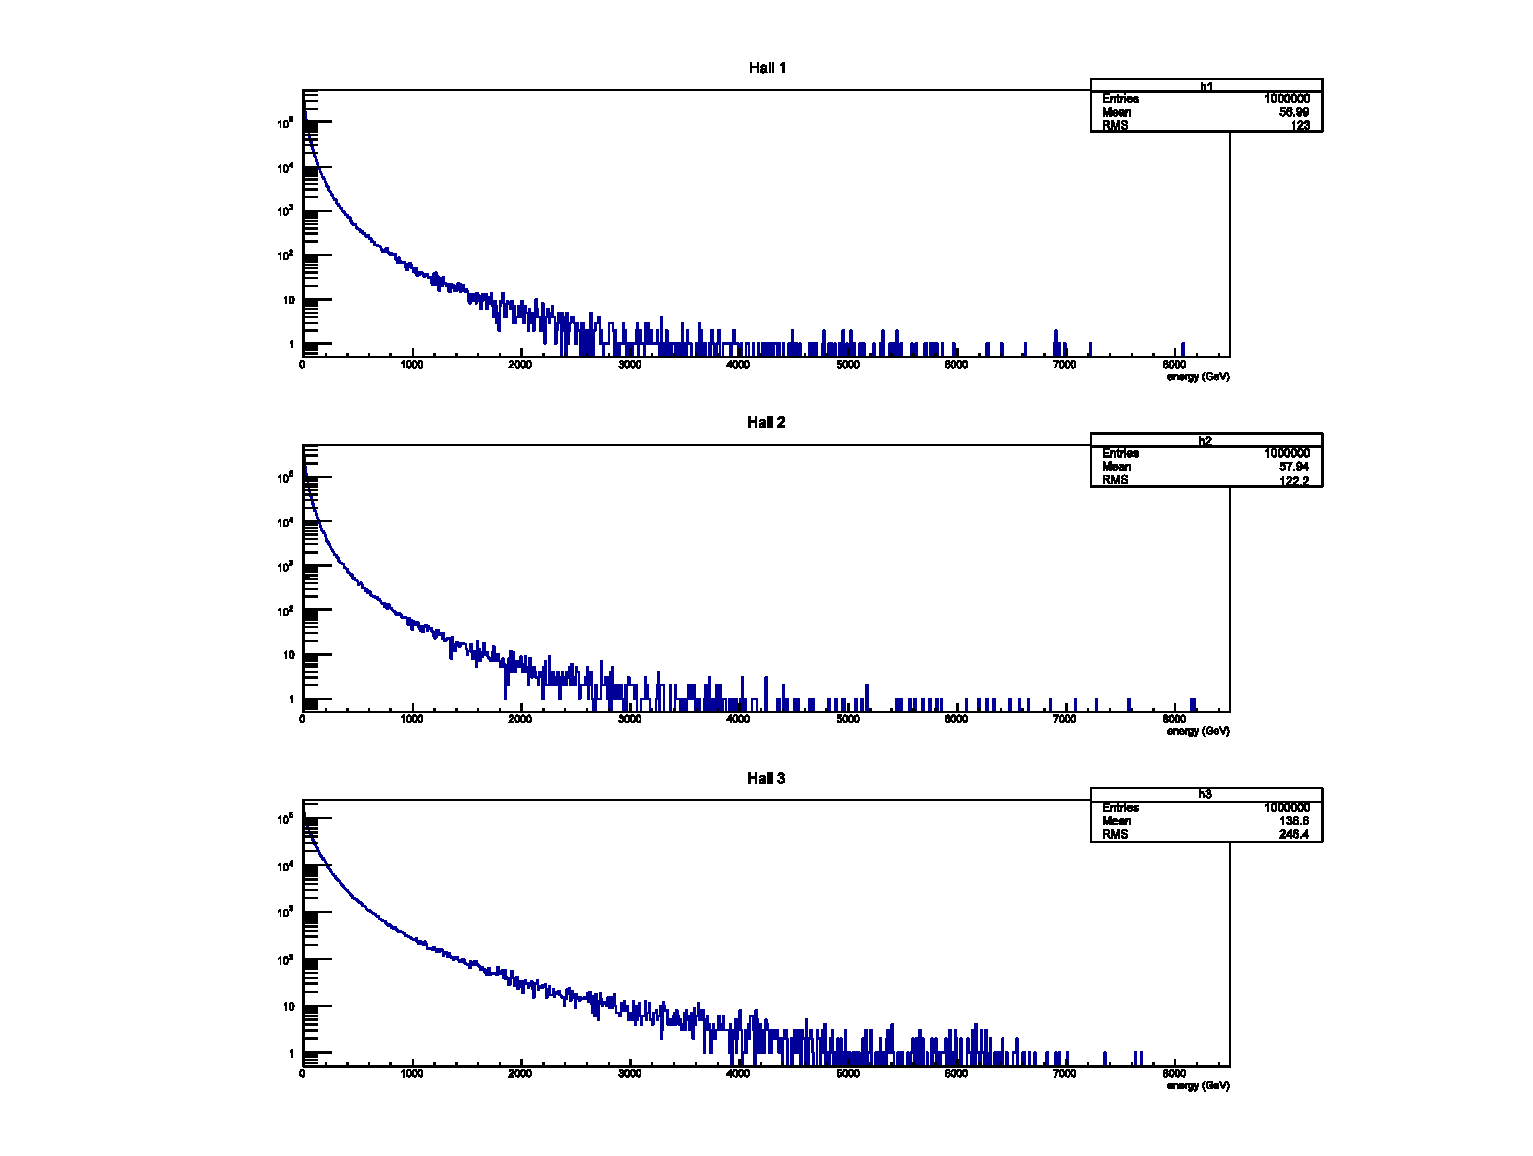
\includegraphics[width=\textwidth]{figures/chap7/muon_energy_spectrum.eps}
	\caption{Simulated muon energy spectra in the three halls.}
	\label{fig:muon_energy_spectrum}
\end{figure}
\begin{table}
	\centering
	\begin{tabular}{cccc}
	\toprule
	& EH1 & EH2 & EH3 \\
	\midrule
	mean muon energy (GeV) & 57 & 58 & 137 \\
	\bottomrule
	\end{tabular}
	\caption{The mean muon energy for each hall by simulation.}
	\label{table:mean_muon_energy}
\end{table}

However, in this study, not all muons are selected. Recall that in the muon selection criteria, a RPC-OWS track has to be formed, which implies a RPC hit. Consequently for an AD, it doesn't see all muons coming from all angles. Instead, it sees muons which happen to go through the RPC, in effect excluding muons with very large polar angles. This "RPC coverage" effect varies from AD to AD. Figure~\ref{fig:rpc_coverage} shows the RPC coverage for each AD in the 3 halls. Take hall 1 as an example. AD1 has more RPC coverage in south east. Therefore AD1 will sample more large angle muons from south east. On the contrary, AD2 samples more large angle muons from north west. Since the mountain overburden is not uniform (see Figure~\ref{fig:muontain_profile}), and since muons incident from different direction go through different amount of rocks, the mean muon energy will not only be different from the hall average, but will have an AD-to-AD variation.
\begin{figure}
	\centering
	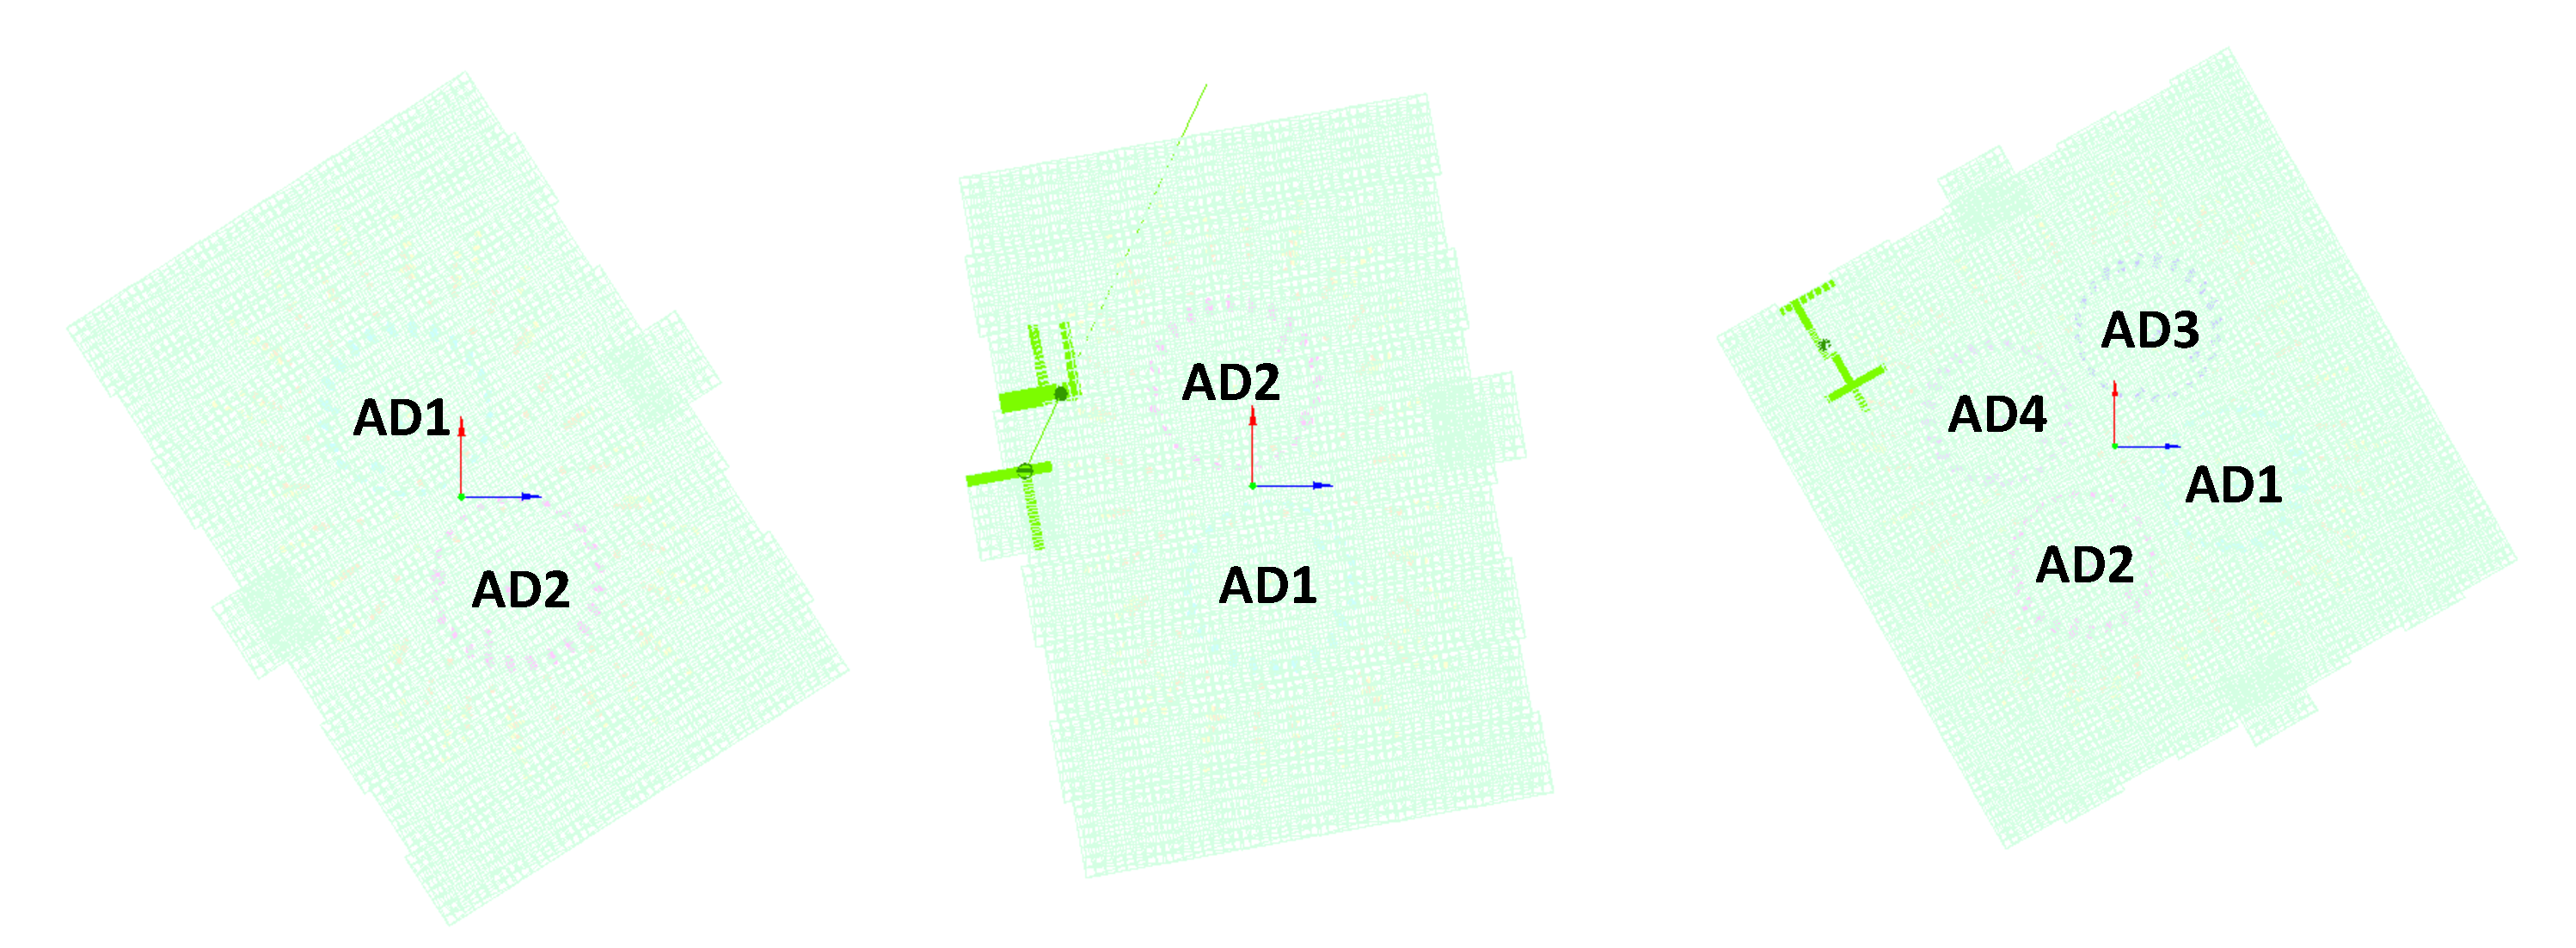
\includegraphics[width=\textwidth]{figures/chap7/RPC_coverage.eps}
	\caption{RPC coverage for each AD in different halls.}
	\label{fig:rpc_coverage}
\end{figure}
\begin{figure}
	\centering
	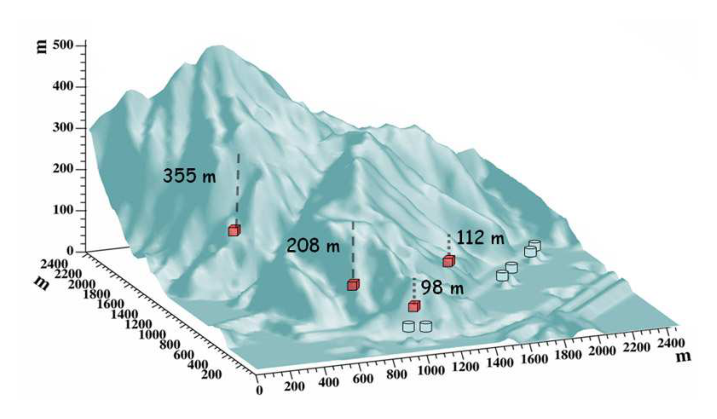
\includegraphics[width=0.7\textwidth]{figures/chap7/mountain_profile.eps}
	\caption[Three dimensional profile of Pai Ya Mountain, where the Daya Bay experimental halls are located including the water hall.]{Three dimensional profile of Pai Ya Mountain, where the Daya Bay experimental halls are located including the water hall.~\cite{dayabay_proposal}}
	\label{fig:muontain_profile}
\end{figure}

To account for the RPC coverage effect, a resampling of the MUSIC sample was done. The procedure of the resampling is:
\begin{itemize}
	\item In the RPC plane, generate a random point.
	\item Generate a direction according to the angular distribution in the MUSIC sample.
	\item Form the track. If for the track a fidicial cylinder can be constructed for a particular AD, keep it. Otherwise don't keep it.
	\item Repeat the procedure for all ADs.
\end{itemize}
The results of the resampling is shown in Table~\ref{tab:mean_muon_energy}. A $5\%$ systematic uncertainty due to the incomplete knowledge in the rock composition and the resolution in the mountain profile is assigned.
\begin{table}
	\centering
	\begin{tabular}{|c|c|}
		\hline
		detector & mean muon energy (GeV) \\
		\hline
		EH1 AD1 & $47\pm 2$ \\
		\hline
		EH1 AD2 & $47\pm 2$ \\
		\hline
		EH2 AD1 & $50\pm 2$ \\
		\hline
		EH3 AD1 & $123\pm 6$ \\
		\hline
		EH3 AD2 & $130\pm 7$ \\
		\hline
		EH3 AD3 & $127\pm 6$ \\
		\hline
	\end{tabular}
	\caption{Mean muon energy seen by each AD.}
	\label{tab:mean_muon_energy}
\end{table}
ADs in the far hall see larger mean muon energies than those in the near halls. This is consistent with the MUSIC simulation (see Table~\ref{table:mean_muon_energy}). The lower mean muon energy seen by the ADs compared with that in the hall from simulation is due to the finite coverage of the RPCs: Requiring the muons to have RPC hits excludes muons with very large zenith angles, which have to go through more rocks and have a harder energy spectrum.


\subsection{Results}
Applying the error propagation formula to the terms, assuming the terms $N_n^s/L$, $\epsilon_E$, $\epsilon_{T}$, $\epsilon_{Gd}$, $\epsilon_{acc}$, $\rho$ are independent, the total systematic uncertainty can be combined in quadrature
\begin{equation}
	\left(\frac{\sigma^{syst}_{Y_n}}{Y_n}\right)^2=\left(\frac{\sigma_{N_n^s/L}^{syst}}{N_n^s/L}\right)^2+\left(\frac{\sigma_{\epsilon_E}}{\epsilon_E}\right)^2+\left(\frac{\sigma_{\epsilon_{T}}}{\epsilon_{T}}\right)^2+\left(\frac{\sigma_{\epsilon_{Gd}}}{\epsilon_{Gd}}\right)^2+\left(\frac{\sigma_{\epsilon_{acc}}}{\epsilon_{acc}}\right)^2+\left(\frac{\sigma_{\rho}}{\rho}\right)^2
\end{equation}
Also, the $N_n^s$ contains the statistical uncertainty
\begin{equation}
	\left(\frac{\sigma^{stat}_{Y_n}}{Y_n}\right)^2=\left(\frac{\sigma_{N_n^s}}{N_n^s}\right)^2
\end{equation}
The relative systematic and statistical uncertainties are summarized in Tables~\ref{tab:systematic_uncertainties} and~\ref{tab:statistical_uncertainties}.
\begin{table}[ht]
	\centering
	\begin{tabular}{|c|c|c|c|c|c|c|}
		\hline
		term & $N_n^s/L$ & $\epsilon_E$ & $\epsilon_{T}$ & $\epsilon_{Gd}$ & $\epsilon_{acc}$ & $\rho$ \\
		\hline
		value ($\%$) & $10$ & $0.7$ & $5$ & $0.5$ & $10$ & $0.1$ \\
		\hline
	\end{tabular}
	\caption{Relative systematic uncertainties for terms in the yield formula.}
	\label{tab:systematic_uncertainties}
\end{table}
\begin{table}[ht]
	\centering
	\begin{tabular}{|c|c|c|c|c|c|c|}
		\hline
		detector & EH1 AD1 & EH1 AD2 & EH2 AD1 & EH3 AD1 & EH3 AD2 & EH3 AD3 \\
		\hline
		value ($\%$) & $0.6$ & $0.6$ & $0.8$ & $2$ & $2$ & $2$ \\
		\hline
	\end{tabular}
	\caption{Relative statistical uncertainties for each AD.}
	\label{tab:statistical_uncertainties}
\end{table}
The total uncertainty is again, obtained by quadrature
\begin{equation}
	\left(\frac{\sigma_{Y_n}}{Y_n}\right)^2=\left(\frac{\sigma^{stat}_{Y_n}}{Y_n}\right)^2+\left(\frac{\sigma^{syst}_{Y_n}}{Y_n}\right)^2
\end{equation}
The estimates and uncertainties of the neutron yield for each AD from the estimates of each terms in the yield formula are summarized in Table~\ref{tab:yield}.
\begin{table}
	\centering
	\begin{tabular}{|c|c|c|}
		\hline
		detector & yield ($\times 10^{-5} cm^2/g$) & relative uncertainty ($\%$) \\
		\hline
		EH1 AD1 & $9.72$ & $15$ \\
		\hline
		EH1 AD2 & $9.86$ & $15$ \\
		\hline
		EH2 AD1 & $10.2$ & $15$ \\
		\hline
		EH3 AD1 & $13.9$ & $15$ \\
		\hline
		EH3 AD2 & $14.9$ & $15$ \\
		\hline
		EH3 AD3 & $13.5$ & $15$ \\
		\hline
	\end{tabular}
	\caption{Neutron yields and relative uncertainties for each AD.}
	\label{tab:yield}
\end{table}
The neutron yield as a function of the mean muon energy obtained in this study is plotted in Figure~\ref{fig:yield_vs_energy} together with prediction. The factor of four discrepancy is probably due to the high neutron multiplicity in the high energy processes of the photonuclear interaction or other processes such as $\pi$ capture and electromagnetic processes~\cite{Empl2014}.
\begin{figure}[ht]
	\centering
	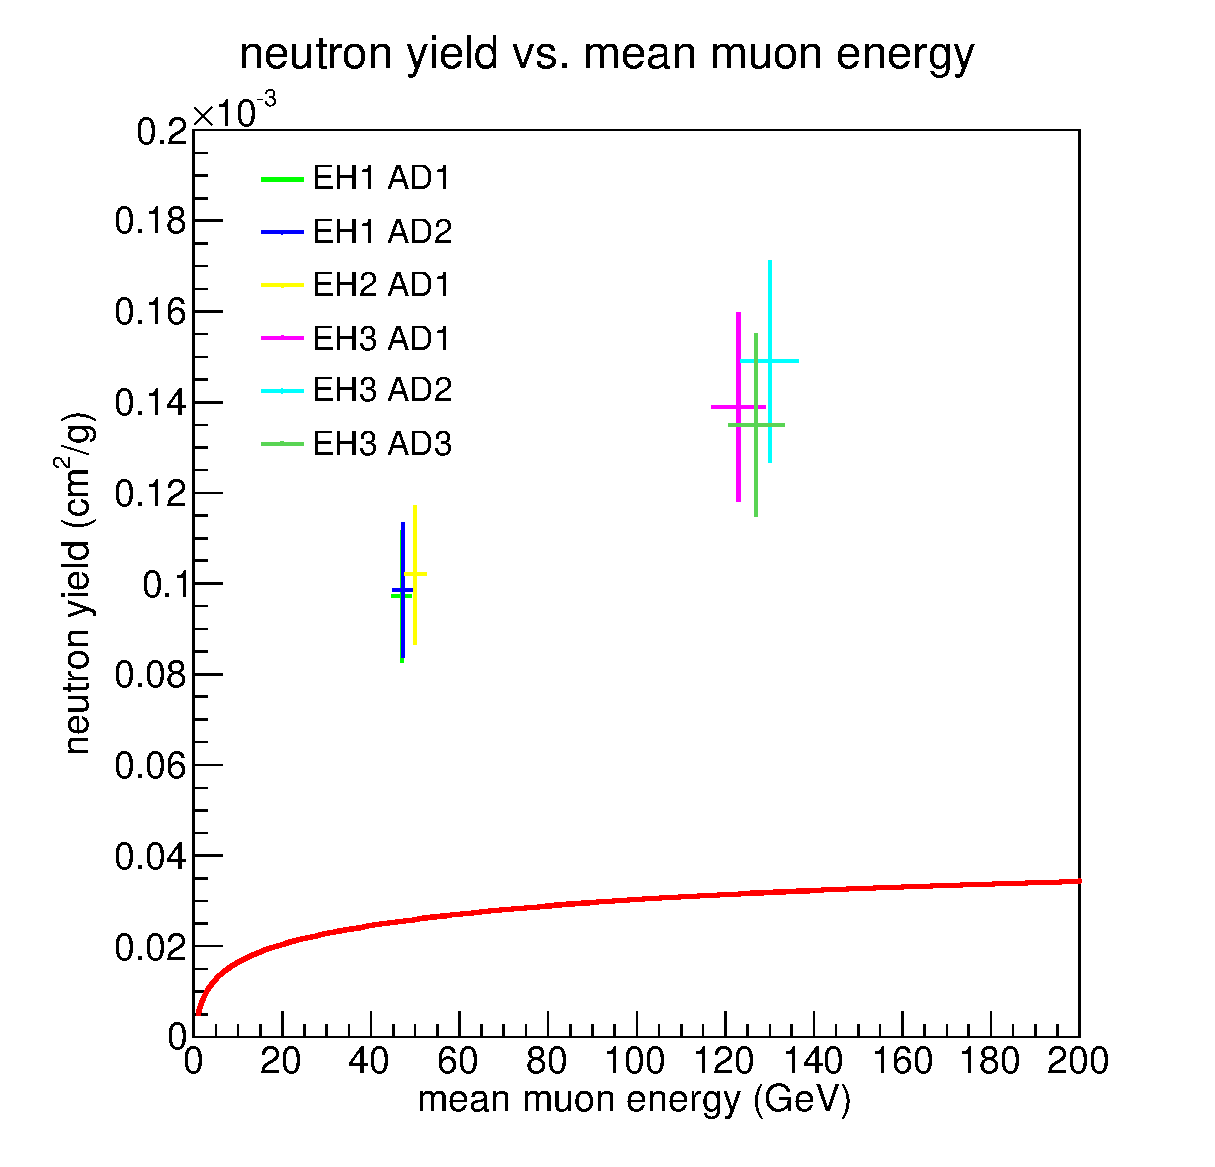
\includegraphics[width=.8\textwidth]{figures/chap7/yield_vs_energy_thesis.eps}
	\caption{Neutron yield as a function of the mean muon energy. The red curve is the calculated yield from the muon spallation process under the assumptions made in Chapter~\ref{chap:yield_theory}.}
	\label{fig:yield_vs_energy}
\end{figure}

Since muon trajectories are able to be reconstructed, the muon energy loss can be studied.
\begin{figure}
	\centering
	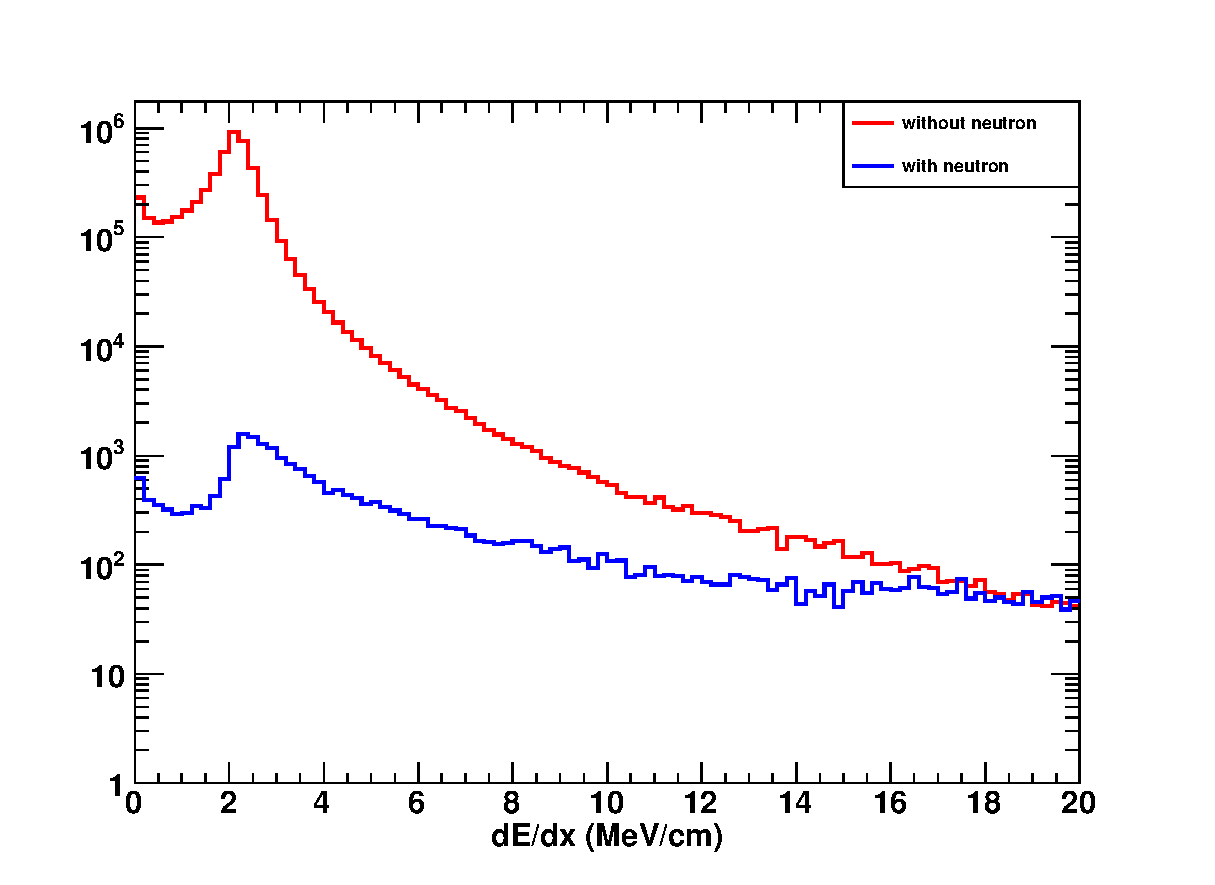
\includegraphics[width=.6\textwidth]{figures/chap7/dedx.eps}
	\caption{Muon energy loss for muons with and without induced neutrons.}
	\label{fig:dedx}
\end{figure}
Figure~\ref{fig:dedx} shows the muon energy loss in units of MeV/cm for muons with and without induced neutrons. The red histogram is the energy loss without associated neutrons and the blue one is the energy loss with associated neutrons. First we see both histograms peak at $\approx 2$ MeV/cm, corresponding to the minimum ionizing particles. However, the blue curve with-neutron histogram has a flatter tail, indicating extra energy deposition for muons with produced neutrons compared with those without produced neutrons.
  \chapter{Conclusion}

The Daya Bay Reactor Neutrino Experiment is a precision measurement of $\theta_{13}$ designed to measure $\sin^22\theta_{13}$ with sensitivity $<0.01$ at 90\% confidence level. In 2012 Daya Bay discovered that $\theta_{13}$ is nonzero with 5.2$\sigma$ and $\sin^22\theta_{13}=0.092\pm0.016(\text{stat.})\pm0.005(\text{syst.})$~\cite{dayabay2012_1}. The fast neutron background constitutes one of the five backgrounds in $\theta_{13}$ measurement. Therefore understanding the neutron yield induced by cosmic ray muons is important.

In this study we make a well-defined cylindrical fiducial volume of fixed radius around each muon track. Only neutrons captured in the fiducial volume is counted. We use the lateral distribution of the neutron captured position to correct for the inefficiency due to the neutrons leaking out of the fiducial volume.

The muon tracks are reconstructed by connecting the RPC and OWS reconstructed points. The RPC positions are reconstructed by the centroids of the fired $x$ and $y$ strips with a resolution of $\sim 7$ cm. The OWS positions are reconstructed by the charge-weighted mean of the positions of fired PMTs whose resolution is $\sim 60$ cm. The neutron captured positions are reconstructed by charge-weighted mean corrected by Monte Carlo simulation with a resolution of $\sim 20$ cm. The resolutions of the reconstruction algorithms are used for estimating errors in the neutron yield determination. Details in constructing the fiducial volumes can be found in Appendix~\ref{app:a}.

The neutron yield produced by muons in liquid scintillator was measured at Daya Bay to be about $10^{-4} cm^2/\mu/g$. These results are in agreement with previous measurements~\cite{Agafonova2013}. Figure~\ref{fig:neutron_yield_chap8} shows the results obtained in this study on top of the previous measurements.
\begin{figure}
	\centering
	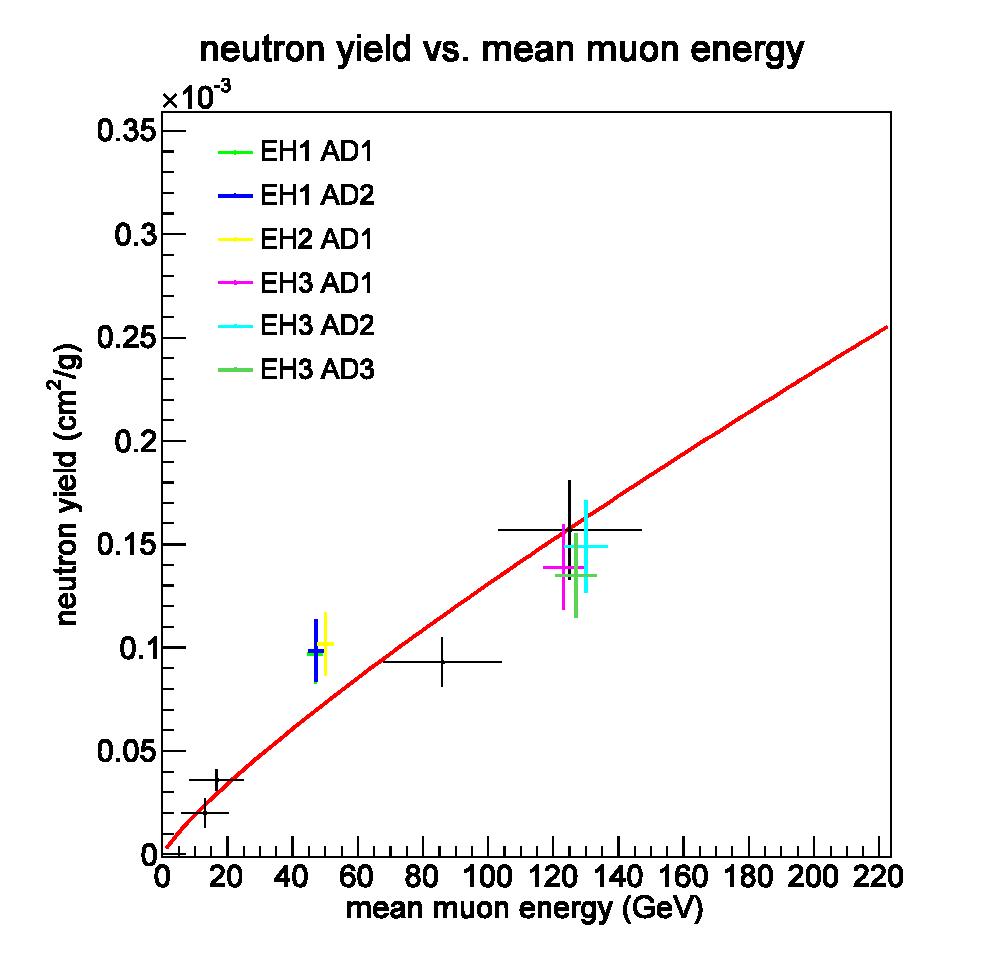
\includegraphics[width=0.7\textwidth]{figures/chap8/neutron_yield.eps}
	\caption[Neutron yield as a function of the mean muon energy. Colored points are results in this study. Black dots are from previous measurements. The red curve is the power law fit to the black dots.]{Neutron yield as a function of the mean muon energy. Colored points are results in this study. Black dots are from previous measurements~\cite{Agafonova2013}. The red curve is the power law fit to the black dots.}
	\label{fig:neutron_yield_chap8}
\end{figure}
We also found evidence for additional energy deposition in neutron events.


%\clearpage % start a new page for references
  %\input{EventRate.tex}

	\appendix
  \chapter{Geometric Problems Related to Muon Physics at Daya Bay}\label{app:a}
The Daya Bay neutrino experiment is equipped with excellent muon tracker detectors, thus more aspects of the muon physics can be studied by reconstructing muon tracks. Since in each collision the muon deflection is usually small, the muon track is usually approximated by a straight line. Besides, detectors usually are of regular shapes such as being spherical or cylindrical, they can by modeled by simple 3D algebraic equations. There are several interesting questions concerning to the relations between different geometric objects and in this appendix simple solutions to these pure analytic geometry problems are presented.

\section{Track Length in a Cylinder}
At Daya Bay the deposited energy of each muon is registered. Since the ionization energy loss is roughly proportional to the track length the muon traverses, track length is also a quantity of interest. Because the energy registered by the detector is mainly from the scintillation light when the muon passes the scintillator region, we are interested in the track length contained in the outer acrylic vessel where liquid scintillator resides. Besides, neutrons are detected mainly by the Gd capture and Gd is only present inside the inner acrylic vessel. When measuring the neutron production per unit length, the track length inside the IAV is also needed. Here we want to solve the problem that given a cylinder centered at the origin and a straight line passing through it, find the length of the line inside the cylinder.

\paragraph{Problem:}Given a cylinder with radius $r$ and height $2r$ and a straight line intersecting with the cylinder which passes a point $\vec{p}$ with a normalized direction vector $\hat{v}$, find the length of the line segment contained in the cylinder.

\paragraph{Solution:}
One way to solve this problem is to write down the equations for the the cylinder and the straight line in some convenient coordinate system and solve for the intersection points. However when implementing this method in computer codes, the idea is obscured by the lines of code to solve the simultaneous algebraic equations. Another more coordinate free and clearer to implement method is stated below.

First we deal with the intersection problem of the straight line with an infinitely long cylinder. After the intersection points are found, the top and bottom planes are restored, and the intersection points are adjusted if necessary. The axis of the cylinder is also a straight line and together with the track line form two skew lines. The closest distance $d$ between the skew lines can be used to identify whether the track line intersects the cylinder and is easily found. Suppose the points where the closest distance happens are $\vec{q}_c$ on the cylinder axis and $\vec{q}$ on the track line. $\vec{q}_c$ and $\vec{q}$ satisfy the equations
\begin{eqnarray}
	\vec{q}_c&=&\vec{p}_c+t_c\hat{v}_c \\
	\vec{q}&=&\vec{p}+t\hat{v}
\end{eqnarray}
where $\vec{p}_c$, $\hat{v}_c$ are the point and the direction vector of the cylinder axis and $t_c$ and $t$ are the parameters to be determined. Since the line formed by the two closest points is perpendicular to both of the skew lines, the vector $\vec{q}-\vec{q}_c$ is parallel to the cross product of the direction vectors of the skew lines,
\begin{equation}\label{closest_app_orig}
	\vec{q}-\vec{q}_c=\vec{p}-\vec{p}_c+t\hat{v}-t_c\hat{v}_c=k\hat{v}\times\hat{v}_c
\end{equation}
Let $\vec{p}_r=\vec{p}-\vec{p}_c$ and $\vec{n}=\hat{v}\times\hat{v}_c$, Equation~\ref{closest_app_orig} becomes
\begin{equation}\label{closest_app}
	\vec{p}_r+t\hat{v}-t_c\hat{v}_c=k\vec{n}
\end{equation}
Dot Equation~\ref{closest_app} with $\vec{n}$ on both sides and note that $\vec{n}\cdot \hat{v}=\vec{n}\cdot \hat{v}_c=0$, we have
\begin{equation}
	kn^2=\vec{p}_r\cdot \vec{n}
\end{equation}
Therefore the closest distance $d$ is given by
\begin{equation}
	d=\abs{\vec{q}-\vec{q}_c}=\abs{kn}=\frac{\abs{\vec{p}_r\cdot \vec{n}}}{n}=\frac{\abs{(\vec{p}-\vec{p}_c)\cdot (\hat{v}\times\hat{v}_c)}}{\abs{\hat{v}\times\hat{v}_c}}
\end{equation}
Note that if $d>r$ then the track line will never intersect the cylinder and there is no solution to this problem.

To find the parameters $t$ and $t_c$, first form the cross product of both sides of Equation~\ref{closest_app} with $\vec{n}$
\begin{equation}\label{par_eq}
	\vec{p}_r\times \vec{n}+t\hat{v}\times \vec{n}-t_c\hat{v}_c\times \vec{n}=0
\end{equation}
Now to get $t$, dot both sides of Equation~\ref{par_eq} with $\vec{v}_c$ and note that $\vec{v}_c\cdot (\vec{v}_c\times \vec{n})=0$ and $\vec{v}_c\cdot (\vec{v}\times \vec{n})=(\vec{v}_c\times \vec{v})\cdot \vec{n}=-n^2$. Then we get
\begin{equation}
	t=\vec{v}_c\cdot (\vec{p}_r\times \vec{n})/n^2
\end{equation}
Similarly we can dot Equation~\ref{par_eq} with $\vec{v}$ to obtain $t_c$.

Now that we have the shortest distance between the skew lines and the corresponding points, we are ready to solve for the intersection points. Figure~\ref{fig:cyl_line} shows a cylinder in blue and a straight line in red passing through it. $\overleftrightarrow{CD}$ is the cylinder axis and $\overleftrightarrow{Q_iQ_o}$ is the track line. Given the closest points $O$, $Q$, and angle $\angle QQ_iB=\angle QQ_oA=\theta$, we want to find $\ell=\overline{QQ_i}=\overline{QQ_o}$.
\begin{figure}
	\centering
	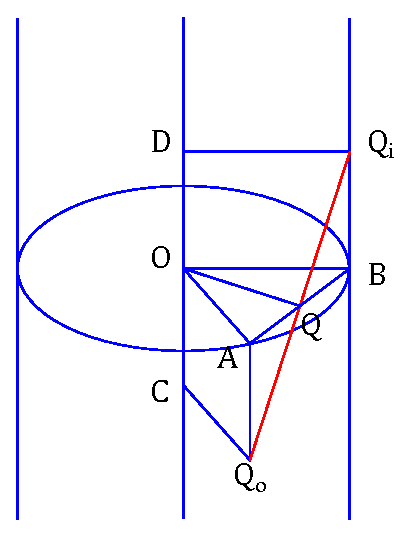
\includegraphics[width=.4\textwidth]{figures/appendixA/cylinder_line.eps}
	\caption{An illustration of a cylinder and a straight line passing through it. Given points $O$ and $Q$, we want to find $Q_i$ and $Q_o$.}
	\label{fig:cyl_line}
\end{figure}

$\ell$ can actually be found by simple arguments. First we start from $Q_i$ and draw a straight line on the cylinder surface parallel to the cylinder axis. This line will intersect with the circle centered at $O$. We call the point $B$. Similarly we can find point $A$ starting with point $Q_o$. Since $\overline{OA}=\overline{OB}=r$, the radius of the cylinder, $\triangle OAB$ is isoceles. By symmetry, $\triangle OQA$ is congruent to $\triangle OQB$, and therefore $\overline{OQ}$ is perpendicular to $\overline{AB}$. Meanwhile, $\triangle QBQ_i$ and $\triangle QAQ_o$ are also right triangles. From $\triangle OQB$ and $\triangle QBQ_i$ we have the relation
\begin{gather}
  \overline{QB}^2=\ell^2\sin^2\theta=\overline{OB}^2-\overline{OQ}^2 \\
  \Rightarrow \ell=\frac{\sqrt{r^2-d^2}}{\sin\theta}
\end{gather}
Once $\ell$ is known, $Q_i$ and $Q_o$ are also known.

The last step is to restore the top and bottom planes of the cylinder and rescale the solution points if necessary. In order to simply the notation, here we adopt the coordinate system with the origin at the cylinder center and the $z$ axis parallel to the cylinder axis. In this coordinate system the top cylinder plane has the equation $z=z_t$ and bottom plane has the equation $z=z_b$. Suppose in this coordinate system $Q_i$ has coordinate $Q_i(q_{ix},q_{iy},q_{iz})$. There are three conditions concerning to the ordering of $q_{iz}$, $z_t$ and $z_b$:
\begin{enumerate}
	\item $q_{iz}<z_b$. There is no solution to this problem.
	\item $z_b<q_{iz}<z_t$. $Q_i$ is the right answer and nothing has to be done.
	\item $z_t<q_{iz}$. $Q_i$ has to be moved along the track line until it touches the top plane. The new point is
	\begin{equation}
		\vec{q'}_i=\vec{q}-\frac{z_t-q_z}{q_{iz}-q_z}\hat{v}
	\end{equation}
	where $Q$ has the coordinate $Q(q_x,q_y,q_z)$ and $\hat{v}$ has a direction with $v_z<0$.
\end{enumerate}

We do a similar check on the point $Q_o$. If there is a solution, the track length is $\overline{Q_iQ_o}$.

Now we look at the problem of finding a cylindrical fiducial volume with an arbitrary axis inside a bigger cylinder so that it has the maximum length and is completely inscribed in the bigger cylinder.

\paragraph{Problem:} Given a cylinder with radius $R$ and height $2R$, a straight line with a point $p_0$ and a normalized direction $\hat{v}$, find a cylinder with the straight line as its axis and a fixed radius $r<R$ such that the cylinder has a maximum  length and is completely inside the given cylinder.

\paragraph{Solution:} We use the coordinate system centered at the center of the given cylinder with $z$ axis parallel to the cylinder axis. Again we start with two infinitely long cylinders, one with radius $R$ and the other with radius $r<R$. If they do intersect, the intersection is a curve. First we want to find, at least numerically, the coordinates of the points in the curve.
\begin{figure}
	\centering
	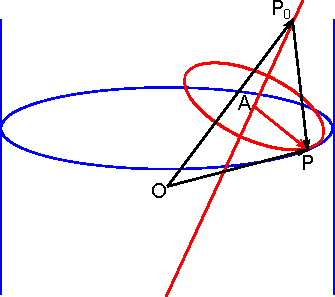
\includegraphics[width=.5\textwidth]{figures/appendixA/inscribe.pdf}
	\caption{A point $P$ belonging to the surface of the big and small cylinders simultaneously.}
	\label{fig:inscribe}
\end{figure}
Figure~\ref{fig:inscribe} shows a point $P$ belonging to the given and the fiducial cylinders simultaneously. Since $P$ is on the fiducial cylinder, from Pythagorean theorem we have
\begin{equation}\label{eq:pytha}
	\overline{AP_0}^2+\overline{AP}^2=\overline{PP_0}^2
\end{equation}
Now $\overline{AP_0}=r$, $\overline{AP}=|(\vec{p}-\vec{p}_0)\cdot \hat{v}|$, $\overline{PP_0}=|\vec{p}-\vec{p}_0|$. Because $P$ also belongs to the given cylinder, it has coordinate $P(R\cos\phi,R\sin\phi,z)$. Suppose $\vec{p}-\vec{p}_0=(X,Y,Z)$ and $\hat{v}=(v_x,v_y,v_z)$, by substituting the coordinates and numbers into Equation~\ref{eq:pytha} we obtain
\begin{equation}
	(1-v_z^2)Z-2v_z(v_xX+v_yY)Z+[X^2+Y^2-(v_xX+v_yY)^2-r^2]=0
\end{equation}
where
\begin{eqnarray}
	X &=& R\cos\phi-p_{0x} \\
	Y &=& R\sin\phi-p_{0y} \\
	Z &=& z-p_{0z}
\end{eqnarray}
For each value of $\phi$ there is a corresponding quadratic equation. Practically we can scan for $\phi$ with some small step, solve the equation for $z$, and find the coordinates of the points in the common curve. Usually there are $\phi$ values with two real roots and $\phi$ values without any real root. This is due to the topology of the intersection curve. We plot the $z$ versus $\phi$ plot. If there is solution to this problem, there are two closed curve in this plot. If there are less then two curves, there is no solution. Figure~\ref{fig:no_solution_cylinders} and Figure~\ref{fig:with_solution_cylinders} show examples without and with solution. From the figures we clearly see that the problem has a solution only if there are two closed curves.
\begin{figure}
	\centering
  \subfloat[$z$ vs. $\phi$]{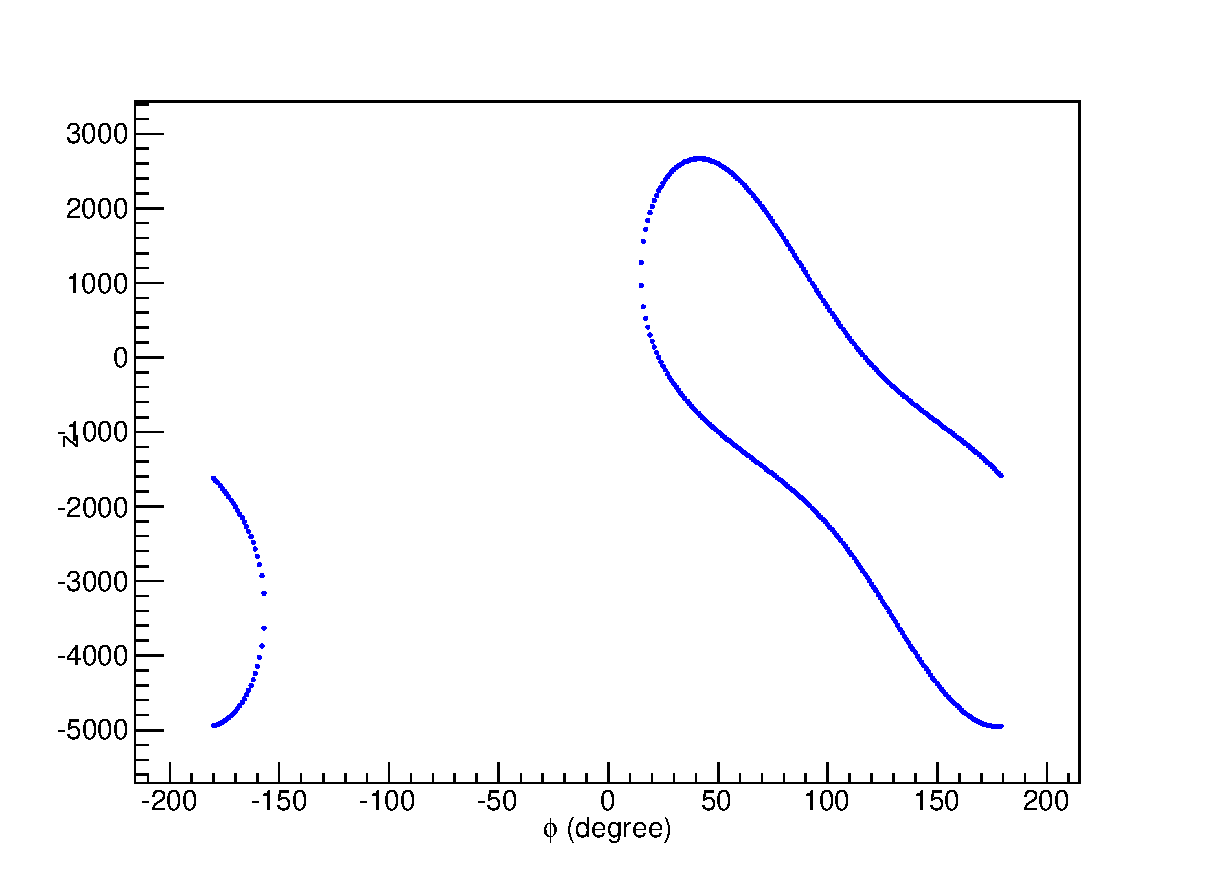
\includegraphics[height=.25\textheight]{figures/appendixA/curve1.eps}}
  \qquad
	\subfloat[3D Model]{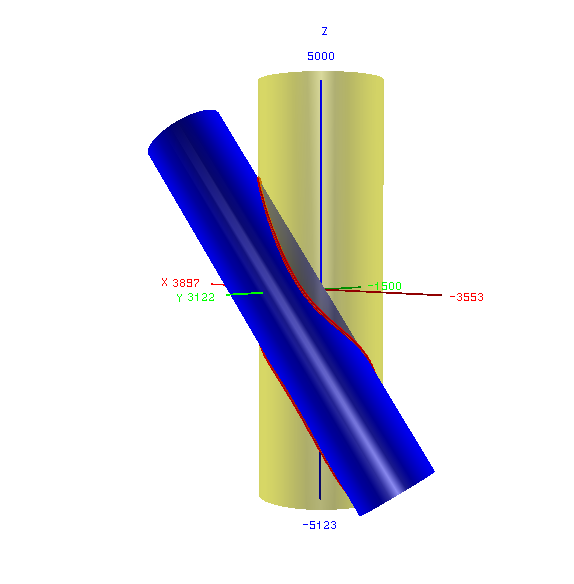
\includegraphics[height=.25\textheight]{figures/appendixA/cyl1.png}}
	\caption{The $z-\phi$ plot and the 3D model of an example without solution.}
	\label{fig:no_solution_cylinders}
\end{figure}
\begin{figure}
	\centering
  \subfloat[$z$ vs. $\phi$]{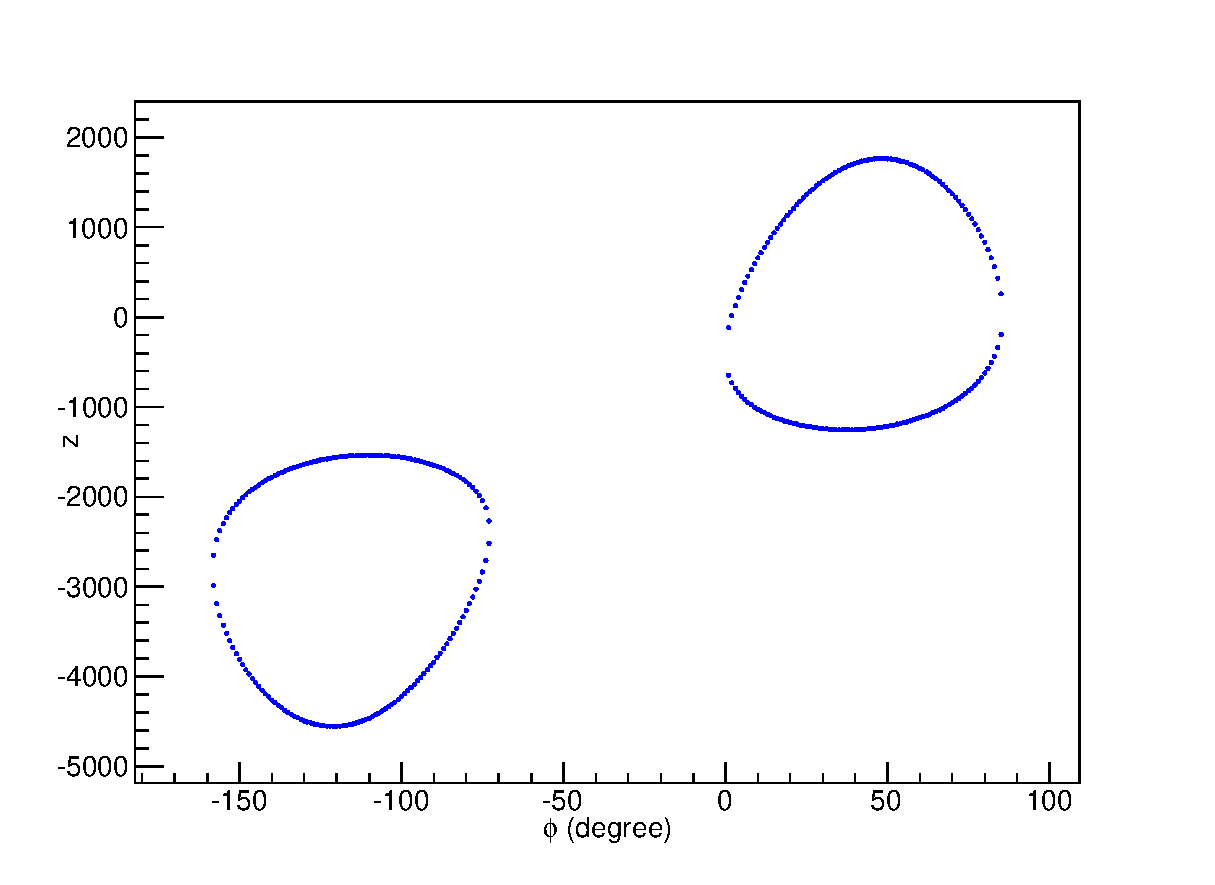
\includegraphics[height=.25\textheight]{figures/appendixA/curve2.eps}}
  \qquad
	\subfloat[3D Model]{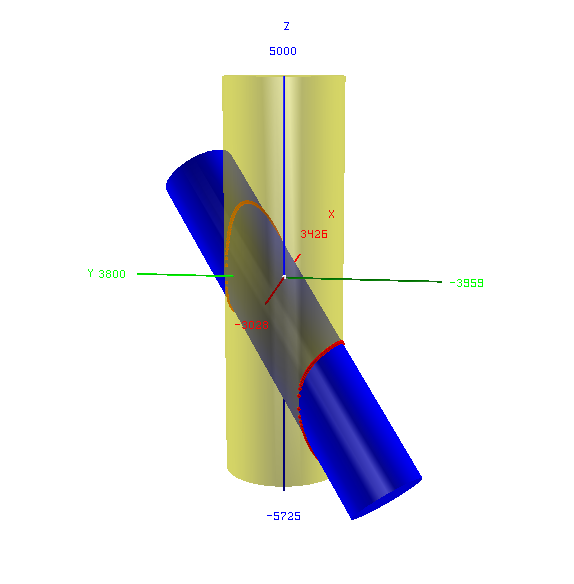
\includegraphics[height=.25\textheight]{figures/appendixA/cyl2.png}}
	\caption{The $z-\phi$ plot and the 3D model of an example with solution.}
	\label{fig:with_solution_cylinders}
\end{figure}
Here we also introduce a convenient track coordinate, with origin at the point of the track line $p_0$ and a $t$ axis along the track's direction vector $\hat{v}$. For each point in each closed curve we can calculate the $t$-value by projection,
\begin{equation}
	t=\left(\vec{p}-\vec{p}_0\right)\cdot \hat{v}
\end{equation}
Now we look for the four numbers,
\begin{eqnarray}
	t^{(i)}_M&=&\sup\left\{ t^{(i)}|\vec{p}^{(i)}\in C^{(i)}\right\} \\
	t^{(i)}_m&=&\inf\left\{ t^{(i)}|\vec{p}^{(i)}\in C^{(i)}\right\}
\end{eqnarray}
where $i=1,2$ for the two closed curves $C^{(i)}$, sort the four numbers, take the middle two numbers and call the larger one $t_{bot}$ and the smaller one $t_{top}$. Then we arrive at two candidate planes. Each one has $\hat{v}$ as its normal vector and passes $\vec{p}_{bot}=\vec{p}_0+t_{bot}\hat{v}$ and $\vec{p}_{top}=\vec{p}_0+t_{top}\hat{v}$, respectively.

Now we restore the top and bottom planes of the detector cylinder. If the top circle of the track cylinder protrudes the top plane of the detector cylinder, slide it along the track until it just touches the top plane of the detector cylinder. The same applies to the bottom circle of the track cylinder.
  
  \bibliographystyle{ieeetr}%Choose a bibliograhpic style
  \bibliography{mainmatter/references}
\end{document}